\documentclass[
	% -- opções da classe memoir --
	12pt,				% tamanho da fonte
	openright,			% capítulos começam em pág ímpar (insere página vazia caso preciso)
	oneside,			% para impressão em recto e verso. Oposto a oneside /twoside
	a4paper,			% tamanho do papel. 
	% -- opções da classe abntex2 --
	%chapter=TITLE,		% títulos de capítulos convertidos em letras maiúsculas
	%section=TITLE,		% títulos de seções convertidos em letras maiúsculas
	%subsection=TITLE,	% títulos de subseções convertidos em letras maiúsculas
	%subsubsection=TITLE,% títulos de subsubseções convertidos em letras maiúsculas
	% -- opções do pacote babel --
	english,			% idioma adicional para hifenização
	%french,				% idioma adicional para hifenização
	%spanish,			% idioma adicional para hifenização
	brazil				% o último idioma é o principal do documento
	]{abntex2}

% ---
% Pacotes básicos 
% ---
\usepackage{times}			% Usa a fonte Latin Modern			
\usepackage[T1]{fontenc}		% Selecao de codigos de fonte.
\usepackage[utf8]{inputenc}		% Codificacao do documento (conversão automática dos acentos)
\usepackage{lastpage}			% Usado pela Ficha catalográfica
\usepackage{indentfirst}		% Indenta o primeiro parágrafo de cada seção.
\usepackage{color}				% Controle das cores
\definecolor{mygreen}{RGB}{28,172,0} % color values Red, Green, Blue
\definecolor{mylilas}{RGB}{170,55,241}
\usepackage{graphicx}			% Inclusão de gráficos
\usepackage{microtype} 			% para melhorias de justificação
\usepackage{mathtools}
\usepackage{subcaption}
\usepackage{algpseudocode,algorithm}
\usepackage{tikz}
\usepackage{listings}
\usepackage[final]{pdfpages}
\usepackage{verbatim}
\usepackage{amssymb}
\usetikzlibrary{shapes,arrows}
\usepackage{rotating}
\usepackage{colortbl}

\usetikzlibrary{trees}

\newcommand\grbox[2]{%
\begin{tabular}{!{\kern-\tabcolsep}p{4.27cm}c@{}}%
#1&{#2}\end{tabular}}


\captionsetup[subfigure]{justification=centering}

%Pseudo Código
% Declaracoes em Português
\algrenewcommand\algorithmicend{\textbf{fim}}
\algrenewcommand\algorithmicdo{\textbf{faça}}
\algrenewcommand\algorithmicwhile{\textbf{enquanto}}
\algrenewcommand\algorithmicfor{\textbf{para}}
\algrenewcommand\algorithmicif{\textbf{se}}
\algrenewcommand\algorithmicthen{\textbf{então}}
\algrenewcommand\algorithmicelse{\textbf{senão}}
\algrenewcommand\algorithmicreturn{\textbf{retorne}}
\algrenewcommand\algorithmicfunction{\textbf{função}}
\algrenewcommand\algorithmicrepeat{\textbf{repita}}
\algrenewcommand\algorithmicuntil{\textbf{até}}

% Rearranja os finais de cada estrutura
\algrenewtext{EndWhile}{\algorithmicend\ \algorithmicwhile}
\algrenewtext{EndFor}{\algorithmicend\ \algorithmicfor}
\algrenewtext{EndIf}{\algorithmicend\ \algorithmicif}
\algrenewtext{EndFunction}{\algorithmicend\ \algorithmicfunction}

\algnewcommand{\LeftComment}[1]{\State \(\triangleright\) #1}
\algnewcommand{\LeftTextComment}[1]{\State \(\) #1}


\makeatletter
\renewcommand{\ALG@name}{Algoritmo}
\makeatother
\renewcommand{\listalgorithmname}{Lista de Algoritmos}

%Para usar acentos no lstlisting
\lstset{
  literate={á}{{\'a}}1
           {ó}{{\'o}}1
           {é}{{\'e}}1
}

\lstdefinelanguage{JavaScript}{
  keywords={typeof, new, true, false, catch, function, return, null, catch, switch, var, if, in, while, do, else, case, break},
  keywordstyle=\color{blue}\bfseries,
  ndkeywords={class, export, boolean, throw, implements, import, this},
  ndkeywordstyle=\color{darkgray}\bfseries,
  identifierstyle=\color{black},
  sensitive=false,
  comment=[l]{//},
  morecomment=[s]{/*}{*/},
  commentstyle=\color{green}\ttfamily,
  stringstyle=\color{red}\ttfamily,
  morestring=[b]',
  morestring=[b]"
}

\lstset{
   language=JavaScript,
   backgroundcolor=\color{white},
   extendedchars=true,
   basicstyle=\footnotesize\ttfamily,
   showstringspaces=false,
   showspaces=false,
   numbers=left,
   numberstyle=\footnotesize,
   numbersep=9pt,
   tabsize=2,
   breaklines=true,
   showtabs=false,
   captionpos=b
}

% ---
		
\usetikzlibrary{fit}
\tikzset{%
  highlight/.style={rectangle,rounded corners,fill=red!15,draw,fill opacity=0.5,thick,inner sep=0pt}
}
\newcommand{\tikzmark}[2]{\tikz[overlay,remember picture,baseline=(#1.base)] \node (#1) {#2};}
%
\newcommand{\Highlight}[1][submatrix]{%
    \tikz[overlay,remember picture]{
    \node[highlight,fit=(left.north west) (right.south east)] (#1) {};}
}
\captionsetup[subfigure]{subrefformat=simple,labelformat=simple}
\renewcommand\thesubfigure{(\alph{subfigure})}

\renewcommand{\lstlistingname}{Código}

% sintax highlight for MatLab
\lstset{language=Matlab,%
    %basicstyle=\color{red},
    morekeywords={matlab2tikz},
    keywordstyle=\color{blue},%
    morekeywords=[2]{1}, keywordstyle=[2]{\color{black}},
    identifierstyle=\color{black},%
    stringstyle=\color{mylilas},
    commentstyle=\color{mygreen},%
    showstringspaces=false,%without this there will be a symbol in the places where there is a space
    numbers=left,%
    numbersep=9pt, % this defines how far the numbers are from the text
    emph=[1]{for,end,break},emphstyle=[1]\color{red}, %some words to emphasise
    basicstyle=\small\sffamily,
	numberstyle=\tiny,
	frame=tb,
	columns=fullflexible,
	showstringspaces=false 
}

% ---

% ---
% Pacotes de citações
% ---
\usepackage[alf]{abntex2cite}	% Citações padrão ABNT

% --- 
% CONFIGURAÇÕES DE PACOTES
% --- 

% ---
% Configurações do pacote backref
% Usado sem a opção hyperpageref de backref
% ---
% --
% Informações de dados para CAPA e FOLHA DE ROSTO
% ---
\titulo{Refinamento de Buscas por Imagens Digitais Utilizando Nuvens Dinâmicas}
\autor{Efraim Naassom Helem Dantas Rodrigues}
\local{Mossoró-RN}
\data{2017}
\orientador{Prof. Dr. Leandro Carlos de Souza}
\instituicao{%
  Universidade Federal Rural do Semi-Árido -- UFERSA
  \par
  Centro de Ciências Exatas e Naturais -- CCEN
  \par
  Curso de Ciência da Computação}
\tipotrabalho{Monografia}
% O preambulo deve conter o tipo do trabalho, o objetivo, 
% o nome da instituição e a área de concentração 
\preambulo{Trabalho de Conclusão de Curso apresentado ao Curso de Ciência da Computação da Universidade Federal Rural do Semi-Árido como requisito parcial para a obtenção do grau de bacharel em Ciência da Computação.}
% ---


% ---
% Configurações de aparência do PDF final

% alterando o aspecto da cor azul
%\definecolor{blue}{RGB}{0,0,0}

% informações do PDF
\makeatletter
\hypersetup{
     	%pagebackref=true,
		pdftitle={\@title}, 
		pdfauthor={\@author},
    	pdfsubject={\imprimirpreambulo},
	    pdfcreator={LaTeX with abnTeX2},
		pdfkeywords={abnt}{latex}{abntex}{abntex2}{trabalho acadêmico}, 
		colorlinks=true,       		% false: boxed links; true: colored links
    	linkcolor=black,          	% color of internal links
    	citecolor=black,        		% color of links to bibliography
    	filecolor=black,      		% color of file links
		urlcolor=blue,
		bookmarksdepth=4
}
\makeatother
% --- 

% --- 
% Espaçamentos entre linhas e parágrafos 
% --- 

% O tamanho do parágrafo é dado por:
\setlength{\parindent}{1.3cm}

% Controle do espaçamento entre um parágrafo e outro:
\setlength{\parskip}{0.2cm}  % tente também \onelineskip

% ---
% compila o indice
% ---
\makeindex
% ---

% ----
% Início do documento
% ----
\begin{document}

% Seleciona o idioma do documento (conforme pacotes do babel)
%\selectlanguage{english}
\selectlanguage{brazil}

% Retira espaço extra obsoleto entre as frases.
\frenchspacing 

\renewcommand{\imprimircapa}{%
\begin{capa}%
\center
\begin{figure}
\centering
\includegraphics[width=150px]{figures/PNG-logo-Ufersa.png}
\end{figure}
\vspace*{-1.4cm}
\ABNTEXchapterfont UNIVERSIDADE FEDERAL RURAL DO SEMI-ÁRIDO - UFERSA \\
\ABNTEXchapterfont PRÓ-REITORIA DE GRADUAÇÃO \\
\ABNTEXchapterfont CENTRO DE CIÊNCIAS EXATAS E NATURAIS \\
\ABNTEXchapterfont CURSO DE CIÊNCIA DA COMPUTAÇÃO

\vspace*{3cm}

{\ABNTEXchapterfont\large\imprimirautor}

\vfill
\begin{center}
\ABNTEXchapterfont\bfseries\LARGE\imprimirtitulo
\end{center}
\vfill

\large\imprimirlocal

\large\imprimirdata

\vspace*{1cm}
\end{capa}
}

% ----------------------------------------------------------
% ELEMENTOS PRÉ-TEXTUAIS
% ----------------------------------------------------------
% \pretextual

% ---
% Capa
% ---
\imprimircapa
% Capa sem o uso de \capa
% ---

% ---
% Folha de rosto
% (o * indica que haverá a ficha bibliográfica)
% ---

\makeatletter
\renewcommand{\folhaderostocontent}{
\begin{center}

    %\vspace*{1cm}
    {\ABNTEXchapterfont\large\imprimirautor}
	
    \vspace*{\fill}\vspace*{\fill}
    \begin{center}
      \ABNTEXchapterfont\bfseries\Large\imprimirtitulo
    \end{center}
    \vspace*{\fill}
	
    \abntex@ifnotempty{\imprimirpreambulo}{%
      \hspace{.45\textwidth}
      \begin{minipage}{.5\textwidth}
      	\SingleSpacing
         \imprimirpreambulo
         \\ 
         \SingleSpacing
         \imprimirorientadorRotulo~\imprimirorientador\par
       \end{minipage}%
       \vspace*{\fill}
    }%

    \vspace*{\fill}

    {\large\imprimirlocal}
    \par
    {\large\imprimirdata}
    \vspace*{1cm}

  \end{center}
}
\makeatother

\imprimirfolhaderosto*
% ---

% ---
% Inserir a ficha bibliografica
% ---

% Isto é um exemplo de Ficha Catalográfica, ou ``Dados internacionais de
% catalogação-na-publicação''. Você pode utilizar este modelo como referência. 
% Porém, provavelmente a biblioteca da sua universidade lhe fornecerá um PDF
% com a ficha catalográfica definitiva após a defesa do trabalho. Quando estiver
% com o documento, salve-o como PDF no diretório do seu projeto e substitua todo
% o conteúdo de implementação deste arquivo pelo comando abaixo:
%
\begin{fichacatalografica}
     \includepdf{fichacatalografica.pdf}
\end{fichacatalografica}

% ---
% Inserir folha de aprovação
% ---

% Isto é um exemplo de Folha de aprovação, elemento obrigatório da NBR
% 14724/2011 (seção 4.2.1.3). Você pode utilizar este modelo até a aprovação
% do trabalho. Após isso, substitua todo o conteúdo deste arquivo por uma
% imagem da página assinada pela banca com o comando abaixo:
%
\includepdf{deferimentoFinal.pdf}
%

% ---
% Agradecimentos
% ---
%\begin{agradecimentos}


%\end{agradecimentos}
% ---

% ---
% Epígrafe
% ---
\begin{epigrafe}
    \vspace*{\fill}
	\begin{flushright}
		\textit{Soli Deo Gloria \\
		}
	\end{flushright}
\end{epigrafe}
% ---

% ---
% RESUMOS
% ---

% resumo em português
\setlength{\absparsep}{18pt} % ajusta o espaçamento dos parágrafos do resumo
\begin{resumo}
Com a popularização dos dispositivos de aquisição de imagens e da \emph{INTERNET}, milhares de imagens estão disponíveis para busca. É possível recuperar e acessar imagens públicas através de motores de busca, como o do \emph{Google}, por exemplo.  Em virtude do grande volume de imagens disponíveis em diversos acervos, torna-se necessário o desenvolvimento de métodos que possam selecionar e refinar os resultados desejados. Neste contexto, algoritmos de classificação propõem a organização de elementos de um conjunto utilizando agrupamento e classificação. Assim, é possível utilizar estes algoritmos para organizar resultados de buscas de imagens de tal modo que elas fiquem agrupadas por características afins. Desta forma, este trabalho propõe a criação de um sistema para refinar e organizar conjuntos de imagens resultantes de uma busca na \emph{INTERNET}. Este refinamento consiste em agrupar os resultados semelhantes entre si em pastas, auxiliando o usuário em sua busca. Os métodos aqui estudados envolvem o agrupamento de imagens por meio de nuvens dinâmicas e de descritores que representam as informações contidas nas mesmas.

 \textbf{Palavras-chave}: Nuvens dinâmicas. recuperação de imagens. agrupamento de imagens. internet.
\end{resumo}

% resumo em inglês
\begin{resumo}[Abstract]
 \begin{otherlanguage*}{english}
 Due the growing popularity of image acquisition devices and INTERNET, millions of images are available. It is possible to retrieve and access public images through search engines, such as Google's for instance. Because of the huge amount of available images in many repositories, the development of methods that can select and filter desired results is crucial. In this context classification algorithms aim to sort elements of a set using clustering and categorization. Thus it is possible to apply these algorithms to sort results from a search for images in such a manner that they are grouped according to related aspects. Hence, this work aim to create a system to filter and arrange sets of images retrieved from a search on the INTERNET. This filter intent to group similar elements in folders to aid users throughout search. The approaches in this work involve the categorization of images through dynamic clustering and descriptors that represent the information within the images.
   
   \textbf{Keywords}: Dynamic clustering. image retrieval. image clustering. content based image retrieval. internet.
 \end{otherlanguage*}
\end{resumo}

% ---

% ---
% inserir lista de ilustrações
% ---
\pdfbookmark[0]{\listfigurename}{lof}
\listoffigures*
\cleardoublepage
% ---

% ---
% inserir lista de tabelas
% ---
%\pdfbookmark[0]{\listtablename}{lot}
\listoftables*
%\cleardoublepage
% ---

% ---
% inserir lista de algoritmos
% ---
\pdfbookmark[0]{\listtablename}{lot}
\listofalgorithms
\cleardoublepage

% ---
% inserir lista de abreviaturas e siglas
% ---
\begin{siglas}
	\item[CBIR] Content Based Image Retrieval
	\item[CSS] Cascading Style Sheets
	\item[HTML] Hypertext Markup Language
	\item[HTTP] Hypertext Transfer Protocol
	\item[PDI] Processamento Digital de Imagens
	\item[SDK] Software Development Kit
	\item[TBIR] Text Based Image Retrieval
	\item[URI] Uniform Resource Identifiers
	\item[URL] Uniform Resource Locator  
\end{siglas}
% ---


% ---
% inserir o sumario
% ---
\pdfbookmark[0]{\contentsname}{toc}
\tableofcontents*
\cleardoublepage
% ---



% ----------------------------------------------------------
% ELEMENTOS TEXTUAIS
% ----------------------------------------------------------
\textual

                                                                                                                                                                                                                                      
\chapter[Introdução]{Introdução}
% ----------------------------------------------------------

Os avanços econômicos e tecnológicos das sociedades  facilitaram o acesso de grande parte da população a dispositivos tecnológicos com diversas funcionalidades, como permitir a aquisição e publicação de mídias na \emph{INTERNET}. Com uma quantidade massiva de indivíduos em posse destes dispositivos, uma grande quantidade de imagens digitais é gerada e publicada a todo instante na \emph{INTERNET}.

Em função da grande quantidade de mídias disponíveis, a necessidade de organização e sistematização da busca por informações tem sido tratada por grupos e estudiosos de todo o mundo. Diversos serviços de busca, como, por exemplo,  \emph{Google, Microsoft, Yahoo!} e \emph{Ask} foram desenvolvidos com o objetivo de resolver este tipo de problema. Entretanto, no contexto de imagens digitais, a maioria destes serviços suportam buscas relacionadas a termos descritivos das imagens e, em geral, não utilizam  características semânticas inerentes às mesmas.

O desenvolvimento de soluções para este tipo de problema se iniciou com base nas técnicas tradicionais de recuperação de imagens, como por exemplo relacionar uma classe de documentos à quantidade de vezes que uma palavra específica é encontrada. Entretanto algumas outras alternativas de métricas têm sido arquitetadas, como criar descritores estatísticos do conteúdo da imagem ou ainda combinar técnicas \cite{fundamentalsofmultimedia}.

Muitos mecanismos de recuperação de mídias digitais têm proposto soluções que consideram a semântica das mídias. Este tipo de recuperação é conhecido como recuperação de imagens baseada no conteúdo (CBIR) \cite{eakins}. As técnicas CBIR são relativamente novas, mas amplamente usadas para recuperação de imagens em bases de dados de larga escala \cite{jain2011survey}.

O principal objetivo das técnicas de resgate de imagens é auxiliar o usuário em recuperar imagens de maneira eficiente. Entretanto esta tarefa requer que o sistema entenda o real propósito de um usuário em uma busca. Por isso que as recuperações de imagens baseadas em texto (TBIR) e CBIR por si podem ser insatisfatórias. O fato é que a tarefa de entender o objetivo de um usuário em uma busca através de termos ou de uma imagem como parâmetros separados é desafiadora \cite{hartvedt2010using}. 

Este trabalho propõe uma ferramenta a ser usada  no navegador \emph{Mozilla Firefox} que pode auxiliar o usuário na tarefa de busca por imagens. A ferramenta proposta é uma extensão que é ativada quando o navegador carrega uma página de resultados de busca por imagem do \emph{Google}. A extensão não interfere na navegação por outras páginas, mas ao detectar a página de interesse, a aplicação carrega as imagens que estão sendo exibidas no \emph{browser} e as separa em grupos definidos por usuário de acordo com as semelhanças encontradas nos conteúdos das imagens.

\section{Problema}
Algoritmos para filtragem e organização de mídias associadas a textos são conhecidos e aplicados a serviços de busca. No contexto de busca de imagens por palavra-chave, as ferramentas tomam como parâmetro os termos associados à imagem desconsiderando o conteúdo da imagem. O problema é que estes filtros ou organização proposta por estas ferramentas podem não corresponder ao nível de semelhança esperado pelo usuário.

Os serviços de buscas de imagens \emph{on-line} não incluem, em seus algoritmos de filtragem de conteúdo, mecanismos de ordenação que fazem referências ao conteúdo das imagens. Desta forma as requisições retornam um grande número de imagens que não são organizadas levando em conta seus conteúdos. Assim, cabe ao usuário final a tarefa de filtrar visualmente o conteúdo das imagens a fim de se identificar quais delas correspondem ao resultado esperado.

\section{Objetivos}

\begin{comment}
\textbf{objetivos está muito seco, coloque mais um parágrafo indicando os objetivos específicos}
\end{comment}

O objetivo deste trabalho é a implementação de um algoritmo capaz de
classificar e organizar conjuntos de imagens resultantes do motor de busca do \emph{Google} a partir de semelhanças que as imagens apresentem em seus conteúdos. Para isto, pretende-se aplicar o método de nuvens dinâmicas, método de agrupamento indicado para dados complexos, nos autovetores dominantes e histogramas das imagens.

Para alcançar os objetivos gerais, este trabalho tem como objetivos específicos:

\begin{itemize}

\item Ter acesso a imagens de uma página de resultados do serviço de busca do \emph{Google};

\item Realizar a análise do conteúdo de imagens de uma página \emph{Web} e gerar descritores;

\item Empregar o algoritmo de agrupamento por nuvens dinâmicas;

\item Manipular a página \emph{Web} para exibir as imagens organizadas em grupos na própria página.

\end{itemize}

\section{Justificativa}
\begin{comment}
\textbf{Justificativa está muito seca, coloque mais coisas: buscas em bancos de imagens, aplicações médicas, busca de padrões para fenômenos climáticos através de fotos de satélite, etc...}
\end{comment}

Áreas como medicina, meteorologia e astronomia baseiam suas atividades em buscas feitas em volumosas bases de imagens que tendem a continuar crescendo. A busca por padrões e extração de conhecimento de base de dados tem se mostrado uma atividade vantajosa, não só para a ciência mas também para a economia \cite{berry1997data}.

Álbuns digitais (e.g., \emph{Flickr, Photobucket, Picasa}) e acervos de imagens de propósito geral são apontados como responsáveis para a tendência no aumento de publicação de imagens na \emph{INTERNET} \cite{hartvedt2010using}. Entretanto, estes serviços não dispõem de mecanismos de organização que levam em conta o conteúdo das imagens. Então, busca-se aperfeiçoar a experiência de usuários no uso de ferramentas de resgate de imagens.

\section{Organização}
Além deste capítulo introdutório, este documento é constituído de mais quatro capítulos.\\

\noindent
\textbf{Capítulo 2 - Referencial Teórico}\\
Este capítulo introduz os conceitos utilizados no desenvolvimento da aplicação proposta. A definição de imagem é apresentada, bem como a representação digital e os conceitos envolvidos no processo de sua aquisição. Além disso, são apresentados os conceitos de descritores e do algoritmo de agrupamento por nuvens dinâmicas. Também são expostos os conceitos essenciais implicados no funcionamento da \emph{INTERNET}.
\\

\noindent
\textbf{Capítulo 3 - Extensão para o \emph{Mozilla Firefox}}\\
O capítulo 3 descreve a metodologia utilizada para a solução do problema. As etapas de execução da aplicação são apresentadas.
\\

\noindent
\textbf{Capítulo 4 - Resultados}\\
O capítulo 4 apresenta uma discussão acerca dos resultados obtidos. 
\\

\noindent
\textbf{Capítulo 5 - Conclusão e Trabalhos Futuros}\\
Este capítulo expõe as percepções da solução proposta e direcionamentos que podem aprimorar a qualidade dos resultados e eficiência da aplicação.
\\

% ---
% Capitulo de revisão de literatura
% ---
\chapter{Referencial Teórico}

Uma imagem pode ser definida por uma função bidimensional $f(x,y)$ onde $x$ e $y$ são um par de coordenadas espaciais e $f$ em qualquer par de coordenadas $(x,y)$ representa a intensidade da imagem naquele ponto. Quando $x,y$ e os valores das intensidades de $f$ são todos finitos e em quantidades discretas, pode-se dizer que a imagem é uma imagem digital. Os  elementos  constituintes das imagens são denominados \emph{pels} ou \emph{pixels} \cite{Gonzalez:2006:DIP:1076432}. A quantidade de \emph{pixels} nas dimensões de altura e largura indicam a resolução de uma imagem. A Figura \ref{andressa}, mostra um exemplo de imagem monocromática digital cuja resolução é de 390x390, é representada matricialmente na Figura \ref{matriz-andressa}. 


\begin{figure}[htb]
\begin{center}
  \caption{(a) Exemplo de imagem digital (b) Representação matricial da imagem.}
  \begin{subfigure}[b]{0.6\textwidth}
  \centering
      \includegraphics[scale=0.6]{images/bw.png}
    \caption{}
    \label{andressa}
  \end{subfigure}
 %
  \begin{subfigure}[b]{0.6\textwidth}
  \centering
    \begin{center}
	%
	\sbox0{$\vcenter{\hbox{$\begin{bmatrix}
	0 & 0 & 0 & ...  & 0 & 0 \\ 
	0 & 0 & 0 &...  & 0 & 0\\ 
	\vdots & \vdots & \vdots & \vdots &  \vdots & \vdots \\ 
	0 & ... & 127 & ... & 0 & 0\\
	\vdots & \vdots & \vdots & \vdots &  \vdots & \vdots \\ 
	0 & 0 & 0 & ...  & 0 & 0
	\end{bmatrix}$}}$}%
	%
	$f(x,y)$ $=
	  \underbrace{\vrule width0pt depth \dimexpr\dp0 + .3ex\relax\copy0}_{w = 390}%
	  \left.\kern-\nulldelimiterspace
	    \vphantom{\copy0}
	  \right\rbrace \scriptstyle{h = 390}
	$
	\end{center}
    \caption{}
    \label{matriz-andressa}
  \end{subfigure}
  
  \legend{\textbf{Fonte:} \citeonline{Gonzalez:2006:DIP:1076432}.}
\end{center}

\end{figure}

O processamento digital de imagens (PDI) refere-se à utilização de métodos que manipulam imagens digitais e que geram como resultado outras imagens digitais. Apesar de a visão humana ser limitada ao espectro eletromagnético, dispositivos digitais podem operar em quase todo o espectro eletromagnético, realizando assim, operações com imagens geradas de origens não comuns aos humanos, como ultrassom e microscópio eletrônico. Sendo assim, a área de PDI engloba uma grande variedade de campos de aplicações \cite{Gonzalez:2006:DIP:1076432}.

\section{Aquisição de Imagens Digitais}
Em geral, a aquisição de imagens digitais é feita através de equipamentos digitais de captura de imagens como câmeras, por exemplo. Os dispositivos de captura possuem componentes sensíveis às ondas eletromagnéticas refletidas por objetos presentes em uma cena. Desta forma, uma imagem digital é gerada pela conversão de  dados analógicos em dados digitais. O processo executado por estes equipamentos é divido em três etapas: amostragem, quantização e codificação.

A amostragem é o processo responsável por converter coordenadas contínuas em  discretas \cite{albovik}. A quantização é a operação responsável por converter as intensidades de luz de cada ponto da imagem em uma representação numérica discreta \cite{widrow}. Uma vez que as etapas de amostragem e quantização são passadas, se faz necessário que os valores discretos obtidos na fase de quantização sejam codificados em sequências de bits para que assim possam ser considerados digitais. A Figura \ref{sq} apresenta graficamente as etapas envolvidas na aquisição de imagens digitais.

\begin{figure}[htb]
\begin{center}
  \caption{(a) Imagem contínua (b) Linha de varredura do ponto A a B (c) Amostragem e quantização (d) Linha de varredura digital.}
  \begin{subfigure}[b]{0.4\textwidth}
  \centering
      \includegraphics[scale=0.4]{images/sampling/image.jpg}
    \caption{}
    \label{imagemContinua}
  \end{subfigure}
 %
  \begin{subfigure}[b]{0.4\textwidth}
  \centering
    \includegraphics[scale=0.4]{images/sampling/sq.jpg}
    \caption{}
    \label{scanline}
  \end{subfigure}
  
  \begin{subfigure}[b]{0.4\textwidth}
  \centering
      \includegraphics[scale=0.4]{images/sampling/sampling.jpg}
    \caption{}
    \label{sampling}
  \end{subfigure}
 %
  \begin{subfigure}[b]{0.4\textwidth}
  \centering
    \includegraphics[scale=0.4]{images/sampling/quant.jpg}
    \caption{}
    \label{quant}
  \end{subfigure}
  \label{sq}
  \legend{\textbf{Fonte:} \citeonline{Gonzalez:2006:DIP:1076432}.}
\end{center}

\end{figure}


\begin{comment}
\textbf{A quantização é a operação responsável por converter uma quantidade física e contínua em uma representação numérica (não entendi).} Os valores contínuos são associados a valores discretos mais próximos possíveis a representação contínua. A quantização é semelhante a amostragem no sentido de discretizar valores, a diferença é que este processo acontece em cima dos valores de amplitudes obtidas no processo de amostragem \cite{widrow}. \textbf{--- Reescreva esse parágrafo - FEITO ACIMA}
\end{comment}



\section{Imagens Coloridas}
Estudos mostram que os sensores do olho humano podem ser divididos em três principais categorias que correspondem basicamente as cores vermelha, verde e azul \cite{fundamentalsofmultimedia}. Sendo assim, a literatura considera estas cores como sendo cores primárias. Isto significa que combinações destas cores geram outras cores \cite{fundamentalsofdigitalimageprocessing}. 

Como a área de PDI engloba processos que têm como entrada e saída imagens, diferentes sistemas de cores foram estudados para dar suporte ao processo de exibição de imagens de acordo com a limitação e especificidade de cada dispositivo de saída de imagens. São exemplos de dispositivos de saídas que necessitam de diferentes sistemas de cores a impressora, televisão colorida e dispositivos de plasma.

Em termos de PDI, os modelos de cores mais comuns são RGB (\emph{red, green, blue}) para monitores coloridos e uma grande parte de câmeras de vídeo colorido, CMY (\emph{cyan, magenta, yellow}) e CMYK (\emph{cyan, magenta, yellow, black}) para impressão colorida, e HSI (\emph{hue, saturation, intensity}) \cite{Gonzalez:2006:DIP:1076432}. O RGB representa o sistema de cores que usa as cores vermelho, verde e azul como cores primárias, o CMY as cores ciano, magenta e amarelo, o CMYK as cores do CMY com adição da cor preta, por fim o HSI que refere-se à tonalidade, saturação e intensidade.

No modelo RGB, cada cor aparece em seus componentes primários, vermelho, verde, e azul. Este modelo é baseado em um sistema de coordenadas cartesianas. O subespaço de cores é representado no cubo da Figura \ref{rgb-cube}. Neste modelo, a escala de cinza se estende desde o preto, na origem até o branco no canto mais distante da origem \cite{fundamentalsofmultimedia}.

\begin{figure}[htb]
\begin{center}
  \caption{(a) Esquema do cubo de cores RGB (b) Cubo de cores do RGB.}
  \begin{subfigure}[b]{0.4\textwidth}
  \centering
      \includegraphics[scale=0.4]{images/rgb-cube.jpg}
    \caption{}
    \label{rgb-cube}
  \end{subfigure}
 %
  \begin{subfigure}[b]{0.4\textwidth}
  \centering
    \includegraphics[scale=0.4]{images/rgb-color-cube.jpg}
    \caption{}
    \label{rgb-cube-full}
  \end{subfigure}
  
  \legend{\textbf{Fonte:} \citeonline{Gonzalez:2006:DIP:1076432}.}
\end{center}

\end{figure}

Como visto anteriormente, uma imagem monocromática é definida por uma função bidimensional $f(x,y)$ e pode ser representada computacionalmente por uma matriz bidimensional de forma que cada célula da matriz representa uma intensidade de cor da imagem. Sendo assim, uma imagem representada no sistema RGB possui três matrizes de forma que cada matriz representa as intensidades de cada cor deste sistema. Neste modelo, cada célula da matriz possui um valor que é representado por 8 bits que com a combinação de três cores permite a composição de $(2^8)^3$ = 16.777.216 cores.

As Figuras \ref{red}, \ref{green} e \ref{blue} representam a decomposição de uma imagem colorida nos três canais de cores do sistema RGB. Cada imagem representa a intensidade de uma respectiva cor na imagem. Sendo assim, a imagem colorida é formada pela combinação destas três imagens. A Figura \ref{coloridaAmpliada} é um exemplo de imagem colorida ampliada. Cada \emph{pixel} é descrito por uma combinação das três intensidades de cores.

\begin{figure}[htb]
\begin{center}
  \caption{Decomposição de imagem nos canais de cores do sistema RGB.}
  \begin{subfigure}[b]{0.4\textwidth}
  \centering
      \includegraphics[scale=0.11]{images/red.JPG}
    \caption{Canal Vermelho}
    \label{red}
  \end{subfigure}
 %
  \begin{subfigure}[b]{0.4\textwidth}
  \centering
    \includegraphics[scale=0.11]{images/green.JPG}
    \caption{Canal Verde}
    \label{green}
  \end{subfigure}
  
  \begin{subfigure}[b]{0.4\textwidth}
  \centering
    \includegraphics[scale=0.11]{images/blue.JPG}
    \caption{Canal Azul}
    \label{blue}
  \end{subfigure}
  
  \legend{\textbf{Fonte:} Autoria Própria.}
\end{center}

\end{figure}


\section{Descritores de Imagens Digitais}
Um descritor é uma representação resumida para a informação contida no interior da imagem. Dependendo do descritor utilizado, algumas características podem ser preservadas e outras perdidas. Na literatura existem e são propostos vários descritores de imagens: descritores de cores, textura e forma \cite{tuytelaars2008local, Gonzalez:2006:DIP:1076432}. Neste trabalho foram utilizados dois descritores, autovetor e histograma, que serão utilizados como critério de comparação entre as imagens. Estes descritores foram adotados por serem suficientes para representar as imagens sem que precisem ser complementados por outros descritores.

\begin{figure}[hb]
\begin{center}
  %\caption{Imagem colorida ampliada. \textbf{-- Explique que as cores estão representadas nos números em cada quadro da imagem}}
  %\begin{subfigure}[b]{0.6\textwidth}
  \centering
  \caption{Imagem colorida ampliada.}
      \includegraphics[scale=0.5]{images/lenaZoom.png}
    
    \label{coloridaAmpliada}
  %\end{subfigure}
  
  \legend{\textbf{Fonte:} \citeonline{montabone}.}
\end{center}

\end{figure}

\subsection{Autovetor}
Um vetor é uma grandeza com módulo, direção e sentido. Os vetores são representados por retas que ligam dois pontos. O ponto que define a ponta da reta é chamado de ponto final e o outro ponto é chamado de ponto de origem. 

O autovetor de uma matriz quadrada $A_{n \times n}$ é um vetor $v$ que atende a Equação \ref{autovetor} onde $\lambda \in \mathbb{R}$ é o autovalor de $A$ \cite{boldrini}. Quando $A_{n \times n}$ é uma imagem, o autovetor dominante mantém os aspectos mais efetivos da imagem de forma que $v$ indica a direção de maior variação da informação, neste caso a informação de cor.

\begin{equation}
  \label{autovetor}
  	Av = \lambda v
\end{equation}

\begin{comment}
\textbf{Explicar o que é um autovetor de uma matriz. Coloque a equação. Cite livros de álgebra aqui. Explique que o autovetor dominante indica a direção de maior variação da informação, neste caso a informação de cor}
\end{comment}

Os autovetores são vetores representados por um ponto de origem na origem do espaço e um ponto final que é calculado através do método das potências. O método das potências é um método iterativo aplicado a uma matriz quadrada $A_{n \times n}$ que produz uma sequência de vetores $v_i$ que convergem ao autovetor dominante. O método das potências é apresentado por \citeonline{yousef} e \citeonline{ping} e é exibido no {Algoritmo \ref{power}}.

\begin{algorithm}[H]
\caption{Método das potências.}
\label{power}
	\begin{algorithmic}[1]
	\LeftTextComment{Seja $v_0$ um vetor não nulo.}
		\For{$ i \gets 0, 1, 2, ...$ até convergir }
				\State $v_{i+1} \gets Av_i$
				\State $v_{i+1} \gets \frac{v_{i+1}}{\parallel v_{i+1} \parallel}$
		\EndFor
	\end{algorithmic}
\end{algorithm}

A distância calculada entre duas imagens representadas por autovetores $v$ e $w$ é feita com base no ângulo entre estes vetores. \citeonline{boldrini} mostra que o ângulo entre dois vetores é calculado através da Equação \ref{angulo}.

\begin{equation}
  \label{angulo}
  	\theta = arccos \Bigg ( \frac{\langle v, w \rangle}{\parallel v \parallel \parallel w \parallel} \Bigg )
\end{equation}

\subsection{Histograma}

O histograma de uma imagem digital $A_{n \times m}$ é a função discreta $h(r_k) = n_k$, de forma que $r_k$ são os valores de intensidades da imagem e $n_k$ é o número de \emph{pixels} na imagem com intensidade $r_k$. O histograma pode ser normalizado através da divisão de cada componente pelo número total de \emph{pixels} da imagem $n \times m$. Sendo assim, um histograma normalizado é denotado por $p(r_k) = n_k/{nm}$ de forma que $p(r_k)$ representa a probabilidade de ocorrência da intensidade $r_k$ \cite{Gonzalez:2006:DIP:1076432}.

A visualização gráfica de um histograma se dá através da relação entre $h(r_k) = n_k$ e $r_k$ ou $p(r_k) = n_k/{nm}$ e $r_k$ como apresenta a Figura \ref{histogramas}. A representação gráfica de um histograma pode ser utilizada para analisar características visuais da imagem e possivelmente identificar particularidades na imagem, como identificar as cores predominantes ou o nível de contraste.

Na Figura \ref{escura} os componentes do histograma estão concentrados no lado esquerdo da escala de intensidade que representa os baixos níveis de intensidade. Semelhantemente, os componentes do histograma da Figura \ref{clara} tendem à direção do lado direito da escala. A Figura \ref{baixoContraste} com baixo contraste tem um histograma graficamente estreito que concentra as ocorrências das intensidades ao centro. Já na Figura \ref{altoContraste}, os componentes do histograma são distribuídos de maneira mais uniforme.

A distância entre dois histogramas $x$ e $y$ é calculada utilizando a distância euclidiana que é usada para calcular distâncias no $\mathbb{R}^n$. A distância euclidiana é apresentada na Equação \ref{distanciaEuclidiana} \cite{deza}.

\begin{equation}
  \label{distanciaEuclidiana}
  d(x,y) = \sqrt{ (x_1 - y_1)^2 + ... + (x_n - y_n)^2 }
\end{equation}

\begin{figure}[h]
\begin{center}
  \caption{Quatro tipos básicos de imagem: escura, clara, baixo contraste, alto contraste e seus histogramas correspondes.}
  \begin{subfigure}[b]{0.49\textwidth}
  \centering
      \includegraphics[scale=0.45]{images/escura.jpg}
    \caption{Escura}
    \label{escura}
  \end{subfigure}
 %
  \begin{subfigure}[b]{0.49\textwidth}
  \centering
    \includegraphics[scale=0.45]{images/clara.jpg}
    \caption{Clara}
    \label{clara}
  \end{subfigure}
  
  \begin{subfigure}[b]{0.49\textwidth}
  \centering
    \includegraphics[scale=0.45]{images/baixoContraste.jpg}
    \caption{Baixo Contraste}
    \label{baixoContraste}
  \end{subfigure}
  %
  \begin{subfigure}[b]{0.49\textwidth}
  \centering
    \includegraphics[scale=0.45]{images/altoContraste.jpg}
    \caption{Alto Contraste}
    \label{altoContraste}
  \end{subfigure}
  
  \label{histogramas}
  \legend{\textbf{Fonte:} \citeonline{Gonzalez:2006:DIP:1076432}.}
\end{center}

\end{figure}

%\textbf{Faltou explicar quem são x e y}

% -  \textbf{trocar clustering por agrupamento no texto todo}

\section{Agrupamento}
Agrupamento é o nome dado ao processo de agrupar ou categorizar elementos. Este processo tem como entrada um conjunto de elementos sem organização prévia e busca identificar possíveis grupos de elementos que se assemelham entre si. Sendo assim, elementos semelhantes tendem a ser alocados nos mesmos grupos e consequentemente elementos distintos tendem a ficar em grupos distintos \cite{carvalho}. 

%------------{Os grupos resultantes deste processo representa o  de uma forma sintetizada informações a respeito dos elementos.-----------------

Os grupos identificados neste processo também podem ser chamados de \emph{clusters}. O processo de identificação dos \emph{clusters} pode ser chamado de clusterização.

A clusterização de um conjunto de elementos pode acontecer de maneira supervisionada e não-supervisionada. O processo de clusterização supervisionado requer a intervenção humana enquanto que a clusterização não supervisionada não requer a intervenção humana. O algoritmo de agrupamento por nuvens dinâmicas usado neste trabalho se encaixa no grupo de algoritmo de clusterização não supervisionado.

As estratégias de clusterização podem ser divididas em dois tipos principais: hierárquicos e particionais. Os algoritmos hierárquicos são divididos em aglomerativos e divisivos. Os algoritmos hierárquicos organizam os conjuntos de dados em estruturas hierárquicas denominadas de dendogramas e com isso aplicam sucessivas divisões dos elementos \cite{leandro}.

\begin{comment}
\tikzstyle{every node}=[draw=black,thick,anchor=west]
\tikzstyle{selected}=[draw=red,fill=red!30]
\tikzstyle{optional}=[dashed,fill=gray!50]

\begin{figure}
\centering

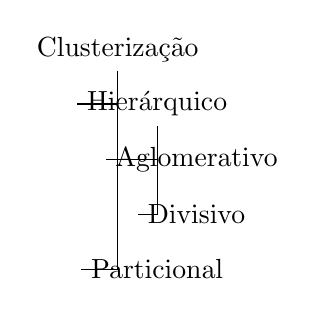
\begin{tikzpicture}[%
  grow via three points={one child at (0.5,-0.7) and
  two children at (0.5,-0.7) and (0.5,-1.4)},
  edge from parent path={(\tikzparentnode.south) |- (\tikzchildnode.west)}]
  \node {Clusterização}
    child { node {Hierárquico}
    	child { node {Aglomerativo}}
        child { node {Divisivo}}
    }	
    child [missing] {}				
    child [missing] {}	
    child { node {Particional}};
\end{tikzpicture}
\caption{Classificação das estratégias de clusterização} \label{tipos_clustering}
\end{figure}

\end{comment}

As estratégias de agrupamentos particionais buscam dividir um conjunto de elementos de entrada em um número fixo de \emph{clusters}. Estas estratégias utilizam pontos que se localizam no mesmo espaço dimensional dos elementos para representar cada um dos grupos formados \cite{leandro}. Estes pontos são denominados de protótipos e são usados como parâmetro de distância de um elemento ao \emph{cluster}.

\subsection{Agrupamento por Nuvens Dinâmicas}

O algoritmo de agrupamento por nuvens dinâmicas é um algoritmo iterativo de agrupamento particional que itera sobre passos de alocação de elementos e representação de \emph{clusters} até que o critério de parada seja alcançado.

O problema de otimização resolvido por este algoritmo é definido por \citeonline{carvalho} como se segue. Seja $\Omega$ o conjunto de $n$ objetos indexados por $i = 1, ..., n$ e descritos por $p$ variáveis quantitativas. Cada objeto $i$ é descrito por um vetor $\mathrm{x}_i = (x{^1_i}, ..., x{^p_i}) \in \Re^p$. O problema é achar a partição $P = (C_1, ..., C_k)$ de $\Omega$ em $K$ \emph{clusters} e o conjunto $Y = (y_1, ..., y_K)$ de exemplares que minimizam o critério de particionamento $g(P,Y)$ que mede a adequação entre os \emph{clusters} e seus representantes.

A inicialização do algoritmo se dá pela declaração inicial das partições e de seus respectivos protótipos como mostra o Algoritmo \ref{initialize}. Uma vez inicializado, o algoritmo busca encontrar a melhor alocação para os elementos de maneira que o critério de particionamento $g(P,Y)$ seja minimizado. Para tal, os elementos são alocados nos \emph{clusters} de acordo com suas proximidades aos exemplares \cite{carvalho}.

\begin{algorithm}[htb]
\caption{Função \emph{Initialize} que inicializa os \emph{K clusters}.}
\label{initialize}
	\begin{algorithmic}[1]
		\Function{initialize}{}
			\LeftTextComment{Escolha uma partição $(C_1, ..., C_K)$ de $\Omega$ ou escolha $K$ objetos diferentes $y_1, ..., y_K$ entre $\Omega$ e aloque cada objeto $i$ ao exemplar mais próximo para construir a partição inicial $(C_1, ..., C_K)$.			
			}
		\EndFunction
	\end{algorithmic}
\end{algorithm}

O Algoritmo \ref{representation} mostra que a eleição dos protótipos acontece através da verificação de qual elemento está mais próximo ao restante dos elementos, este elemento representará o centro do \emph{cluster} e por isso pode ser chamado de centroide. Em algumas configurações do algoritmo, o representante do \emph{cluster} pode ser calculado como a média de todos os elementos presentes naquele \emph{cluster}. O centroide de um \emph{cluster} poderá ser usado como parâmetro para o cálculo de distância de um elemento ao \emph{cluster}.

\begin{algorithm}[htb]
\caption{Função \emph{Representation} que elege os protótipos de cada \emph{cluster}.}
\label{representation}
	\begin{algorithmic}[1]
		\Function{representation}{}
			\For{$ k \gets 0; i<K; k++ $}
				\LeftTextComment{Calcule o exemplar $y_k$ }
			\EndFor			
		\EndFunction
	\end{algorithmic}
\end{algorithm}

O Algoritmo \ref{allocation} apresenta a função responsável por alocar os elementos em seus respectivos \emph{clusters}. Esta etapa do algoritmo de agrupamento por nuvens dinâmicas percorre todos os elementos averiguando o \emph{cluster} em que o elemento melhor se encaixa (menor distância) para que a melhor configuração seja estabelecida.

\begin{algorithm}[htb]
\caption{Função \emph{Allocation} que aloca os elementos.}
\label{allocation}
	\begin{algorithmic}[1]
		\Function{Allocation}{}
			\State $teste \gets 0$
			\For{$ i \gets 0; i<n; i++ $}
					\LeftTextComment{seja o \emph{cluster} $C_{k*}$ tal que $k* = min_{k=0,...,K} \ d^{k}_r (\mathrm{x}_i, \mathrm{y}_k)$}
					\If{$i \in C_k \quad E \quad k* \neq k $}
						\State $teste \gets 1$
						\State $C_{k*} \gets C_{k*} \cup \{i\}$
						\State $C_k \gets C_k \setminus \{i\}$
					\EndIf	
			\EndFor
			\State \Return \emph{teste}
		\EndFunction
	\end{algorithmic}
\end{algorithm}

A linha 2 do Algoritmo \ref{allocation} declara a variável que indica quando uma mudança na configuração dos \emph{clusters} for efetivada. Esta mudança é essencial para o algoritmo de agrupamento por nuvens dinâmicas, uma vez que esta indicará a necessidade de mais uma iteração do algoritmo.

O Algoritmo \ref{dynamicClustering} reúne as etapas apresentadas para contemplar a proposta do algoritmo de agrupamento. Uma vez que os \emph{clusters} são inicializados, o algoritmo itera pelas etapas de representação (\Call{Representation}{}) e alocação (\Call{Allocation}{}) até que nenhuma melhoria possa ser feita pela etapa de alocação.

\begin{algorithm}[htb]
\caption{Algoritmo de agrupamento por nuvens dinâmicas.}
\label{dynamicClustering}
	\begin{algorithmic}[1]
		\Function{dynamicClustering}{}
		
			\State $\Call{initialize}{}$
			\Repeat
				\State $\Call{representation}{}$
				\State $teste \gets \Call{allocation}{}$
			\Until {\emph{teste = 0}}
		\EndFunction
	\end{algorithmic}
\end{algorithm}

\section{Internet}
O avanço e estruturação das redes de computadores possibilitaram que várias aplicações que se baseiam na comunicação em redes surgissem. A \emph{INTERNET} refere-se a arquitetura de redes globais que estão interconectadas e se comunicam através de conjuntos de regras e protocolos. A \emph{INTERNET} usa funcionalidades relativamente simples com escalabilidade, eficiência e utilidade suficientes para resultarem em um espaço confiável \cite{www}.

A \emph{World Wide Web} (WWW) ou simplesmente \emph{Web} é uma das diversas aplicações de escala mundial que possibilitam que instituições e pessoas de todo o mundo estejam conectadas através da \emph{INTERNET}.

A \emph{World Wide Web} pode ser considerada um enorme sistema para acessar documentos ligados, que consiste em milhões de clientes e servidores. Servidores mantêm conjuntos de documentos, enquanto clientes fornecem a usuários uma interface de fácil utilização para apresentar e acessar esses documentos \cite{distribuidostanenbaum}.

O padrão \emph{Web} teve início no Laboratório Europeu de Física Nuclear (\emph{European Particle Physics Laboratory} - CERN), em Genebra, como um projeto que permitiria seu grupo de pesquisadores, numeroso e geograficamente disperso, acessar documentos compartilhados por meio de um sistema simples de hipertexto. Um documento podia ser qualquer coisa que pudesse ser representada no terminal do computador de um usuário \cite{distribuidostanenbaum}. 

O núcleo de um site \emph{Web} é formado por um processo que tem acesso a um sistema de arquivos local que armazena documentos. O modo mais simples de referenciar um documento é por meio de uma referência denominada localizador uniforme de recurso ou \emph{Uniform Resource Locator} (URL) \cite{distribuidostanenbaum}. Cada documento disponível na \emph{Web} possui um URL associado que será usado para que o serviço cliente tenha acesso a estes documentos.

A comunicação entre um \emph{browser} e um servidor se baseia no protocolo de transferência de hipertexto ou \emph{Hypertext Transfer Protocol} (HTTP). O protocolo HTTP foi originalmente projetado para transferência de conteúdo \emph{Web}, mas agora suporta a transferência de arquivos de qualquer tipo \cite{fundamentalsofmultimedia}.

O \emph{browser} ou navegador é a aplicação responsável por abstrair os procedimentos envolvidos na requisição e tratamento da resposta obtida. A Figura \ref{http} ilustra o procedimento em que um cliente realiza uma requisição HTTP e obtém uma resposta do servidor. Uma vez que a máquina cliente recebe uma resposta do servidor com o conteúdo esperado, o \emph{browser} analisa a resposta e apresenta o conteúdo do documento.

\begin{figure}[htb]
\begin{center}
  \centering
  \caption{Organização global de \emph{Website}.}
      \includegraphics[scale=0.6]{images/httpTanenbaum.png}
    
    \label{http}
  %\end{subfigure}
  
  \legend{\textbf{Fonte:} \citeonline{distribuidostanenbaum}.}
\end{center}

\end{figure}

%O conteúdo de uma resposta HTTP contém essencialmente trechos que demarcam e descrevem a estrutura de uma página \emph{Web}, estilo e comportamento. 
 
\subsection{HTML e CSS}
Uma página \emph{Web} é formada principalmente de código HTML, uma linguagem de marcação usada para indicar ao \emph{browser} como estruturar as páginas. HTML consiste em uma série de elementos usados para delimitar ou marcar diferentes partes do conteúdo para que sejam exibidos de maneira específica de acordo com o elemento indicado \cite{mdn}. Os elementos são delimitados por \emph{tags} que definem o início de um elemento no formato \emph{<tag>} e \emph{</tag>} que delimita o fim do elemento. 

Um documento HTML simples é dividido entre cabeçalho e corpo. O cabeçalho descreve as definições do documento que são interpretadas antes do processo de montagem do documento ser concluído. Estas definições incluem título da página, \emph{links} para recursos utilizados e outras informações que o autor desejar especificar. O corpo de uma página descreve a estrutura do documento e seu conteúdo. Estas estruturas podem ser parágrafos, tabelas, formulários, listas de itens e botões \cite{fundamentalsofmultimedia}.

O Código \ref{exemploHtml} mostra o exemplo de uma página simples HTML. As linhas 1 e 10 delimitam que o texto em seu interior é um código HTML, as 2 e 4 delimitam o cabeçalho da página, as 6 e 9 delimitam o corpo. No interior destes elementos, a linha 3 declara o título da página, a linha 7 declara o título do texto e a linha 8 declara um parágrafo. O resultado deste exemplo em um \emph{browser} é apresentado na Figura \ref{htmlExemploImagem}.

\lstinputlisting[caption={Exemplo de página HTML}, label={exemploHtml},language=HTML]{code/htmlExample.html}


Os elementos HTML podem conter atributos que adicionam informações extras sobre o elemento. Um atributo permite que um elemento específico passe a ter uma identificação que pode ser usada para estilizar este elemento. A estilização de uma página e de seus elementos é feita através da linguagem \emph{Cascading Style Sheets} (CSS). A linguagem CSS permite a customização de cores de texto e fundo dos elementos, fontes, tamanhos e espaçamentos entre \mbox{outros \cite{mdn}}.

\begin{figure}[htb]
\begin{center}
  \centering
  \caption{Código \ref{exemploHtml} apresentado no \emph{browser}.}
      \fbox{\includegraphics[scale=0.6]{images/htmlExemplo.png}}
    
    \label{htmlExemploImagem}
  
  \legend{\textbf{Fonte:} Autoria Própria.}
\end{center}

\end{figure}

\subsection{JavaScript} 
Os \emph{browsers} não se limitam apenas a apresentar as páginas \emph{Web} estáticas, eles permitem que os usuários interajam com páginas através da linguagem \emph{JavaScript}. Apesar do nome, \mbox{\emph{JavaScript}} e \emph{Java} são linguagens totalmente diferentes. A linguagem \emph{JavaScript} é uma linguagem de \emph{script} que é interpretada por um \emph{browser}, isto significa que os \emph{scripts} \emph{JavaScript} são executados por a máquina cliente sem a necessidade de passar por um compilador.\footnote{\emph{Script} é uma sequência de instruções a ser interpretada por um programa em vez de ser compilada.}

\emph{JavaScript} é uma linguagem de programação que permite a implementação de interações complexas nas páginas \emph{Web}. Ela permite a atualização de componentes HTML e regras CSS de maneira dinâmica e permite armazenar valores em variáveis, realizar operações em textos e executar ações em resposta a eventos que venham a acontecer na página \cite{mdn}. 

O Código \ref{exemploHtmlJS} é um exemplo de como \emph{JavaScript} pode interagir com HTML e CSS. Neste exemplo, o botão definido na linha 5 define o código \emph{JavaScript} a ser executado quando um evento de clique for detectado no botão. A ação declarada no atributo \emph{onclick} do botão HTML (\emph{document.getElementById('paragrafo').style.display = 'none'}) acessa o elemento HTML da linha 4 através do identificador definido no atributo \emph{id} e altera o atributo CSS \emph{display} para \emph{none} fazendo com que este fique invisível.

\lstinputlisting[caption={Exemplo de página HTML com código \emph{JavaScript} interagindo com CSS}, label={exemploHtmlJS},language=HTML]{code/htmlJavaScript.html}

Os códigos \emph{JavaScript} são executados por um processador de código \emph{JavaScript} contido no \emph{browser} depois que os códigos HTML e CSS são carregados. Isto porque os \emph{scripts} \emph{JavaScript} interagem com os componentes da página e precisam que eles estejam carregados.
 
\subsection{Disposição e Recuperação de Informações na Internet}
É fato que a \emph{Web} é um serviço democrático e dinâmico assim como o mundo virtual em geral. Com a popularização da \emph{INTERNET} e dos dispositivos digitais, artefatos multimídias dos mais diversos formatos são gerados a cada instante. Com isso, é comum que estas mídias sejam disponibilizadas na \emph{WWW} em \emph{Websites} dos mais diversos tipos.

Com o alto volume de dados sendo disponibilizados na \emph{INTERNET} nos mais variados formatos, a tarefa de encontrar ou recuperar uma informação de maneira não metódica é inviável pois os documentos disponibilizados não seguem qualquer ordem. É por isso que vários serviços como \emph{Google}, \emph{Yahoo} e \emph{Bing} se dispõem a realizar buscas na \emph{INTERNET} de maneira eficiente. O \citeonline{nms} indica que o motor de busca do \emph{Google} dominou cerca de 73\%  deste mercado.

O \emph{Google} é uma corporação dos Estados Unidos cuja missão é dominar o enorme volume de informações: ``\emph{organizar as informações do mundo e torná-las universalmente acessíveis e úteis}'' \cite{google}. 

Inaugurada em 1998, o \emph{Google} cresceu até ter uma fatia dominante do mercado de pesquisa na \emph{INTERNET} principalmente devido à eficiência de seu algoritmo. Desde seu sistema de produção inicial, até lidar com mais de 88 bilhões de pesquisas por mês (em 2010), seu principal mecanismo de busca nunca sofreu uma interrupção em todo esse tempo e seus usuários podem esperar resultados de consulta em torno de 0,2 segundos \cite{coulouris}.

A seguir é apresentada uma síntese de uma breve apresentação do serviço de busca do \emph{Google} feita por \citeonline{coulouris}. A função do mecanismo de busca do Google, assim como para qualquer mecanismo de pesquisa na \emph{Web}, é receber determinada consulta e retornar uma lista ordenada com os resultados mais relevantes que satisfazem essa consulta, pesquisando o conteúdo na \emph{Web}. O mecanismo de busca do \emph{Google} consiste em um conjunto de serviços para esquadrinhar a \emph{Web} e indexar e classificar as páginas descobertas. 

A tarefa de esquadrinhar refere-se a uma análise minuciosa do conteúdo da \emph{Web}. Esta tarefa analisa as páginas recursivamente coletando todos os \emph{links} que apontam para outras páginas para que estas também sejam esquadrinhados por este procedimento. O objetivo é mapear todo o conteúdo disponível na \emph{INTERNET} para que seja gerado um índice de palavras ou termos que serão usados como parâmetros de busca.

O índice de palavras gerado adota critérios de comparação e ordenação como número de ocorrências, posição no documento e tamanho da fonte usada. Além do índice de palavras, o motor de busca mantém um índice de \emph{links} que monitora as páginas que ligam a um determinado \emph{Website}. Este índice de \emph{links} é usado por o algoritmo \emph{PageRank} que classifica as páginas de acordo com sua relevância. 

%\subsection{Recuperação de Imagens}

%\subsubsection{Motores de Busca}

%\subsubsection{Google}



%\subsection{Aplicação}


% ---

% ---
% Capitulo de desenvolvimento
% ---
\chapter{Extensão para o \emph{Mozilla Firefox}}
Este capítulo trata da aplicação do algoritmo de agrupamento por nuvens dinâmicas para o refinamento de buscas por imagens na \emph{INTERNET} usando o motor de busca do \emph{Google}. O serviço do \emph{Google} de pesquisa oferece por si uma organização dos resultados em grupos. A diferença da organização do \emph{Google} para a organização proposta é que enquanto os resultados e a busca têm como parâmetro de diferenciação o texto associado aos componentes de busca, este trabalho propõe que a disposição dos resultados seja feita com base no conteúdo das imagens. O fluxo de passos executados pela extensão é representado na Figura \ref{fluxo_aplicacoes}.

% Define block styles
\tikzstyle{decision} = [diamond, draw, fill=blue!20, 
    text width=4.5em, text badly centered, node distance=3cm, inner sep=0pt]
\tikzstyle{block} = [rectangle, draw, fill=blue!20, 
    text width=5em, text centered, rounded corners, minimum height=4em]
\tikzstyle{line} = [draw, -latex']
\tikzstyle{cloud} = [draw, ellipse,fill=red!20, node distance=3cm,
    minimum height=2em]
    
\begin{figure}[htb]
\caption{\label{fluxo_aplicacoes}Fluxograma de execução da aplicação.}
\begin{center}
\begin{tikzpicture}[node distance = 2cm, auto]
    % Place nodes
    \node [block] (init) {Início};
    \node [block, below of=init] (identify) {Carrega Imagens};
    \node [block, right of=identify, node distance=3cm] (descritores) {Gera descritores};
    \node [block, right of=descritores, node distance=3cm] (dynamicClustering) {Agrupamento};
    \node [block, right of=dynamicClustering, node distance=3cm] (resultados) {Exibe Resultados};
    \node [block, above of=resultados] (fim) {Fim};
    % Draw edges
    \path [line] (init) -- (identify);
    \path [line] (identify) -- (descritores);
    \path [line] (descritores) -- (dynamicClustering);
    \path [line] (dynamicClustering) -- (resultados);
    \path [line] (resultados) -- (fim);
    
\end{tikzpicture}
\end{center}
\legend{\textbf{Fonte:} Autoria Própria.}
\end{figure}

\begin{comment}
\begin{figure}[htb]
\caption{\label{fluxo_aplicacoes}Fluxograma de Execução das Aplicações.}
\begin{center}
\includegraphics[width=450px]{images/fluxo1.png}
\end{center}
\legend{\textbf{Fonte:} Autoria Própria.}
\end{figure}
\end{comment}

\section{Aplicação}
A extensão do \emph{Mozilla Firefox} foi desenvolvida em \emph{JavaScript} e não altera o modo com que o usuário navega na \emph{INTERNET}, então para que a execução do código seja iniciada é necessário que o usuário acesse a página de resultados de pesquisas de imagens do \emph{Google}. O \emph{Mozilla Firefox} foi escolhido por se tratar de um navegador de código aberto desenvolvido sem fins lucrativos, além disso, o \emph{Mozilla Firefox} é adotado como navegador padrão na maioria dos sistemas operacionais de código aberto e de licença livre.

O Algoritmo \ref{algo_base} é um esboço do que é feito pela aplicação proposta. A extensão verifica a página que está sendo acessada a cada página carregada no navegador, quando a página em questão é a página específica, a extensão exibe uma caixa de diálogo \emph{JavaScript} para que o usuário informe o número de \emph{clusters} desejados como mostra a Figura \ref{input}. De maneira semelhante, o usuário escolhe o descritor a ser usado pelo algoritmo. Isto feito, as imagens são carregadas, os descritores são gerados, o algoritmo executado e o resultado apresentado na própria página.

As imagens que são mostradas como resultado de uma busca por imagens na página do \emph{Google} são os parâmetros de entrada do código. Assim como a maioria dos \emph{Websites} na \emph{INTERNET} as páginas de resultados de buscas do \emph{Google} são compostas por componentes HTML, CSS e códigos \emph{JavaScript}. 

\begin{algorithm}[htb]
\caption{Aplicação do algoritmo de agrupamento por nuvens dinâmicas em imagens da página de resultados do \emph{Google}.}
\label{algo_base}
	\begin{algorithmic}[1]
		\Function{agruparImagens}{\emph{document}}
			\If{\Call{isResultPage}{\emph{document}}}
				\State $imagens \gets document.getElementsByClassName("rg\_ic rg\_i")$
				\State $descritores \gets \Call{GerarDescritores}{\emph{imagens}}$
				\State $clusters \gets \Call{dynamicClustering}{\emph{descritores}}$
				\State $\Call{showResults}{\emph{clusters}}$
			\EndIf
		\EndFunction
	\end{algorithmic}
\end{algorithm}

\begin{figure}[htb]
\begin{center}
  %\caption{Imagem colorida ampliada.}
  %\begin{subfigure}[b]{0.6\textwidth}
  \centering
  \caption{Caixa de diálogo para entrada do número de grupos desejado.}
      \includegraphics[scale=0.6]{images/input.png}
    
    \label{input}
  %\end{subfigure}
  
  \legend{\textbf{Fonte:} Autoria Própria.}
\end{center}

\end{figure}

A obtenção das imagens da página de resultados do \emph{Google} é possível através de \emph{scripts} \emph{JavaScript} que são capazes de acessar os elementos HTML e suas propriedades. Como descrito anteriormente, os códigos HTML são organizados por componentes e divisores e estes são úteis para exibir o conteúdo da página de maneira estilizada para cada componente e divisão.

O Código \ref{exemplo_simplificado} é um exemplo simplificado de um componente que referencia uma imagem retornada de uma busca. A linha dois do código define o componente que contém a URL da imagem, mas é só na linha três que o componente, que de fato exibe a imagem, é descrito. A imagem referenciada por este componente é representada por uma codificação base 64 e este código está na propriedade \emph{src} do componente da imagem.  
\lstinputlisting[caption={Exemplo Simplificado de Componente \emph{HTML}}, label={exemplo_simplificado},language=HTML]{code/htmlImageExample.html}

Se habilitado no \emph{browser} pelo usuário, os códigos \emph{JavaScript} das páginas na \emph{Web} serão executados. Estes códigos podem estar contidos na própria página a partir dos desenvolvedores da página ou podem ser inseridos de acordo com que as páginas são carregadas no navegador, isto acontece através da ação do próprio navegador ao suportar as extensões.

Sempre que uma página é completamente carregada, um evento é disparado e pode ser identificado por aplicações \emph{JavaScript}. Quando isto acontece, a aplicação desenvolvida neste trabalho varre os elementos HTML em busca de componentes que são da classe \emph{rg\_ic rg\_i}. Esta classe identifica as imagens que são retornadas da busca como mostra o Código \ref{exemplo_simplificado}. A extensão identifica que a página atual contém resultados de busca através do Algoritmo \ref{verifica_pagina}.
\begin{algorithm}[htb]
\caption{Função que verifica se página em questão é página de resultados da busca por imagens.}
\label{verifica_pagina}
	\begin{algorithmic}[1]
	\Function{isResultPage}{\emph{document}}
		\State $imagens \gets document.getElementsByClassName(``rg\_ic\ rg\_i")$
		\State $imagesLength \gets imagens.length$
		\If{$imagensLength > 0$}
			\State \Return $true$
		\Else
			\State \Return $false$
		\EndIf
	\EndFunction
	\end{algorithmic}
\end{algorithm}

Uma vez que as imagens, que serão a entrada do algoritmo são identificadas na página, o algoritmo segue para a fase de geração dos descritores. Nesta fase, a geração do descritor acontece através de um código em \emph{JavaScript} que interage com o componente HTML \emph{canvas} que permite o acesso aos \emph{pixels} das imagens. 

A aplicação suporta o uso dos dois descritores apresentados. A razão para utilização de dois descritores diferentes é que estes são usados pelo algoritmo de agrupamento e dependendo da escolha do descritor, o algoritmo pode apresentar melhor ou pior qualidade em seus resultados.

\begin{comment}
Duas versões da aplicação foram desenvolvidas, as duas versões variam quanto ao uso do descritor. Uma versão utiliza os histogramas das imagens como descritores e outra versão utiliza o autovetor dominante da imagem como descritor. A razão para utilização de dois descritores diferentes é que estes são usados por o algoritmo de agrupamento e dependendo da escolha do descritor, o algoritmo pode apresentar melhor ou pior qualidade em seus resultados.
\end{comment}

\section{Carregamento de Imagens e Geração de Descritores}
A página de busca de imagens do \emph{Google} pode retornar diversas imagens que vão sendo exibidas de acordo com que o usuário rola a página para baixo. Os componentes que contém as imagens indicam se a imagem está carregada ou não através do atributo src que significa \emph{source} e indica a origem da imagem, que pode ser uma URL ou o próprio conteúdo codificado da imagem. 

Uma vez que a extensão identifica que o documento carregado é identificado como a página de resultados de busca, a aplicação filtra as imagens que foram carregadas com base no atributo \emph{source} descrito anteriormente. Estas imagens são adicionadas a uma estrutura que referenciará as imagens carregadas.

Quando o descritor em questão é o autovetor, a aplicação varre as imagens identificando as imagens não quadradas, ou seja imagens cuja altura e largura são diferentes, para que estas sejam transformadas em imagens quadradas a fim de que seja possível calcular o autovetor dominante da imagem em questão. Isto é feito adicionando elementos à dimensão que possui menos elementos. Por exemplo, seja a imagem $A_{n \times m}$ de forma que $n > m$, neste caso a imagem possui mais linhas que colunas e por isso $n - m$ colunas serão adicionadas para que a imagem seja quadrada.

Uma vez que a etapa de carregamento das imagens é finalizada, a etapa de geração de descritores varre todas as imagens carregadas acessando os \emph{pixels} através do componente \emph{canvas}. O \emph{canvas} é um componente HTML usado para desenhar gráficos e animações via \emph{scripts}. O HTML \emph{canvas} oferece uma série de opções para gerenciamento da cena. 

O \emph{canvas} possui uma referência ao objeto \emph{context} que oferece métodos para o gerenciamento do \emph{canvas}. É possível referenciar o \emph{context} através do método \emph{getContext()} e assim acessar métodos como o \emph{drawImage()} que desenha um componente de imagem, vídeo ou próprio \emph{canvas} passado como parâmetro. 

Este componente suporta a exibição de imagens suportadas pelo próprio navegador, desta forma é desnecessário qualquer tipo de tratamento ou conversão quanto aos tipos de imagens. Com isso, é possível acessar cada \emph{pixel} de qualquer imagem que esteja sendo exibida na página e assim calcular o descritor em questão da respectiva imagem.

\section{Agrupamento e Exibição dos Resultados}
O Algoritmo \ref{dynamicClustering} é implementado em \emph{JavaScript} e o mesmo código é usado independentemente do tipo de descritor em questão. Isto porquê uma vez que os descritores são gerados, o algoritmo só precisa calcular as distâncias. A aplicação armazena o resultado do algoritmo em uma matriz, de forma que a quantidade de linhas representa o número de \emph{clusters} e as colunas representam os elementos.

\begin{figure}[htb]
\begin{center}
  %\caption{Imagem colorida ampliada.}
  %\begin{subfigure}[b]{0.6\textwidth}
  \centering
  \caption{Resultado de busca.}
      \fbox{\includegraphics[width=\textwidth]{images/tomate.png}}
    
    \label{resultadoBusca}
  %\end{subfigure}
  
  \legend{\textbf{Fonte:} \citeonline{google0}.}
\end{center}

\end{figure}

A apresentação dos resultados acontece na própria página de resultados. Algumas páginas de resultados do \emph{Google} possuem um componente HTML que exibe grupos relacionados a busca feita. A Figura \ref{resultadoBusca} mostra a região que classifica a busca por tomate em Jitomate Vs, Verde, Jitomate e Caricatura. Esta mesma região será duplicada na página para exibir os resultados do algoritmo. Uma vez que esta região é copiada na página, a aplicação substitui as imagens pelas imagens agrupadas pela aplicação como mostra a Figura \ref{tomateCluster}.

\begin{figure}[htb]
\begin{center}
  %\caption{Imagem colorida ampliada.}
  %\begin{subfigure}[b]{0.6\textwidth}
  \centering
  \caption{Exibição do resultado do algoritmo na própria página.}
      \fbox{\includegraphics[width=\textwidth]{images/tomateCluster.png}}
    
    \label{tomateCluster}
  %\end{subfigure}
  
  \legend{\textbf{Fonte:} \citeonline{google0}.}
\end{center}

\end{figure}
% ---


% ---
% Capitulo de resultados
% ---
\chapter{Resultados}

Este capítulo apresenta os resultados obtidos com a aplicação desenvolvida e uma discussão acerca destes. A análise dos resultados será feita através da comparação dos dois descritores implementados. Antes de apresentar os resultados com imagens provenientes de uma busca, serão apresentados resultados do algoritmo em uma página de testes. As páginas de testes foram usadas como guias de ajustes e validação visual do algoritmo proposto.

A Tabela \ref{paginaTeste} apresenta as imagens presentes em uma página de teste. Apesar de todas estas imagens serem diferentes, as características que elas carregam são semelhantes entre algumas. As imagens da linha um são de tomates apresentados em diferentes ângulos em uma imagem de fundo próximo ao branco. Semelhantemente, a linha dois apresenta imagens de balões com fundo azul não necessariamente na mesma tonalidade. 

\begin{table}[h]
    \begin{center}
      \caption{Imagens de página de teste.}
\begin{tabular}{ |>{\centering\arraybackslash}m{5cm} | >{\centering\arraybackslash}m{5cm} | >{\centering\arraybackslash}m{5cm} | } 
\hline
   \begin{subfigure}[b]{5cm}
   \centering
   \includegraphics[width=5cm,height=4cm,keepaspectratio,trim=0 0 0 -5]{images/paginaTeste/tomate1.jpg}
   \caption*{1}
  \end{subfigure}
   &
    \begin{subfigure}[b]{5cm}
  \centering
   \includegraphics[width=5cm,height=4cm,keepaspectratio,trim=0 0 0 -5]{images/paginaTeste/tomate2.jpg}
   \caption*{2}
  \end{subfigure}
   & 
    \begin{subfigure}[b]{5cm}
  \centering
   \includegraphics[width=5cm,height=4cm,keepaspectratio,trim=0 0 0 -5]{images/paginaTeste/tomate3.jpg}
   \caption*{3}
  \end{subfigure} \\ 
 \hline
   \begin{subfigure}[b]{5cm}
  \centering
   \includegraphics[width=5cm,height=4cm,keepaspectratio,trim=0 0 0 -5]{images/paginaTeste/balao1.jpg}
   \caption*{4}
  \end{subfigure}
   &
   \begin{subfigure}[b]{5cm}
  \centering
   \includegraphics[width=5cm,height=4cm,keepaspectratio,trim=0 0 0 -5]{images/paginaTeste/balao2.jpg}
	\caption*{5}
   \end{subfigure}
   & 
   \begin{subfigure}[b]{5cm}
  \centering
    \includegraphics[width=5cm,height=4cm,keepaspectratio,trim=0 0 0 -5]{images/paginaTeste/balao3.jpg}
    \caption*{6}
  \end{subfigure} \\ 
 
 \hline
\end{tabular}
\label{paginaTeste}
\legend{\textbf{Fonte:} \citeonline{google0, google1}.}
\end{center}
\end{table}

A matriz de distâncias entre as imagens calculada através dos autovetores dominantes é apresentada na Tabela \ref{matrizDistanciaAutoVetores} e a calculada através dos histogramas é apresentada na Tabela \ref{matrizDistanciaHistogramas}. As células destacadas indicam os dois menores valores, ou seja as duas imagens mais próximas.

\begin{sidewaystable}[pht!]

\centering
    \caption{Matriz de distâncias - Autovetores Dominantes.}
\begin{tabular}{|l|l|l|l|l|l|l|}
        \hline
         & 1 & 2  & 3 & 4 & 5 & 6   \\ \hline
        1   &  0 & \cellcolor{blue!25}0.7903890183496494 & \cellcolor{blue!25}1.267739792773765 & 1.5707963267948966 &  1.5707960225553694 & 1.5707963267027802\\ 
        \hline
        2   &  \cellcolor{blue!25}0.7903890183496494& 0& \cellcolor{blue!25}1.1557908824986878& 1.5707963267948966 &  1.5707962171666512 & 1.5707963266958864\\
        \hline 
        3   &  \cellcolor{blue!25}1.267739792773765 & \cellcolor{blue!25}1.1557908824986878 & 0 & 1.5707963267948966 &  1.5632618141959285 & 1.5707963267041545\\ 
        \hline
        4   &  1.5707963267948966 & 1.5707963267948966 & 1.5707963267948966 & 0 &  \cellcolor{blue!25}1.5707962924625574 & \cellcolor{blue!25}1.5707804758766788\\ 
        \hline
        5   &  1.5707960225553694 & 1.5707962171666512 & 1.5632618141959285 & \cellcolor{blue!25}1.5707962924625574 &  0 & \cellcolor{blue!25}1.5707679774026786\\ 
        \hline
        6   &  1.5707963267027802 & 1.5707963266958864 & 1.5707963267041545 & \cellcolor{blue!25}1.5707804758766788 &  \cellcolor{blue!25}1.5707679774026786 & 0\\ 
        \hline
    \end{tabular}
\label{matrizDistanciaAutoVetores}
    \legend{\textbf{Fonte}: Autoria Própria}

\centering
    \caption{Matriz de distâncias - Histogramas.}
\begin{tabular}{|l|l|l|l|l|l|l|}
        \hline
         & 1 & 2  & 3 & 4 & 5 & 6   \\ \hline
        1   &  0 & \cellcolor{blue!25}0.5756075471698113 & \cellcolor{blue!25}0.5971680480729381 & 0.6794026881720429 &  0.6567888888888888 & 0.7045434782608694\\ 
        \hline
        2   &  \cellcolor{blue!25}0.5756075471698113 & 0& \cellcolor{blue!25}0.42156721584082& 0.6947065074051536 &  0.7187795946890287 & 0.7458547990155866\\ 
        \hline
        3   &  \cellcolor{blue!25}0.5971680480729381 & \cellcolor{blue!25}0.42156721584082 & 0 & 0.6477030282876355 &  0.588672665039677 & 0.6363063718865803\\ 
        \hline
        4   &  0.6794026881720429 & 0.6947065074051536 & 0.6477030282876355 & 0 &  \cellcolor{blue!25}0.4964178912783750 & \cellcolor{blue!25}0.2739817671809256\\
        \hline 
        5   &  0.6567888888888888 & 0.7187795946890287 & 0.588672665039677 & \cellcolor{blue!25}0.4964178912783750 &  0 & \cellcolor{blue!25}0.3671427536231884\\ 
        \hline
        6   &  0.7045434782608694 & 0.7458547990155866 & 0.6363063718865803 & \cellcolor{blue!25}0.2739817671809256 &  \cellcolor{blue!25}0.3671427536231884 & 0\\ 
        \hline
    \end{tabular}
\label{matrizDistanciaHistogramas}
    \legend{\textbf{Fonte}: Autoria Própria}

\end{sidewaystable}

\pagebreak

Como esperado, o algoritmo de agrupamento por nuvens dinâmicas alocou todas as imagens da linha um (tomates) em um grupo e consequentemente as imagens da linha dois (balões) foram alocadas em um grupo distinto.

A seguir são apresentados os resultados da aplicação e da busca pelas palavras chaves, casa, lentilha e gato. As Tabelas \ref{chaves}, \ref{casa}, \ref{lentilha} e \ref{gato} apresentam as imagens na ordem inicial disposta na página do \emph{Google}. As outras tabelas apresentam os resultados obtidos através da extensão e dispõem as imagens de acordo com as alocações de forma que cada agrupamento é identificado por uma cor de fundo. Cada imagem é identificada por um número e os protótipos de cada grupo são identificados pelo número de identificação entre colchetes.

A Tabela \ref{chavesAutoVetor} apresenta o conjunto de imagens da Tabela \ref{chaves} organizado em três grupos. É possível observar que neste conjunto existem imagens similares como 1, 10, 13, 11, 21 que foram alocadas no mesmo grupo. De maneira semelhante, as imagens 0 e 8 foram alocadas no mesmo grupo. Entretanto, também é possível observar que as imagens 25 e 32 foram alocadas em grupos diferentes sendo que elas são visualmente parecidas, apesar de uma ser colorida e a outra não. Isto pode acontecer devido a diferenças como contraste por exemplo.

O resultado para o conjunto de imagens da Tabela \ref{chaves} em três grupos usando os histogramas como descritores está disposto na Tabela \ref{chavesHistograma}. Com o uso de histogramas como descritores, parecem mais heterogêneos se comparados aos grupos da Tabela \ref{chavesAutoVetor}. Desta forma, para este conjunto de dados, o uso dos autovetores dominantes parece mais adequado.

As imagens da Tabela \ref{lentilha} apresentam o conjunto de imagens obtido na pesquisa pela palavra lentilha. Este conjunto foi organizado em quatro grupos. Neste conjunto é possível observar várias imagens com regiões das cores marrom, branca e bege. Os resultados usando os autovetores dominantes são apresentados na Tabela \ref{lentilhaAutoVetor} e os resultados usando os histogramas estão na Tabela \ref{histogramas}.

O uso dos histogramas pareceu mais adequado para o conjunto de dados da Tabela \ref{lentilha} uma vez que a Tabela \ref{lentilhaHistograma} apresenta imagens melhores distribuídas de acordo com os aspectos visuais. No grupo um é possível ver imagens com predominância do branco e com cores concentradas no centro das imagens enquanto que o grupo dois apresenta imagens com cores mais distribuídas em meio ao branco assim como o grupo quatro. O grupo três concentra as imagens com regiões de cor marrom representadas pela imagem 26 que é o protótipo do grupo.

As imagens da Tabela \ref{casa} foram divididas em cinco grupos. Neste conjunto de dados é possível observar algumas imagens com características visualmente semelhantes, como as imagens 0, 2, 5, 6, 10, 11, 16, 30, 31, 32 que possuem fundo branco. Além dessas imagens é possível observar que apesar de algumas imagens não possuírem fundo branco, têm o branco predominando.

A Tabela \ref{casaAutoVetor} mostra os resultados da aplicação ao usar os autovetores dominantes como descritores. É possível observar que o primeiro grupo é homogêneo, mas poderia incluir outras imagens com as mesmas características como 16, 6, 2, 5, 10 e 30. Os elementos do segundo grupo parecem similares ao possuírem regiões verdes e regiões escuras. O terceiro grupo apresenta o elemento 28 que visualmente se encaixaria na característica tida como dominante do grupo dois. Apesar disso, as outras imagens do grupo se assemelham assim como as imagens dos próximos grupos.

A Tabela \ref{casaHistograma} apresenta os resultados usando os histogramas como descritores e assim como na Tabela \ref{casaAutoVetor}, algumas imagens com características predominantes brancas foram agrupadas em grupos diferentes. Entretanto isso não significa que os grupos estão heterogêneos como em alguns grupos dos resultados do outro descritor, mas que os grupos 1, 3 e 5 são semelhantes. Os grupos dois e quatro são homogêneos, o dois ao apresentar claramente imagens predominantemente com regiões escuras não encontradas em outras imagens do conjunto.

O conjunto de imagens da Tabela \ref{gato} apresenta o conjunto de imagens obtidas através da busca por gato que foi dividido em seis grupos. Para este conjunto, os resultados usando os autovetores dominantes e histogramas estão dispostos na Tabela \ref{gatoAutoVetor} e Tabela \ref{gatoHistograma} respectivamente.

Para o conjunto de dados da Tabela \ref{gato} os resultados com os autovetores dominantes se apresentaram mais satisfatórios se comparados aos resultados do outro descritor. O fato é que os resultados da Tabela \ref{gatoHistograma} não se apresentam criteriosos nas divisões apresentadas enquanto que os resultados da Tabela \ref{gatoAutoVetor} estão melhores distribuídos. 

O grupo um da Tabela \ref{gatoAutoVetor} apresenta imagens com aspectos mais neutros se comparadas as outras imagens do mesmo conjunto, mas é possível observar que o restante dos grupos apresenta resultados mais semelhantes. O grupo dois contém imagens com tons de cinza com baixo contraste, em contrapartida o grupo cinco dispõe de imagens com mais contraste. O grupo quatro destes resultados se destaca ao ter todas as imagens com gatos alaranjados. Além do grupo quatro, o grupo seis também se mostra homogêneo ao dispor de imagens de gatos ao centro com fundo predominantemente branco.

\newpage
\begin{table}[h]
    \begin{center}
      \caption{Imagens de página de pesquisa - Chaves.}
\begin{tabular}{ |>{\centering\arraybackslash}m{4.9cm} | >{\centering\arraybackslash}m{4.9cm} | >{\centering\arraybackslash}m{4.9cm} | } 
\hline
	\grbox{
   \begin{subfigure}[b]{5cm}
   \centering
   \includegraphics[width=5cm,height=2cm,keepaspectratio,trim=0 0 0 -5]{images/chaves/0.jpeg}
  \end{subfigure}}{0}
   &
   \grbox{
    \begin{subfigure}[b]{5cm}
  \centering
   \includegraphics[width=5cm,height=2cm,keepaspectratio,trim=0 0 0 -5]{images/chaves/1.jpeg}
  \end{subfigure}}{1}
   & 
   \grbox{
    \begin{subfigure}[b]{5cm}
  \centering
   \includegraphics[width=5cm,height=2cm,keepaspectratio,trim=0 0 0 -5]{images/chaves/2.jpeg}
  \end{subfigure}}{2} \\ 
 \hline
 \grbox{
   \begin{subfigure}[b]{5cm}
  \centering
   \includegraphics[width=5cm,height=2cm,keepaspectratio,trim=0 0 0 -5]{images/chaves/3.jpeg}
  \end{subfigure}}{3}
   &
   \grbox{
   \begin{subfigure}[b]{5cm}
  \centering
   \includegraphics[width=5cm,height=2cm,keepaspectratio,trim=0 0 0 -5]{images/chaves/4.jpeg}
   \end{subfigure}}{4}
   & 
   \grbox{
   \begin{subfigure}[b]{5cm}
  \centering
    \includegraphics[width=5cm,height=2cm,keepaspectratio,trim=0 0 0 -5]{images/chaves/5.jpeg}
  \end{subfigure}}{5} \\ 
   \hline
   \grbox{
   \begin{subfigure}[b]{5cm}
  \centering
   \includegraphics[width=5cm,height=2cm,keepaspectratio,trim=0 0 0 -5]{images/chaves/6.jpeg}
   \end{subfigure}}{6}
   &
   \grbox{
   \begin{subfigure}[b]{5cm}
  \centering
   \includegraphics[width=5cm,height=2cm,keepaspectratio,trim=0 0 0 -5]{images/chaves/7.jpeg}
   \end{subfigure}}{7}
   & 
   \grbox{
   \begin{subfigure}[b]{5cm}
  \centering
    \includegraphics[width=5cm,height=2cm,keepaspectratio,trim=0 0 0 -5]{images/chaves/8.jpeg}
  \end{subfigure}}{8} \\ 
   \hline
   \grbox{
   \begin{subfigure}[b]{5cm}
  \centering
   \includegraphics[width=5cm,height=2cm,keepaspectratio,trim=0 0 0 -5]{images/chaves/9.jpeg}
  \end{subfigure}}{9}
   &
   \grbox{
   \begin{subfigure}[b]{5cm}
  \centering
   \includegraphics[width=5cm,height=2cm,keepaspectratio,trim=0 0 0 -5]{images/chaves/10.jpeg}
   \end{subfigure}}{10}
   & 
   \grbox{
   \begin{subfigure}[b]{5cm}
  \centering
    \includegraphics[width=5cm,height=2cm,keepaspectratio,trim=0 0 0 -5]{images/chaves/11.jpeg}
  \end{subfigure}}{11} \\ 
   \hline
   \grbox{
   \begin{subfigure}[b]{5cm}
  \centering
   \includegraphics[width=5cm,height=2cm,keepaspectratio,trim=0 0 0 -5]{images/chaves/12.jpeg}
  \end{subfigure}}{12}
   &
   \grbox{
   \begin{subfigure}[b]{5cm}
  \centering
   \includegraphics[width=5cm,height=2cm,keepaspectratio,trim=0 0 0 -5]{images/chaves/13.jpeg}
   \end{subfigure}}{13}
   & 
   \grbox{
   \begin{subfigure}[b]{5cm}
  \centering
    \includegraphics[width=5cm,height=2cm,keepaspectratio,trim=0 0 0 -5]{images/chaves/14.jpeg}
  \end{subfigure}}{14} \\ 
   \hline
   \grbox{
   \begin{subfigure}[b]{5cm}
  \centering
   \includegraphics[width=5cm,height=2cm,keepaspectratio,trim=0 0 0 -5]{images/chaves/15.jpeg}
  \end{subfigure}}{15}
   &
   \grbox{
   \begin{subfigure}[b]{5cm}
  \centering
   \includegraphics[width=5cm,height=2cm,keepaspectratio,trim=0 0 0 -5]{images/chaves/16.jpeg}
   \end{subfigure}}{16}
   & 
   \grbox{
   \begin{subfigure}[b]{5cm}
  \centering
    \includegraphics[width=5cm,height=2cm,keepaspectratio,trim=0 0 0 -5]{images/chaves/17.jpeg}
  \end{subfigure}}{17} \\ 
   \hline
   \grbox{
   \begin{subfigure}[b]{5cm}
  \centering
   \includegraphics[width=5cm,height=2cm,keepaspectratio,trim=0 0 0 -5]{images/chaves/18.jpeg}
  \end{subfigure}}{18}
   &
   \grbox{
   \begin{subfigure}[b]{5cm}
  \centering
   \includegraphics[width=5cm,height=2cm,keepaspectratio,trim=0 0 0 -5]{images/chaves/19.jpeg}
   \end{subfigure}}{19}
   & 
   \grbox{
   \begin{subfigure}[b]{5cm}
  \centering
    \includegraphics[width=5cm,height=2cm,keepaspectratio,trim=0 0 0 -5]{images/chaves/20.jpeg}
  \end{subfigure}}{20} \\ 
   \hline
   \grbox{
   \begin{subfigure}[b]{5cm}
  \centering
   \includegraphics[width=5cm,height=2cm,keepaspectratio,trim=0 0 0 -5]{images/chaves/21.jpeg}
  \end{subfigure}}{21}
   &
   \grbox{
   \begin{subfigure}[b]{5cm}
  \centering
   \includegraphics[width=5cm,height=2cm,keepaspectratio,trim=0 0 0 -5]{images/chaves/22.jpeg}
   \end{subfigure}}{22}
   & 
   \grbox{
   \begin{subfigure}[b]{5cm}
  \centering
    \includegraphics[width=5cm,height=2cm,keepaspectratio,trim=0 0 0 -5]{images/chaves/23.jpeg}
  \end{subfigure}}{23} \\
 \hline
 \grbox{
 \begin{subfigure}[b]{5cm}
  \centering
   \includegraphics[width=5cm,height=2cm,keepaspectratio,trim=0 0 0 -5]{images/chaves/24.jpeg}
  \end{subfigure}}{24}
   &
   \grbox{
   \begin{subfigure}[b]{5cm}
  \centering
   \includegraphics[width=4.2cm,height=2cm,keepaspectratio,trim=0 0 0 -5]{images/chaves/25.jpeg}
   \end{subfigure}}{25}
   & 
   \grbox{
   \begin{subfigure}[b]{5cm}
  \centering
    \includegraphics[width=5cm,height=2cm,keepaspectratio,trim=0 0 0 -5]{images/chaves/26.jpeg}
  \end{subfigure}}{26} \\
 \hline
 \grbox{
 \begin{subfigure}[b]{5cm}
  \centering
   \includegraphics[width=5cm,height=2cm,keepaspectratio,trim=0 0 0 -5]{images/chaves/27.jpeg}
  \end{subfigure}}{27}
   &
   \grbox{
   \begin{subfigure}[b]{5cm}
  \centering
   \includegraphics[width=5cm,height=2cm,keepaspectratio,trim=0 0 0 -5]{images/chaves/28.jpeg}
   \end{subfigure}}{28}
   & 
   \grbox{
   \begin{subfigure}[b]{5cm}
  \centering
    \includegraphics[width=5cm,height=2cm,keepaspectratio,trim=0 0 0 -5]{images/chaves/29.jpeg}
  \end{subfigure}}{29} \\
 \hline
 \grbox{
 \begin{subfigure}[b]{5cm}
  \centering
   \includegraphics[width=5cm,height=2cm,keepaspectratio,trim=0 0 0 -5]{images/chaves/30.jpeg}
  \end{subfigure}}{30}
   &
   \grbox{
   \begin{subfigure}[b]{5cm}
  \centering
   \includegraphics[width=5cm,height=2cm,keepaspectratio,trim=0 0 0 -5]{images/chaves/31.jpeg}
  \end{subfigure}}{31}
   &
   \grbox{
   \begin{subfigure}[b]{5cm}
  \centering
   \includegraphics[width=4.2cm,height=2cm,keepaspectratio,trim=0 0 0 -5]{images/chaves/32.jpeg}
  \end{subfigure}}{32}  \\
 \hline
\end{tabular}
\label{chaves}
\legend{\textbf{Fonte:} \citeonline{google2}.}
\end{center}
\end{table}

\newpage

\colorlet{cluster1}{blue!25}
\colorlet{cluster2}{gray}
\definecolor{cluster3}{rgb}{0.88,1,1}
\begin{table}[h]
    \begin{center}
      \caption{Autovetor - Resultado do conjunto chaves em 3 grupos.}
\begin{tabular}{ |>{\centering\arraybackslash}m{4.9cm} | >{\centering\arraybackslash}m{4.9cm} | >{\centering\arraybackslash}m{4.9cm} | } 
	\hline
	\cellcolor{cluster1}
	\grbox{
   \begin{subfigure}[b]{5cm}
   \centering
   \includegraphics[width=5cm,height=2cm,keepaspectratio,trim=0 0 0 -5]{images/chaves/0.jpeg}
  \end{subfigure}}{0}
   &
   \cellcolor{cluster1}
   \grbox{
    \begin{subfigure}[b]{5cm}
  \centering
   \includegraphics[width=5cm,height=2cm,keepaspectratio,trim=0 0 0 -5]{images/chaves/8.jpeg}
  \end{subfigure}}{8}
   & 
   \cellcolor{cluster1}
   \grbox{
    \begin{subfigure}[b]{5cm}
  \centering
   \includegraphics[width=5cm,height=2cm,keepaspectratio,trim=0 0 0 -5]{images/chaves/20.jpeg}
  \end{subfigure}}{20} \\ 
 
 \cellcolor{cluster1}
 \grbox{
   \begin{subfigure}[b]{5cm}
  \centering
   \includegraphics[width=5cm,height=2cm,keepaspectratio,trim=0 0 0 -5]{images/chaves/26.jpeg}
  \end{subfigure}}{26}
   &
   \cellcolor{cluster1}
   \grbox{
   \begin{subfigure}[b]{5cm}
  \centering
   \includegraphics[width=5cm,height=2cm,keepaspectratio,trim=0 0 0 -5]{images/chaves/28.jpeg}
   \end{subfigure}}{28}
   & 
   \cellcolor{cluster1}
   \grbox{
   \begin{subfigure}[b]{5cm}
  \centering
    \includegraphics[width=5cm,height=2cm,keepaspectratio,trim=0 0 0 -5]{images/chaves/30.jpeg}
  \end{subfigure}}{30} \\ 
   \cellcolor{cluster1}
   \grbox{
   \begin{subfigure}[b]{5cm}
  \centering
   \includegraphics[width=5cm,height=2cm,keepaspectratio,trim=0 0 0 -5]{images/chaves/31.jpeg}
  \end{subfigure}}{\underline{31}}
   &
   \cellcolor{cluster2}
   \grbox{
   \begin{subfigure}[b]{5cm}
  \centering
   \includegraphics[width=5cm,height=2cm,keepaspectratio,trim=0 0 0 -5]{images/chaves/1.jpeg}
   \end{subfigure}}{1}
   & 
   \cellcolor{cluster2}
   \grbox{
   \begin{subfigure}[b]{5cm}
  \centering
    \includegraphics[width=5cm,height=2cm,keepaspectratio,trim=0 0 0 -5]{images/chaves/3.jpeg}
  \end{subfigure}}{3} \\ 
   
   \cellcolor{cluster2}
   \grbox{
   \begin{subfigure}[b]{5cm}
  \centering
   \includegraphics[width=5cm,height=2cm,keepaspectratio,trim=0 0 0 -5]{images/chaves/4.jpeg}
  \end{subfigure}}{4}
   &
   \cellcolor{cluster2}
   \grbox{
   \begin{subfigure}[b]{5cm}
  \centering
   \includegraphics[width=5cm,height=2cm,keepaspectratio,trim=0 0 0 -5]{images/chaves/7.jpeg}
   \end{subfigure}}{7}
   & 
   \cellcolor{cluster2}
   \grbox{
   \begin{subfigure}[b]{5cm}
  \centering
    \includegraphics[width=5cm,height=2cm,keepaspectratio,trim=0 0 0 -5]{images/chaves/9.jpeg}
  \end{subfigure}}{9} \\ 
   
   \cellcolor{cluster2}
   \grbox{
   \begin{subfigure}[b]{5cm}
  \centering
   \includegraphics[width=5cm,height=2cm,keepaspectratio,trim=0 0 0 -5]{images/chaves/10.jpeg}
  \end{subfigure}}{10}
   &
   \cellcolor{cluster2}
   \grbox{
   \begin{subfigure}[b]{5cm}
  \centering
   \includegraphics[width=5cm,height=2cm,keepaspectratio,trim=0 0 0 -5]{images/chaves/11.jpeg}
   \end{subfigure}}{11}
   & 
   \cellcolor{cluster2}
   \grbox{
   \begin{subfigure}[b]{5cm}
  \centering
    \includegraphics[width=5cm,height=2cm,keepaspectratio,trim=0 0 0 -5]{images/chaves/12.jpeg}
  \end{subfigure}}{12} \\ 
   
   \cellcolor{cluster2}
   \grbox{
   \begin{subfigure}[b]{5cm}
  \centering
   \includegraphics[width=5cm,height=2cm,keepaspectratio,trim=0 0 0 -5]{images/chaves/13.jpeg}
  \end{subfigure}}{13}
   &
   \cellcolor{cluster2}
   \grbox{
   \begin{subfigure}[b]{5cm}
  \centering
   \includegraphics[width=5cm,height=2cm,keepaspectratio,trim=0 0 0 -5]{images/chaves/15.jpeg}
   \end{subfigure}}{15}
   & 
   \cellcolor{cluster2}
   \grbox{
   \begin{subfigure}[b]{5cm}
  \centering
    \includegraphics[width=5cm,height=2cm,keepaspectratio,trim=0 0 0 -5]{images/chaves/18.jpeg}
  \end{subfigure}}{\underline{18}} \\ 
   
   \cellcolor{cluster2}
   \grbox{
   \begin{subfigure}[b]{5cm}
  \centering
   \includegraphics[width=5cm,height=2cm,keepaspectratio,trim=0 0 0 -5]{images/chaves/21.jpeg}
  \end{subfigure}}{21}
   &
   \cellcolor{cluster2}
   \grbox{
   \begin{subfigure}[b]{5cm}
  \centering
   \includegraphics[width=5cm,height=2cm,keepaspectratio,trim=0 0 0 -5]{images/chaves/22.jpeg}
   \end{subfigure}}{22}
   & 
   \cellcolor{cluster2}
   \grbox{
   \begin{subfigure}[b]{5cm}
  \centering
    \includegraphics[width=5cm,height=2cm,keepaspectratio,trim=0 0 0 -5]{images/chaves/23.jpeg}
  \end{subfigure}}{23} \\ 
   
   \cellcolor{cluster2}
   \grbox{
   \begin{subfigure}[b]{5cm}
  \centering
   \includegraphics[width=5cm,height=2cm,keepaspectratio,trim=0 0 0 -5]{images/chaves/24.jpeg}
  \end{subfigure}}{24}
   &
   \cellcolor{cluster2}
   \grbox{
   \begin{subfigure}[b]{5cm}
  \centering
   \includegraphics[width=4.2cm,height=2cm,keepaspectratio,trim=0 0 0 -5]{images/chaves/25.jpeg}
   \end{subfigure}}{25}
   & 
   \cellcolor{cluster2}
   \grbox{
   \begin{subfigure}[b]{5cm}
  \centering
    \includegraphics[width=5cm,height=2cm,keepaspectratio,trim=0 0 0 -5]{images/chaves/27.jpeg}
  \end{subfigure}}{28} \\
 
 \cellcolor{cluster2}
 \grbox{
 \begin{subfigure}[b]{5cm}
  \centering
   \includegraphics[width=5cm,height=2cm,keepaspectratio,trim=0 0 0 -5]{images/chaves/29.jpeg}
  \end{subfigure}}{29}
   &
   \cellcolor{cluster3}
   \grbox{
   \begin{subfigure}[b]{5cm}
  \centering
   \includegraphics[width=5cm,height=2cm,keepaspectratio,trim=0 0 0 -5]{images/chaves/2.jpeg}
   \end{subfigure}}{2}
   & 
   \cellcolor{cluster3}
   \grbox{
   \begin{subfigure}[b]{5cm}
  \centering
    \includegraphics[width=5cm,height=2cm,keepaspectratio,trim=0 0 0 -5]{images/chaves/5.jpeg}
  \end{subfigure}}{5} \\
  \cellcolor{cluster3}
  \grbox{
 \begin{subfigure}[b]{5cm}
  \centering
   \includegraphics[width=5cm,height=2cm,keepaspectratio,trim=0 0 0 -5]{images/chaves/6.jpeg}
  \end{subfigure}}{6}
   &
   \cellcolor{cluster3}
   \grbox{
   \begin{subfigure}[b]{5cm}
  \centering
   \includegraphics[width=5cm,height=2cm,keepaspectratio,trim=0 0 0 -5]{images/chaves/14.jpeg}
   \end{subfigure}}{14}
   & 
   \cellcolor{cluster3}
   \grbox{
   \begin{subfigure}[b]{5cm}
  \centering
    \includegraphics[width=5cm,height=2cm,keepaspectratio,trim=0 0 0 -5]{images/chaves/16.jpeg}
  \end{subfigure}}{16} \\
 \cellcolor{cluster3}
 \grbox{
 \begin{subfigure}[b]{5cm}
  \centering
   \includegraphics[width=5cm,height=2cm,keepaspectratio,trim=0 0 0 -5]{images/chaves/17.jpeg}
  \end{subfigure}}{17}
   &
   \cellcolor{cluster3}
   \grbox{
   \begin{subfigure}[b]{5cm}
  \centering
   \includegraphics[width=5cm,height=2cm,keepaspectratio,trim=0 0 0 -5]{images/chaves/19.jpeg}
  \end{subfigure}}{\underline{19}}
   &
   \cellcolor{cluster3}
   \grbox{
   \begin{subfigure}[b]{5cm}
  \centering
   \includegraphics[width=4.2cm,height=2cm,keepaspectratio,trim=0 0 0 -5]{images/chaves/32.jpeg}
  \end{subfigure}}{32}  \\
  \hline
\end{tabular}
\label{chavesAutoVetor}
\legend{\textbf{Fonte:} \citeonline{google2}.}
\end{center}
\end{table}

\newpage

\colorlet{cluster1}{blue!25}
\colorlet{cluster3}{gray}
\definecolor{cluster3}{rgb}{0.88,1,1}
\begin{table}[h]
    \begin{center}
      \caption{Histograma - Resultado do conjunto chaves em 3 grupos.}
\begin{tabular}{ |>{\centering\arraybackslash}m{4.9cm} | >{\centering\arraybackslash}m{4.9cm} | >{\centering\arraybackslash}m{4.9cm} | } 
	\hline
	\cellcolor{cluster1}
   \grbox{
   \begin{subfigure}[b]{5cm}
   \centering
   \includegraphics[width=5cm,height=2cm,keepaspectratio,trim=0 0 0 -5]{images/chaves/0.jpeg} 
	\end{subfigure}}{0}
   &
   \cellcolor{cluster1}
    \grbox{
   \begin{subfigure}[b]{5cm}
  \centering
   \includegraphics[width=5cm,height=2cm,keepaspectratio,trim=0 0 0 -5]{images/chaves/29.jpeg} 
	\end{subfigure}}{\underline{29}}
   & 
   \cellcolor{cluster1}
    \grbox{
   \begin{subfigure}[b]{5cm}
  \centering
   \includegraphics[width=5cm,height=2cm,keepaspectratio,trim=0 0 0 -5]{images/chaves/30.jpeg} 
	\end{subfigure}}{30}
 \\ 
 \cellcolor{cluster2}
   \grbox{
   \begin{subfigure}[b]{5cm}
  \centering
   \includegraphics[width=5cm,height=2cm,keepaspectratio,trim=0 0 0 -5]{images/chaves/8.jpeg} 
	\end{subfigure}}{\underline{8}}
   &
   \cellcolor{cluster2}
   \grbox{
   \begin{subfigure}[b]{5cm}
  \centering
   \includegraphics[width=5cm,height=2cm,keepaspectratio,trim=0 0 0 -5]{images/chaves/31.jpeg} 
	\end{subfigure}}{31}
   & 
   \cellcolor{cluster3}
   \grbox{
   \begin{subfigure}[b]{5cm}
  \centering
    \includegraphics[width=5cm,height=2cm,keepaspectratio,trim=0 0 0 -5]{images/chaves/2.jpeg} 
	\end{subfigure}}{2}
 \\ 
   \cellcolor{cluster3}
   \grbox{
   \begin{subfigure}[b]{5cm}
  \centering
   \includegraphics[width=5cm,height=2cm,keepaspectratio,trim=0 0 0 -5]{images/chaves/4.jpeg} 
	\end{subfigure}}{4}
   &
   \cellcolor{cluster3}
   \grbox{
   \begin{subfigure}[b]{5cm}
  \centering
   \includegraphics[width=5cm,height=2cm,keepaspectratio,trim=0 0 0 -5]{images/chaves/5.jpeg} 
	\end{subfigure}}{5}
   & 
   \cellcolor{cluster3}
   \grbox{
   \begin{subfigure}[b]{5cm}
  \centering
    \includegraphics[width=5cm,height=2cm,keepaspectratio,trim=0 0 0 -5]{images/chaves/3.jpeg} 
	\end{subfigure}}{3}
 \\ 
   
   \cellcolor{cluster3}
   \grbox{
   \begin{subfigure}[b]{5cm}
  \centering
   \includegraphics[width=5cm,height=2cm,keepaspectratio,trim=0 0 0 -5]{images/chaves/6.jpeg} 
	\end{subfigure}}{\underline{6}}
   &
   \cellcolor{cluster3}
   \grbox{
   \begin{subfigure}[b]{5cm}
  \centering
   \includegraphics[width=5cm,height=2cm,keepaspectratio,trim=0 0 0 -5]{images/chaves/7.jpeg} 
	\end{subfigure}}{7}
   & 
   \cellcolor{cluster3}
   \grbox{
   \begin{subfigure}[b]{5cm}
  \centering
    \includegraphics[width=5cm,height=2cm,keepaspectratio,trim=0 0 0 -5]{images/chaves/9.jpeg} 
	\end{subfigure}}{9}
 \\ 
   
   \cellcolor{cluster3}
   \grbox{
   \begin{subfigure}[b]{5cm}
  \centering
   \includegraphics[width=5cm,height=2cm,keepaspectratio,trim=0 0 0 -5]{images/chaves/1.jpeg} 
	\end{subfigure}}{1}
   &
   \cellcolor{cluster3}
   \grbox{
   \begin{subfigure}[b]{5cm}
  \centering
   \includegraphics[width=5cm,height=2cm,keepaspectratio,trim=0 0 0 -5]{images/chaves/16.jpeg} 
	\end{subfigure}}{16}
   & 
   \cellcolor{cluster3}
   \grbox{
   \begin{subfigure}[b]{5cm}
  \centering
    \includegraphics[width=5cm,height=2cm,keepaspectratio,trim=0 0 0 -5]{images/chaves/12.jpeg} 
	\end{subfigure}}{12}
 \\ 
   
   \cellcolor{cluster3}
   \grbox{
   \begin{subfigure}[b]{5cm}
  \centering
   \includegraphics[width=5cm,height=2cm,keepaspectratio,trim=0 0 0 -5]{images/chaves/17.jpeg} 
	\end{subfigure}}{17}
   &
   \cellcolor{cluster3}
   \grbox{
   \begin{subfigure}[b]{5cm}
  \centering
   \includegraphics[width=5cm,height=2cm,keepaspectratio,trim=0 0 0 -5]{images/chaves/19.jpeg} 
	\end{subfigure}}{19}
   & 
   \cellcolor{cluster3}
   \grbox{
   \begin{subfigure}[b]{5cm}
  \centering
    \includegraphics[width=5cm,height=2cm,keepaspectratio,trim=0 0 0 -5]{images/chaves/27.jpeg} 
	\end{subfigure}}{27}
 \\ 
   
   \cellcolor{cluster3}
   \grbox{
   \begin{subfigure}[b]{5cm}
  \centering
   \includegraphics[width=5cm,height=2cm,keepaspectratio,trim=0 0 0 -5]{images/chaves/18.jpeg} 
	\end{subfigure}}{18}
   &
   \cellcolor{cluster3}
   \grbox{
   \begin{subfigure}[b]{5cm}
  \centering
   \includegraphics[width=5cm,height=2cm,keepaspectratio,trim=0 0 0 -5]{images/chaves/10.jpeg} 
	\end{subfigure}}{10}
   & 
   \cellcolor{cluster3}
   \grbox{
   \begin{subfigure}[b]{5cm}
  \centering
    \includegraphics[width=5cm,height=2cm,keepaspectratio,trim=0 0 0 -5]{images/chaves/11.jpeg} 
	\end{subfigure}}{11}
 \\ 
   
   \cellcolor{cluster3}
   \grbox{
   \begin{subfigure}[b]{5cm}
  \centering
   \includegraphics[width=5cm,height=2cm,keepaspectratio,trim=0 0 0 -5]{images/chaves/13.jpeg} 
	\end{subfigure}}{13}
   &
   \cellcolor{cluster3}
   \grbox{
   \begin{subfigure}[b]{5cm}
  \centering
   \includegraphics[width=5cm,height=2cm,keepaspectratio,trim=0 0 0 -5]{images/chaves/14.jpeg} 
	\end{subfigure}}{14}
   & 
   \cellcolor{cluster3}
   \grbox{
   \begin{subfigure}[b]{5cm}
  \centering
    \includegraphics[width=5cm,height=2cm,keepaspectratio,trim=0 0 0 -5]{images/chaves/15.jpeg} 
	\end{subfigure}}{15}
 \\
 
 \cellcolor{cluster3}
 \grbox{
   \begin{subfigure}[b]{5cm}
  \centering
   \includegraphics[width=5cm,height=2cm,keepaspectratio,trim=0 0 0 -5]{images/chaves/20.jpeg} 
	\end{subfigure}}{20}
   &
   \cellcolor{cluster3}
   \grbox{
   \begin{subfigure}[b]{5cm}
  \centering
   \includegraphics[width=5cm,height=2cm,keepaspectratio,trim=0 0 0 -5]{images/chaves/21.jpeg} 
	\end{subfigure}}{21}
   & 
   \cellcolor{cluster3}
   \grbox{
   \begin{subfigure}[b]{5cm}
  \centering
    \includegraphics[width=5cm,height=2cm,keepaspectratio,trim=0 0 0 -5]{images/chaves/22.jpeg} 
	\end{subfigure}}{22}
 \\
  \cellcolor{cluster3}
 \grbox{
   \begin{subfigure}[b]{5cm}
  \centering
   \includegraphics[width=5cm,height=2cm,keepaspectratio,trim=0 0 0 -5]{images/chaves/23.jpeg} 
	\end{subfigure}}{23}
   &
   \cellcolor{cluster3}
   \grbox{
   \begin{subfigure}[b]{5cm}
  \centering
   \includegraphics[width=5cm,height=2cm,keepaspectratio,trim=0 0 0 -5]{images/chaves/24.jpeg} 
	\end{subfigure}}{24}
   & 
   \cellcolor{cluster3}
   \grbox{
   \begin{subfigure}[b]{5cm}
  \centering
    \includegraphics[width=5cm,height=2cm,keepaspectratio,trim=0 0 0 -5]{images/chaves/26.jpeg} 
	\end{subfigure}}{26}
 \\
 \cellcolor{cluster3}
 \grbox{
   \begin{subfigure}[b]{5cm}
  \centering
   \includegraphics[width=4.2cm,height=2cm,keepaspectratio,trim=0 0 0 -5]{images/chaves/25.jpeg} 
	\end{subfigure}}{25}
   &
   \cellcolor{cluster3}
   \grbox{
   \begin{subfigure}[b]{5cm}
  \centering
   \includegraphics[width=5cm,height=2cm,keepaspectratio,trim=0 0 0 -5]{images/chaves/28.jpeg} 
	\end{subfigure}}{28}
   &
   \cellcolor{cluster3}
   \grbox{
   \begin{subfigure}[b]{5cm}
  \centering
   \includegraphics[width=4.2cm,height=2cm,keepaspectratio,trim=0 0 0 -5]{images/chaves/32.jpeg} 
	\end{subfigure}}{32}
  \\
  \hline
\end{tabular}
\label{chavesHistograma}
\legend{\textbf{Fonte:} \citeonline{google2}.}
\end{center}
\end{table}

\newpage
\begin{table}[h]
    \begin{center}
      \caption{Imagens de página de pesquisa - Lentilha.}
\begin{tabular}{ |>{\centering\arraybackslash}m{4.9cm} | >{\centering\arraybackslash}m{4.9cm} | >{\centering\arraybackslash}m{4.9cm} | } 
\hline
   \grbox{
   \begin{subfigure}[b]{5cm}
   \centering
   \includegraphics[width=5cm,height=2cm,keepaspectratio,trim=0 0 0 -5]{images/lentilha/0.jpeg} 
	\end{subfigure}}{0}
   &
    \grbox{
   \begin{subfigure}[b]{5cm}
  \centering
   \includegraphics[width=5cm,height=2cm,keepaspectratio,trim=0 0 0 -5]{images/lentilha/1.jpeg} 
	\end{subfigure}}{1}
   & 
    \grbox{
   \begin{subfigure}[b]{5cm}
  \centering
   \includegraphics[width=5cm,height=2cm,keepaspectratio,trim=0 0 0 -5]{images/lentilha/2.jpeg} 
	\end{subfigure}}{2}
   \\ 
 \hline
   \grbox{
   \begin{subfigure}[b]{5cm}
  \centering
   \includegraphics[width=5cm,height=2cm,keepaspectratio,trim=0 0 0 -5]{images/lentilha/3.jpeg} 
	\end{subfigure}}{3}
   &
   \grbox{
   \begin{subfigure}[b]{5cm}
  \centering
   \includegraphics[width=5cm,height=2cm,keepaspectratio,trim=0 0 0 -5]{images/lentilha/4.jpeg} 
	\end{subfigure}}{4}
   & 
   \grbox{
   \begin{subfigure}[b]{5cm}
  \centering
    \includegraphics[width=5cm,height=2cm,keepaspectratio,trim=0 0 0 -5]{images/lentilha/5.jpeg} 
	\end{subfigure}}{5}
   \\ 
   \hline
   \grbox{
   \begin{subfigure}[b]{5cm}
  \centering
   \includegraphics[width=5cm,height=2cm,keepaspectratio,trim=0 0 0 -5]{images/lentilha/6.jpeg} 
	\end{subfigure}}{6}
   &
   \grbox{
   \begin{subfigure}[b]{5cm}
  \centering
   \includegraphics[width=5cm,height=2cm,keepaspectratio,trim=0 0 0 -5]{images/lentilha/7.jpeg} 
	\end{subfigure}}{7}
   & 
   \grbox{
   \begin{subfigure}[b]{5cm}
  \centering
    \includegraphics[width=5cm,height=2cm,keepaspectratio,trim=0 0 0 -5]{images/lentilha/8.jpeg} 
	\end{subfigure}}{8}
   \\ 
   \hline
   \grbox{
   \begin{subfigure}[b]{5cm}
  \centering
   \includegraphics[width=5cm,height=2cm,keepaspectratio,trim=0 0 0 -5]{images/lentilha/9.jpeg} 
	\end{subfigure}}{9}
   &
   \grbox{
   \begin{subfigure}[b]{5cm}
  \centering
   \includegraphics[width=5cm,height=2cm,keepaspectratio,trim=0 0 0 -5]{images/lentilha/10.jpeg} 
	\end{subfigure}}{10}
   & 
   \grbox{
   \begin{subfigure}[b]{5cm}
  \centering
    \includegraphics[width=5cm,height=2cm,keepaspectratio,trim=0 0 0 -5]{images/lentilha/11.jpeg} 
	\end{subfigure}}{11}
   \\ 
   \hline
   \grbox{
   \begin{subfigure}[b]{5cm}
  \centering
   \includegraphics[width=5cm,height=2cm,keepaspectratio,trim=0 0 0 -5]{images/lentilha/12.jpeg} 
	\end{subfigure}}{12}
   &
   \grbox{
   \begin{subfigure}[b]{5cm}
  \centering
   \includegraphics[width=5cm,height=2cm,keepaspectratio,trim=0 0 0 -5]{images/lentilha/13.jpeg} 
	\end{subfigure}}{13}
   & 
   \grbox{
   \begin{subfigure}[b]{5cm}
  \centering
    \includegraphics[width=5cm,height=2cm,keepaspectratio,trim=0 0 0 -5]{images/lentilha/14.jpeg} 
	\end{subfigure}}{14}
   \\ 
   \hline
   \grbox{
   \begin{subfigure}[b]{5cm}
  \centering
   \includegraphics[width=5cm,height=2cm,keepaspectratio,trim=0 0 0 -5]{images/lentilha/15.jpeg} 
	\end{subfigure}}{15}
   &
   \grbox{
   \begin{subfigure}[b]{5cm}
  \centering
   \includegraphics[width=5cm,height=2cm,keepaspectratio,trim=0 0 0 -5]{images/lentilha/16.jpeg} 
	\end{subfigure}}{16}
   & 
   \grbox{
   \begin{subfigure}[b]{5cm}
  \centering
    \includegraphics[width=5cm,height=2cm,keepaspectratio,trim=0 0 0 -5]{images/lentilha/17.jpeg} 
	\end{subfigure}}{17}
   \\ 
   \hline
   \grbox{
   \begin{subfigure}[b]{5cm}
  \centering
   \includegraphics[width=5cm,height=2cm,keepaspectratio,trim=0 0 0 -5]{images/lentilha/18.jpeg} 
	\end{subfigure}}{18}
   &
   \grbox{
   \begin{subfigure}[b]{5cm}
  \centering
   \includegraphics[width=5cm,height=2cm,keepaspectratio,trim=0 0 0 -5]{images/lentilha/19.jpeg} 
	\end{subfigure}}{19}
   & 
   \grbox{
   \begin{subfigure}[b]{5cm}
  \centering
    \includegraphics[width=5cm,height=2cm,keepaspectratio,trim=0 0 0 -5]{images/lentilha/20.jpeg} 
	\end{subfigure}}{20}
   \\ 
   \hline
   \grbox{
   \begin{subfigure}[b]{5cm}
  \centering
   \includegraphics[width=5cm,height=2cm,keepaspectratio,trim=0 0 0 -5]{images/lentilha/21.jpeg} 
	\end{subfigure}}{21}
   &
   \grbox{
   \begin{subfigure}[b]{5cm}
  \centering
   \includegraphics[width=5cm,height=2cm,keepaspectratio,trim=0 0 0 -5]{images/lentilha/22.jpeg} 
	\end{subfigure}}{22}
   & 
   \grbox{
   \begin{subfigure}[b]{5cm}
  \centering
    \includegraphics[width=5cm,height=2cm,keepaspectratio,trim=0 0 0 -5]{images/lentilha/23.jpeg} 
	\end{subfigure}}{23}
   \\
 \hline
 \grbox{
   \begin{subfigure}[b]{5cm}
  \centering
   \includegraphics[width=5cm,height=2cm,keepaspectratio,trim=0 0 0 -5]{images/lentilha/24.jpeg} 
	\end{subfigure}}{24}
   &
   \grbox{
   \begin{subfigure}[b]{5cm}
  \centering
   \includegraphics[width=5cm,height=2cm,keepaspectratio,trim=0 0 0 -5]{images/lentilha/25.jpeg} 
	\end{subfigure}}{25}
   & 
   \grbox{
   \begin{subfigure}[b]{5cm}
  \centering
    \includegraphics[width=5cm,height=2cm,keepaspectratio,trim=0 0 0 -5]{images/lentilha/26.jpeg} 
	\end{subfigure}}{26}
   \\
 \hline\grbox{
   \begin{subfigure}[b]{5cm}
  \centering
   \includegraphics[width=5cm,height=2cm,keepaspectratio,trim=0 0 0 -5]{images/lentilha/27.jpeg} 
	\end{subfigure}}{27}
   &
   \grbox{
   \begin{subfigure}[b]{5cm}
  \centering
   \includegraphics[width=5cm,height=2cm,keepaspectratio,trim=0 0 0 -5]{images/lentilha/28.jpeg} 
	\end{subfigure}}{28}   
   & 
   \grbox{
   \begin{subfigure}[b]{5cm}
  \centering
    \includegraphics[width=5cm,height=2cm,keepaspectratio,trim=0 0 0 -5]{images/lentilha/29.jpeg} 
	\end{subfigure}}{29}
   \\
 \hline
 \grbox{
   \begin{subfigure}[b]{5cm}
  \centering
   \includegraphics[width=5cm,height=2cm,keepaspectratio,trim=0 0 0 -5]{images/lentilha/30.jpeg} 
	\end{subfigure}}{30}
   &
   \grbox{
   \begin{subfigure}[b]{5cm}
  \centering
   \includegraphics[width=5cm,height=2cm,keepaspectratio,trim=0 0 0 -5]{images/lentilha/31.jpeg} 
	\end{subfigure}}{31}
   &
   \grbox{
   \begin{subfigure}[b]{5cm}
  \centering
   \includegraphics[width=5cm,height=2cm,keepaspectratio,trim=0 0 0 -5]{images/lentilha/32.jpeg} 
	\end{subfigure}}{32}
    \\
 \hline
\end{tabular}
\label{lentilha}
\legend{\textbf{Fonte:} \citeonline{google3}.}
\end{center}
\end{table}

\newpage

\colorlet{cluster1}{blue!25}
\colorlet{cluster2}{gray}
\definecolor{cluster3}{rgb}{0.88,1,1}
\begin{table}[h]
    \begin{center}
      \caption{Autovetor - Resultado do conjunto chaves em 3 grupos.}
\begin{tabular}{ |>{\centering\arraybackslash}m{4.9cm} | >{\centering\arraybackslash}m{4.9cm} | >{\centering\arraybackslash}m{4.9cm} | } 
	\hline
	\cellcolor{cluster1}
	\grbox{
   \begin{subfigure}[b]{5cm}
   \centering
   \includegraphics[width=5cm,height=2cm,keepaspectratio,trim=0 0 0 -5]{images/chaves/0.jpeg}
  \end{subfigure}}{0}
   &
   \cellcolor{cluster1}
   \grbox{
    \begin{subfigure}[b]{5cm}
  \centering
   \includegraphics[width=5cm,height=2cm,keepaspectratio,trim=0 0 0 -5]{images/chaves/8.jpeg}
  \end{subfigure}}{8}
   & 
   \cellcolor{cluster1}
   \grbox{
    \begin{subfigure}[b]{5cm}
  \centering
   \includegraphics[width=5cm,height=2cm,keepaspectratio,trim=0 0 0 -5]{images/chaves/20.jpeg}
  \end{subfigure}}{20} \\ 
 
 \cellcolor{cluster1}
 \grbox{
   \begin{subfigure}[b]{5cm}
  \centering
   \includegraphics[width=5cm,height=2cm,keepaspectratio,trim=0 0 0 -5]{images/chaves/26.jpeg}
  \end{subfigure}}{26}
   &
   \cellcolor{cluster1}
   \grbox{
   \begin{subfigure}[b]{5cm}
  \centering
   \includegraphics[width=5cm,height=2cm,keepaspectratio,trim=0 0 0 -5]{images/chaves/28.jpeg}
   \end{subfigure}}{28}
   & 
   \cellcolor{cluster1}
   \grbox{
   \begin{subfigure}[b]{5cm}
  \centering
    \includegraphics[width=5cm,height=2cm,keepaspectratio,trim=0 0 0 -5]{images/chaves/30.jpeg}
  \end{subfigure}}{30} \\ 
   \cellcolor{cluster1}
   \grbox{
   \begin{subfigure}[b]{5cm}
  \centering
   \includegraphics[width=5cm,height=2cm,keepaspectratio,trim=0 0 0 -5]{images/chaves/31.jpeg}
  \end{subfigure}}{\underline{31}}
   &
   \cellcolor{cluster2}
   \grbox{
   \begin{subfigure}[b]{5cm}
  \centering
   \includegraphics[width=5cm,height=2cm,keepaspectratio,trim=0 0 0 -5]{images/chaves/1.jpeg}
   \end{subfigure}}{1}
   & 
   \cellcolor{cluster2}
   \grbox{
   \begin{subfigure}[b]{5cm}
  \centering
    \includegraphics[width=5cm,height=2cm,keepaspectratio,trim=0 0 0 -5]{images/chaves/3.jpeg}
  \end{subfigure}}{3} \\ 
   
   \cellcolor{cluster2}
   \grbox{
   \begin{subfigure}[b]{5cm}
  \centering
   \includegraphics[width=5cm,height=2cm,keepaspectratio,trim=0 0 0 -5]{images/chaves/4.jpeg}
  \end{subfigure}}{4}
   &
   \cellcolor{cluster2}
   \grbox{
   \begin{subfigure}[b]{5cm}
  \centering
   \includegraphics[width=5cm,height=2cm,keepaspectratio,trim=0 0 0 -5]{images/chaves/7.jpeg}
   \end{subfigure}}{7}
   & 
   \cellcolor{cluster2}
   \grbox{
   \begin{subfigure}[b]{5cm}
  \centering
    \includegraphics[width=5cm,height=2cm,keepaspectratio,trim=0 0 0 -5]{images/chaves/9.jpeg}
  \end{subfigure}}{9} \\ 
   
   \cellcolor{cluster2}
   \grbox{
   \begin{subfigure}[b]{5cm}
  \centering
   \includegraphics[width=5cm,height=2cm,keepaspectratio,trim=0 0 0 -5]{images/chaves/10.jpeg}
  \end{subfigure}}{10}
   &
   \cellcolor{cluster2}
   \grbox{
   \begin{subfigure}[b]{5cm}
  \centering
   \includegraphics[width=5cm,height=2cm,keepaspectratio,trim=0 0 0 -5]{images/chaves/11.jpeg}
   \end{subfigure}}{11}
   & 
   \cellcolor{cluster2}
   \grbox{
   \begin{subfigure}[b]{5cm}
  \centering
    \includegraphics[width=5cm,height=2cm,keepaspectratio,trim=0 0 0 -5]{images/chaves/12.jpeg}
  \end{subfigure}}{12} \\ 
   
   \cellcolor{cluster2}
   \grbox{
   \begin{subfigure}[b]{5cm}
  \centering
   \includegraphics[width=5cm,height=2cm,keepaspectratio,trim=0 0 0 -5]{images/chaves/13.jpeg}
  \end{subfigure}}{13}
   &
   \cellcolor{cluster2}
   \grbox{
   \begin{subfigure}[b]{5cm}
  \centering
   \includegraphics[width=5cm,height=2cm,keepaspectratio,trim=0 0 0 -5]{images/chaves/15.jpeg}
   \end{subfigure}}{15}
   & 
   \cellcolor{cluster2}
   \grbox{
   \begin{subfigure}[b]{5cm}
  \centering
    \includegraphics[width=5cm,height=2cm,keepaspectratio,trim=0 0 0 -5]{images/chaves/18.jpeg}
  \end{subfigure}}{\underline{18}} \\ 
   
   \cellcolor{cluster2}
   \grbox{
   \begin{subfigure}[b]{5cm}
  \centering
   \includegraphics[width=5cm,height=2cm,keepaspectratio,trim=0 0 0 -5]{images/chaves/21.jpeg}
  \end{subfigure}}{21}
   &
   \cellcolor{cluster2}
   \grbox{
   \begin{subfigure}[b]{5cm}
  \centering
   \includegraphics[width=5cm,height=2cm,keepaspectratio,trim=0 0 0 -5]{images/chaves/22.jpeg}
   \end{subfigure}}{22}
   & 
   \cellcolor{cluster2}
   \grbox{
   \begin{subfigure}[b]{5cm}
  \centering
    \includegraphics[width=5cm,height=2cm,keepaspectratio,trim=0 0 0 -5]{images/chaves/23.jpeg}
  \end{subfigure}}{23} \\ 
   
   \cellcolor{cluster2}
   \grbox{
   \begin{subfigure}[b]{5cm}
  \centering
   \includegraphics[width=5cm,height=2cm,keepaspectratio,trim=0 0 0 -5]{images/chaves/24.jpeg}
  \end{subfigure}}{24}
   &
   \cellcolor{cluster2}
   \grbox{
   \begin{subfigure}[b]{5cm}
  \centering
   \includegraphics[width=4.2cm,height=2cm,keepaspectratio,trim=0 0 0 -5]{images/chaves/25.jpeg}
   \end{subfigure}}{25}
   & 
   \cellcolor{cluster2}
   \grbox{
   \begin{subfigure}[b]{5cm}
  \centering
    \includegraphics[width=5cm,height=2cm,keepaspectratio,trim=0 0 0 -5]{images/chaves/27.jpeg}
  \end{subfigure}}{28} \\
 
 \cellcolor{cluster2}
 \grbox{
 \begin{subfigure}[b]{5cm}
  \centering
   \includegraphics[width=5cm,height=2cm,keepaspectratio,trim=0 0 0 -5]{images/chaves/29.jpeg}
  \end{subfigure}}{29}
   &
   \cellcolor{cluster3}
   \grbox{
   \begin{subfigure}[b]{5cm}
  \centering
   \includegraphics[width=5cm,height=2cm,keepaspectratio,trim=0 0 0 -5]{images/chaves/2.jpeg}
   \end{subfigure}}{2}
   & 
   \cellcolor{cluster3}
   \grbox{
   \begin{subfigure}[b]{5cm}
  \centering
    \includegraphics[width=5cm,height=2cm,keepaspectratio,trim=0 0 0 -5]{images/chaves/5.jpeg}
  \end{subfigure}}{5} \\
  \cellcolor{cluster3}
  \grbox{
 \begin{subfigure}[b]{5cm}
  \centering
   \includegraphics[width=5cm,height=2cm,keepaspectratio,trim=0 0 0 -5]{images/chaves/6.jpeg}
  \end{subfigure}}{6}
   &
   \cellcolor{cluster3}
   \grbox{
   \begin{subfigure}[b]{5cm}
  \centering
   \includegraphics[width=5cm,height=2cm,keepaspectratio,trim=0 0 0 -5]{images/chaves/14.jpeg}
   \end{subfigure}}{14}
   & 
   \cellcolor{cluster3}
   \grbox{
   \begin{subfigure}[b]{5cm}
  \centering
    \includegraphics[width=5cm,height=2cm,keepaspectratio,trim=0 0 0 -5]{images/chaves/16.jpeg}
  \end{subfigure}}{16} \\
 \cellcolor{cluster3}
 \grbox{
 \begin{subfigure}[b]{5cm}
  \centering
   \includegraphics[width=5cm,height=2cm,keepaspectratio,trim=0 0 0 -5]{images/chaves/17.jpeg}
  \end{subfigure}}{17}
   &
   \cellcolor{cluster3}
   \grbox{
   \begin{subfigure}[b]{5cm}
  \centering
   \includegraphics[width=5cm,height=2cm,keepaspectratio,trim=0 0 0 -5]{images/chaves/19.jpeg}
  \end{subfigure}}{\underline{19}}
   &
   \cellcolor{cluster3}
   \grbox{
   \begin{subfigure}[b]{5cm}
  \centering
   \includegraphics[width=4.2cm,height=2cm,keepaspectratio,trim=0 0 0 -5]{images/chaves/32.jpeg}
  \end{subfigure}}{32}  \\
  \hline
\end{tabular}
\label{chavesAutoVetor}
\legend{\textbf{Fonte:} \citeonline{google2}.}
\end{center}
\end{table}

\newpage

\colorlet{cluster1}{blue!25}
\colorlet{cluster2}{gray}
\definecolor{cluster3}{rgb}{0.88,1,1}
\colorlet{cluster4}{red!25}
\begin{table}[h]
    \begin{center}
      \caption{Histograma - Resultado do conjunto lentilha em 4 grupos.}
\begin{tabular}{ |>{\centering\arraybackslash}m{4.9cm} | >{\centering\arraybackslash}m{4.9cm} | >{\centering\arraybackslash}m{4.9cm} | } 
	\hline
	\cellcolor{cluster1}
   \grbox{
   \begin{subfigure}[b]{5cm}
   \centering
   \includegraphics[width=5cm,height=2cm,keepaspectratio,trim=0 0 0 -5]{images/lentilha/0.jpeg} 
	\end{subfigure}}{0}
   &
   \cellcolor{cluster1}
    \grbox{
   \begin{subfigure}[b]{5cm}
  \centering
   \includegraphics[width=5cm,height=2cm,keepaspectratio,trim=0 0 0 -5]{images/lentilha/5.jpeg} 
	\end{subfigure}}{5}
   & 
   \cellcolor{cluster1}
    \grbox{
   \begin{subfigure}[b]{5cm}
  \centering
   \includegraphics[width=5cm,height=2cm,keepaspectratio,trim=0 0 0 -5]{images/lentilha/18.jpeg} 
	\end{subfigure}}{18}
   \\ 
 
 \cellcolor{cluster1}
   \grbox{
   \begin{subfigure}[b]{5cm}
  \centering
   \includegraphics[width=5cm,height=2cm,keepaspectratio,trim=0 0 0 -5]{images/lentilha/28.jpeg} 
	\end{subfigure}}{28}
   &
   \cellcolor{cluster1}
   \grbox{
   \begin{subfigure}[b]{5cm}
  \centering
   \includegraphics[width=5cm,height=2cm,keepaspectratio,trim=0 0 0 -5]{images/lentilha/30.jpeg} 
	\end{subfigure}}{\underline{30}}
   & 
   \cellcolor{cluster1}
   \grbox{
   \begin{subfigure}[b]{5cm}
  \centering
    \includegraphics[width=5cm,height=2cm,keepaspectratio,trim=0 0 0 -5]{images/lentilha/31.jpeg} 
	\end{subfigure}}{31}
   \\ 
   \cellcolor{cluster1}
   \grbox{
   \begin{subfigure}[b]{5cm}
  \centering
   \includegraphics[width=5cm,height=2cm,keepaspectratio,trim=0 0 0 -5]{images/lentilha/32.jpeg} 
	\end{subfigure}}{32}
   &
   \cellcolor{cluster2}
   \grbox{
   \begin{subfigure}[b]{5cm}
  \centering
   \includegraphics[width=5cm,height=2cm,keepaspectratio,trim=0 0 0 -5]{images/lentilha/12.jpeg} 
	\end{subfigure}}{12}
   & 
   \cellcolor{cluster2}
   \grbox{
   \begin{subfigure}[b]{5cm}
  \centering
    \includegraphics[width=5cm,height=2cm,keepaspectratio,trim=0 0 0 -5]{images/lentilha/15.jpeg} 
	\end{subfigure}}{15}
   \\ 
   
   \cellcolor{cluster2}
   \grbox{
   \begin{subfigure}[b]{5cm}
  \centering
   \includegraphics[width=5cm,height=2cm,keepaspectratio,trim=0 0 0 -5]{images/lentilha/24.jpeg} 
	\end{subfigure}}{\underline{24}}
   &
   \cellcolor{cluster3}
   \grbox{
   \begin{subfigure}[b]{5cm}
  \centering
   \includegraphics[width=5cm,height=2cm,keepaspectratio,trim=0 0 0 -5]{images/lentilha/9.jpeg} 
	\end{subfigure}}{9}
   & 
   \cellcolor{cluster3}
   \grbox{
   \begin{subfigure}[b]{5cm}
  \centering
    \includegraphics[width=5cm,height=2cm,keepaspectratio,trim=0 0 0 -5]{images/lentilha/11.jpeg} 
	\end{subfigure}}{11}
   \\ 
   
   \cellcolor{cluster3}
   \grbox{
   \begin{subfigure}[b]{5cm}
  \centering
   \includegraphics[width=5cm,height=2cm,keepaspectratio,trim=0 0 0 -5]{images/lentilha/10.jpeg} 
	\end{subfigure}}{10}
   &
   \cellcolor{cluster3}
   \grbox{
   \begin{subfigure}[b]{5cm}
  \centering
   \includegraphics[width=5cm,height=2cm,keepaspectratio,trim=0 0 0 -5]{images/lentilha/14.jpeg} 
	\end{subfigure}}{14}   
   & 
   \cellcolor{cluster3}
   \grbox{
   \begin{subfigure}[b]{5cm}
  \centering
    \includegraphics[width=5cm,height=2cm,keepaspectratio,trim=0 0 0 -5]{images/lentilha/1.jpeg} 
	\end{subfigure}}{1}    
   \\ 
   
   \cellcolor{cluster3}
   \grbox{
   \begin{subfigure}[b]{5cm}
  \centering
   \includegraphics[width=5cm,height=2cm,keepaspectratio,trim=0 0 0 -5]{images/lentilha/16.jpeg} 
	\end{subfigure}}{16} 
   &
   \cellcolor{cluster3}
   \grbox{
   \begin{subfigure}[b]{5cm}
  \centering
   \includegraphics[width=5cm,height=2cm,keepaspectratio,trim=0 0 0 -5]{images/lentilha/17.jpeg} 
	\end{subfigure}}{17}
   & 
   \cellcolor{cluster3}
   \grbox{
   \begin{subfigure}[b]{5cm}
  \centering
    \includegraphics[width=5cm,height=2cm,keepaspectratio,trim=0 0 0 -5]{images/lentilha/20.jpeg} 
	\end{subfigure}}{20}
   \\ 
   
   \cellcolor{cluster3}
   \grbox{
   \begin{subfigure}[b]{5cm}
  \centering
   \includegraphics[width=5cm,height=2cm,keepaspectratio,trim=0 0 0 -5]{images/lentilha/21.jpeg} 
	\end{subfigure}}{21}
   &
   \cellcolor{cluster3}
   \grbox{
   \begin{subfigure}[b]{5cm}
  \centering
   \includegraphics[width=5cm,height=2cm,keepaspectratio,trim=0 0 0 -5]{images/lentilha/26.jpeg} 
	\end{subfigure}}{\underline{26}}
   & 
   \cellcolor{cluster3}
   \grbox{
   \begin{subfigure}[b]{5cm}
  \centering
    \includegraphics[width=5cm,height=2cm,keepaspectratio,trim=0 0 0 -5]{images/lentilha/27.jpeg} 
	\end{subfigure}}{27}
   \\ 
   
   \cellcolor{cluster3}
   \grbox{
   \begin{subfigure}[b]{5cm}
  \centering
   \includegraphics[width=5cm,height=2cm,keepaspectratio,trim=0 0 0 -5]{images/lentilha/29.jpeg} 
	\end{subfigure}}{29}
   &
   \cellcolor{cluster4}
   \grbox{
   \begin{subfigure}[b]{5cm}
  \centering
   \includegraphics[width=5cm,height=2cm,keepaspectratio,trim=0 0 0 -5]{images/lentilha/3.jpeg} 
	\end{subfigure}}{3}
   & 
   \cellcolor{cluster4}
   \grbox{
   \begin{subfigure}[b]{5cm}
  \centering
    \includegraphics[width=5cm,height=2cm,keepaspectratio,trim=0 0 0 -5]{images/lentilha/4.jpeg} 
	\end{subfigure}}{4}
   \\
 
 \cellcolor{cluster4}
 \grbox{
   \begin{subfigure}[b]{5cm}
  \centering
   \includegraphics[width=5cm,height=2cm,keepaspectratio,trim=0 0 0 -5]{images/lentilha/19.jpeg} 
	\end{subfigure}}{19}
   &
   \cellcolor{cluster4}
   \grbox{
   \begin{subfigure}[b]{5cm}
  \centering
   \includegraphics[width=5cm,height=2cm,keepaspectratio,trim=0 0 0 -5]{images/lentilha/13.jpeg} 
	\end{subfigure}}{13}
   & 
   \cellcolor{cluster4}
   \grbox{
   \begin{subfigure}[b]{5cm}
  \centering
    \includegraphics[width=5cm,height=2cm,keepaspectratio,trim=0 0 0 -5]{images/lentilha/2.jpeg} 
	\end{subfigure}}{2}
   \\
  \cellcolor{cluster4}
 \grbox{
   \begin{subfigure}[b]{5cm}
  \centering
   \includegraphics[width=5cm,height=2cm,keepaspectratio,trim=0 0 0 -5]{images/lentilha/6.jpeg} 
	\end{subfigure}}{6}
   &
   \cellcolor{cluster4}
   \grbox{
   \begin{subfigure}[b]{5cm}
  \centering
   \includegraphics[width=5cm,height=2cm,keepaspectratio,trim=0 0 0 -5]{images/lentilha/7.jpeg} 
	\end{subfigure}}{\underline{7}}
   & 
   \cellcolor{cluster4}
   \grbox{
   \begin{subfigure}[b]{5cm}
  \centering
    \includegraphics[width=5cm,height=2cm,keepaspectratio,trim=0 0 0 -5]{images/lentilha/8.jpeg} 
	\end{subfigure}}{8}
   \\
 \cellcolor{cluster4}
 \grbox{
   \begin{subfigure}[b]{5cm}
  \centering
   \includegraphics[width=5cm,height=2cm,keepaspectratio,trim=0 0 0 -5]{images/lentilha/22.jpeg} 
	\end{subfigure}}{22}
   &
   \cellcolor{cluster4}
   \grbox{
   \begin{subfigure}[b]{5cm}
  \centering
   \includegraphics[width=5cm,height=2cm,keepaspectratio,trim=0 0 0 -5]{images/lentilha/23.jpeg} 
	\end{subfigure}}{23}
   &
   \cellcolor{cluster4}
   \grbox{
   \begin{subfigure}[b]{5cm}
  \centering
   \includegraphics[width=5cm,height=2cm,keepaspectratio,trim=0 0 0 -5]{images/lentilha/25.jpeg} 
	\end{subfigure}}{25}
    \\
  \hline
\end{tabular}
\label{lentilhaHistograma}
\legend{\textbf{Fonte:} \citeonline{google3}.}
\end{center}
\end{table}

\newpage
\begin{table}[h]
    \begin{center}
      \caption{Imagens de página de pesquisa - Casa.}
\begin{tabular}{ |>{\centering\arraybackslash}m{4.9cm} | >{\centering\arraybackslash}m{4.9cm} | >{\centering\arraybackslash}m{4.9cm} | } 
\hline
   \grbox{
   \begin{subfigure}[b]{5cm}
   \centering
   \includegraphics[width=5cm,height=2cm,keepaspectratio,trim=0 0 0 -5]{images/casa/0.jpeg} 
	\end{subfigure}}{0}
   &
    \grbox{
   \begin{subfigure}[b]{5cm}
  \centering
   \includegraphics[width=5cm,height=2cm,keepaspectratio,trim=0 0 0 -5]{images/casa/1.jpeg} 
	\end{subfigure}}{1}
   & 
    \grbox{
   \begin{subfigure}[b]{5cm}
  \centering
   \includegraphics[width=5cm,height=2cm,keepaspectratio,trim=0 0 0 -5]{images/casa/2.jpeg} 
	\end{subfigure}}{2}
 \\ 
 \hline
   \grbox{
   \begin{subfigure}[b]{5cm}
  \centering
   \includegraphics[width=5cm,height=2cm,keepaspectratio,trim=0 0 0 -5]{images/casa/3.jpeg} 
	\end{subfigure}}{3}
   &
   \grbox{
   \begin{subfigure}[b]{5cm}
  \centering
   \includegraphics[width=5cm,height=2cm,keepaspectratio,trim=0 0 0 -5]{images/casa/4.jpeg} 
	\end{subfigure}}{4}
   & 
   \grbox{
   \begin{subfigure}[b]{5cm}
  \centering
    \includegraphics[width=5cm,height=2cm,keepaspectratio,trim=0 0 0 -5]{images/casa/5.jpeg} 
	\end{subfigure}}{5}
 \\ 
   \hline
   \grbox{
   \begin{subfigure}[b]{5cm}
  \centering
   \includegraphics[width=5cm,height=2cm,keepaspectratio,trim=0 0 0 -5]{images/casa/6.jpeg} 
	\end{subfigure}}{6}
   &
   \grbox{
   \begin{subfigure}[b]{5cm}
  \centering
   \includegraphics[width=5cm,height=2cm,keepaspectratio,trim=0 0 0 -5]{images/casa/7.jpeg} 
	\end{subfigure}}{7}
   & 
   \grbox{
   \begin{subfigure}[b]{5cm}
  \centering
    \includegraphics[width=5cm,height=2cm,keepaspectratio,trim=0 0 0 -5]{images/casa/8.jpeg} 
	\end{subfigure}}{8}    
 \\ 
   \hline
   \grbox{
   \begin{subfigure}[b]{5cm}
  \centering
   \includegraphics[width=5cm,height=2cm,keepaspectratio,trim=0 0 0 -5]{images/casa/9.jpeg} 
	\end{subfigure}}{9}
   &
   \grbox{
   \begin{subfigure}[b]{5cm}
  \centering
   \includegraphics[width=5cm,height=2cm,keepaspectratio,trim=0 0 0 -5]{images/casa/10.jpeg} 
	\end{subfigure}}{10}
	& 
   \grbox{
   \begin{subfigure}[b]{5cm}
  \centering
    \includegraphics[width=5cm,height=2cm,keepaspectratio,trim=0 0 0 -5]{images/casa/11.jpeg} 
	\end{subfigure}}{11}
    \\ 
   \hline
   \grbox{
   \begin{subfigure}[b]{5cm}
  \centering
   \includegraphics[width=5cm,height=2cm,keepaspectratio,trim=0 0 0 -5]{images/casa/12.jpeg} 
	\end{subfigure}}{12}
   &
   \grbox{
   \begin{subfigure}[b]{5cm}
  \centering
   \includegraphics[width=5cm,height=2cm,keepaspectratio,trim=0 0 0 -5]{images/casa/13.jpeg} 
	\end{subfigure}}{13}
	& 
   \grbox{
   \begin{subfigure}[b]{5cm}
  \centering
    \includegraphics[width=5cm,height=2cm,keepaspectratio,trim=0 0 0 -5]{images/casa/14.jpeg} 
	\end{subfigure}}{14}
    \\ 
   \hline
   \grbox{
   \begin{subfigure}[b]{5cm}
  \centering
   \includegraphics[width=5cm,height=2cm,keepaspectratio,trim=0 0 0 -5]{images/casa/15.jpeg} 
	\end{subfigure}}{15}
    &
   \grbox{
   \begin{subfigure}[b]{5cm}
  \centering
   \includegraphics[width=5cm,height=2cm,keepaspectratio,trim=0 0 0 -5]{images/casa/16.jpeg} 
	\end{subfigure}}{16}
	 & 
   \grbox{
   \begin{subfigure}[b]{5cm}
  \centering
    \includegraphics[width=5cm,height=2cm,keepaspectratio,trim=0 0 0 -5]{images/casa/17.jpeg} 
	\end{subfigure}}{17}
    \\ 
   \hline
   \grbox{
   \begin{subfigure}[b]{5cm}
  \centering
   \includegraphics[width=5cm,height=2cm,keepaspectratio,trim=0 0 0 -5]{images/casa/18.jpeg} 
	\end{subfigure}}{18}
    &
   \grbox{
   \begin{subfigure}[b]{5cm}
  \centering
   \includegraphics[width=5cm,height=2cm,keepaspectratio,trim=0 0 0 -5]{images/casa/19.jpeg} 
	\end{subfigure}}{19}
   & 
   \grbox{
   \begin{subfigure}[b]{5cm}
  \centering
    \includegraphics[width=5cm,height=2cm,keepaspectratio,trim=0 0 0 -5]{images/casa/20.jpeg} 
	\end{subfigure}}{20}
    \\ 
   \hline
   \grbox{
   \begin{subfigure}[b]{5cm}
  \centering
   \includegraphics[width=5cm,height=2cm,keepaspectratio,trim=0 0 0 -5]{images/casa/21.jpeg} 
	\end{subfigure}}{21}
      &
   \grbox{
   \begin{subfigure}[b]{5cm}
  \centering
   \includegraphics[width=5cm,height=2cm,keepaspectratio,trim=0 0 0 -5]{images/casa/22.jpeg} 
	\end{subfigure}}{22}
	   & 
   \grbox{
   \begin{subfigure}[b]{5cm}
  \centering
    \includegraphics[width=5cm,height=2cm,keepaspectratio,trim=0 0 0 -5]{images/casa/23.jpeg} 
	\end{subfigure}}{23}
    \\
 \hline
 \grbox{
   \begin{subfigure}[b]{5cm}
  \centering
   \includegraphics[width=5cm,height=2cm,keepaspectratio,trim=0 0 0 -5]{images/casa/24.jpeg} 
	\end{subfigure}}{24}
     &
   \grbox{
   \begin{subfigure}[b]{5cm}
  \centering
   \includegraphics[width=5cm,height=2cm,keepaspectratio,trim=0 0 0 -5]{images/casa/25.jpeg} 
	\end{subfigure}}{25}
	& 
   \grbox{
   \begin{subfigure}[b]{5cm}
  \centering
    \includegraphics[width=5cm,height=2cm,keepaspectratio,trim=0 0 0 -5]{images/casa/26.jpeg} 
	\end{subfigure}}{26}
   \\
 \hline\grbox{
   \begin{subfigure}[b]{5cm}
  \centering
   \includegraphics[width=5cm,height=2cm,keepaspectratio,trim=0 0 0 -5]{images/casa/27.jpeg} 
	\end{subfigure}}{27}
   &
   \grbox{
   \begin{subfigure}[b]{5cm}
  \centering
   \includegraphics[width=5cm,height=2cm,keepaspectratio,trim=0 0 0 -5]{images/casa/28.jpeg} 
	\end{subfigure}}{28}
	& 
   \grbox{
   \begin{subfigure}[b]{5cm}
  \centering
    \includegraphics[width=5cm,height=2cm,keepaspectratio,trim=0 0 0 -5]{images/casa/29.jpeg} 
	\end{subfigure}}{29}
   \\
 \hline
 \grbox{
   \begin{subfigure}[b]{5cm}
  \centering
   \includegraphics[width=5cm,height=2cm,keepaspectratio,trim=0 0 0 -5]{images/casa/30.jpeg} 
	\end{subfigure}}{30}
   &
    \grbox{
   \begin{subfigure}[b]{5cm}
  \centering
   \includegraphics[width=5cm,height=2cm,keepaspectratio,trim=0 0 0 -5]{images/casa/31.jpeg} 
	\end{subfigure}}{31}
   &
    \grbox{
   \begin{subfigure}[b]{5cm}
  \centering
   \includegraphics[width=5cm,height=2cm,keepaspectratio,trim=0 0 0 -5]{images/casa/32.jpeg} 
	\end{subfigure}}{32}
   
  \\
 \hline
\end{tabular}
\label{casa}
\legend{\textbf{Fonte:} \citeonline{google4}.}
\end{center}
\end{table}

\newpage

\colorlet{cluster1}{blue!25}
\colorlet{cluster2}{gray}
\definecolor{cluster3}{rgb}{0.88,1,1}
\begin{table}[h]
    \begin{center}
      \caption{Autovetor - Resultado do conjunto chaves em 3 grupos.}
\begin{tabular}{ |>{\centering\arraybackslash}m{4.9cm} | >{\centering\arraybackslash}m{4.9cm} | >{\centering\arraybackslash}m{4.9cm} | } 
	\hline
	\cellcolor{cluster1}
	\grbox{
   \begin{subfigure}[b]{5cm}
   \centering
   \includegraphics[width=5cm,height=2cm,keepaspectratio,trim=0 0 0 -5]{images/chaves/0.jpeg}
  \end{subfigure}}{0}
   &
   \cellcolor{cluster1}
   \grbox{
    \begin{subfigure}[b]{5cm}
  \centering
   \includegraphics[width=5cm,height=2cm,keepaspectratio,trim=0 0 0 -5]{images/chaves/8.jpeg}
  \end{subfigure}}{8}
   & 
   \cellcolor{cluster1}
   \grbox{
    \begin{subfigure}[b]{5cm}
  \centering
   \includegraphics[width=5cm,height=2cm,keepaspectratio,trim=0 0 0 -5]{images/chaves/20.jpeg}
  \end{subfigure}}{20} \\ 
 
 \cellcolor{cluster1}
 \grbox{
   \begin{subfigure}[b]{5cm}
  \centering
   \includegraphics[width=5cm,height=2cm,keepaspectratio,trim=0 0 0 -5]{images/chaves/26.jpeg}
  \end{subfigure}}{26}
   &
   \cellcolor{cluster1}
   \grbox{
   \begin{subfigure}[b]{5cm}
  \centering
   \includegraphics[width=5cm,height=2cm,keepaspectratio,trim=0 0 0 -5]{images/chaves/28.jpeg}
   \end{subfigure}}{28}
   & 
   \cellcolor{cluster1}
   \grbox{
   \begin{subfigure}[b]{5cm}
  \centering
    \includegraphics[width=5cm,height=2cm,keepaspectratio,trim=0 0 0 -5]{images/chaves/30.jpeg}
  \end{subfigure}}{30} \\ 
   \cellcolor{cluster1}
   \grbox{
   \begin{subfigure}[b]{5cm}
  \centering
   \includegraphics[width=5cm,height=2cm,keepaspectratio,trim=0 0 0 -5]{images/chaves/31.jpeg}
  \end{subfigure}}{\underline{31}}
   &
   \cellcolor{cluster2}
   \grbox{
   \begin{subfigure}[b]{5cm}
  \centering
   \includegraphics[width=5cm,height=2cm,keepaspectratio,trim=0 0 0 -5]{images/chaves/1.jpeg}
   \end{subfigure}}{1}
   & 
   \cellcolor{cluster2}
   \grbox{
   \begin{subfigure}[b]{5cm}
  \centering
    \includegraphics[width=5cm,height=2cm,keepaspectratio,trim=0 0 0 -5]{images/chaves/3.jpeg}
  \end{subfigure}}{3} \\ 
   
   \cellcolor{cluster2}
   \grbox{
   \begin{subfigure}[b]{5cm}
  \centering
   \includegraphics[width=5cm,height=2cm,keepaspectratio,trim=0 0 0 -5]{images/chaves/4.jpeg}
  \end{subfigure}}{4}
   &
   \cellcolor{cluster2}
   \grbox{
   \begin{subfigure}[b]{5cm}
  \centering
   \includegraphics[width=5cm,height=2cm,keepaspectratio,trim=0 0 0 -5]{images/chaves/7.jpeg}
   \end{subfigure}}{7}
   & 
   \cellcolor{cluster2}
   \grbox{
   \begin{subfigure}[b]{5cm}
  \centering
    \includegraphics[width=5cm,height=2cm,keepaspectratio,trim=0 0 0 -5]{images/chaves/9.jpeg}
  \end{subfigure}}{9} \\ 
   
   \cellcolor{cluster2}
   \grbox{
   \begin{subfigure}[b]{5cm}
  \centering
   \includegraphics[width=5cm,height=2cm,keepaspectratio,trim=0 0 0 -5]{images/chaves/10.jpeg}
  \end{subfigure}}{10}
   &
   \cellcolor{cluster2}
   \grbox{
   \begin{subfigure}[b]{5cm}
  \centering
   \includegraphics[width=5cm,height=2cm,keepaspectratio,trim=0 0 0 -5]{images/chaves/11.jpeg}
   \end{subfigure}}{11}
   & 
   \cellcolor{cluster2}
   \grbox{
   \begin{subfigure}[b]{5cm}
  \centering
    \includegraphics[width=5cm,height=2cm,keepaspectratio,trim=0 0 0 -5]{images/chaves/12.jpeg}
  \end{subfigure}}{12} \\ 
   
   \cellcolor{cluster2}
   \grbox{
   \begin{subfigure}[b]{5cm}
  \centering
   \includegraphics[width=5cm,height=2cm,keepaspectratio,trim=0 0 0 -5]{images/chaves/13.jpeg}
  \end{subfigure}}{13}
   &
   \cellcolor{cluster2}
   \grbox{
   \begin{subfigure}[b]{5cm}
  \centering
   \includegraphics[width=5cm,height=2cm,keepaspectratio,trim=0 0 0 -5]{images/chaves/15.jpeg}
   \end{subfigure}}{15}
   & 
   \cellcolor{cluster2}
   \grbox{
   \begin{subfigure}[b]{5cm}
  \centering
    \includegraphics[width=5cm,height=2cm,keepaspectratio,trim=0 0 0 -5]{images/chaves/18.jpeg}
  \end{subfigure}}{\underline{18}} \\ 
   
   \cellcolor{cluster2}
   \grbox{
   \begin{subfigure}[b]{5cm}
  \centering
   \includegraphics[width=5cm,height=2cm,keepaspectratio,trim=0 0 0 -5]{images/chaves/21.jpeg}
  \end{subfigure}}{21}
   &
   \cellcolor{cluster2}
   \grbox{
   \begin{subfigure}[b]{5cm}
  \centering
   \includegraphics[width=5cm,height=2cm,keepaspectratio,trim=0 0 0 -5]{images/chaves/22.jpeg}
   \end{subfigure}}{22}
   & 
   \cellcolor{cluster2}
   \grbox{
   \begin{subfigure}[b]{5cm}
  \centering
    \includegraphics[width=5cm,height=2cm,keepaspectratio,trim=0 0 0 -5]{images/chaves/23.jpeg}
  \end{subfigure}}{23} \\ 
   
   \cellcolor{cluster2}
   \grbox{
   \begin{subfigure}[b]{5cm}
  \centering
   \includegraphics[width=5cm,height=2cm,keepaspectratio,trim=0 0 0 -5]{images/chaves/24.jpeg}
  \end{subfigure}}{24}
   &
   \cellcolor{cluster2}
   \grbox{
   \begin{subfigure}[b]{5cm}
  \centering
   \includegraphics[width=4.2cm,height=2cm,keepaspectratio,trim=0 0 0 -5]{images/chaves/25.jpeg}
   \end{subfigure}}{25}
   & 
   \cellcolor{cluster2}
   \grbox{
   \begin{subfigure}[b]{5cm}
  \centering
    \includegraphics[width=5cm,height=2cm,keepaspectratio,trim=0 0 0 -5]{images/chaves/27.jpeg}
  \end{subfigure}}{28} \\
 
 \cellcolor{cluster2}
 \grbox{
 \begin{subfigure}[b]{5cm}
  \centering
   \includegraphics[width=5cm,height=2cm,keepaspectratio,trim=0 0 0 -5]{images/chaves/29.jpeg}
  \end{subfigure}}{29}
   &
   \cellcolor{cluster3}
   \grbox{
   \begin{subfigure}[b]{5cm}
  \centering
   \includegraphics[width=5cm,height=2cm,keepaspectratio,trim=0 0 0 -5]{images/chaves/2.jpeg}
   \end{subfigure}}{2}
   & 
   \cellcolor{cluster3}
   \grbox{
   \begin{subfigure}[b]{5cm}
  \centering
    \includegraphics[width=5cm,height=2cm,keepaspectratio,trim=0 0 0 -5]{images/chaves/5.jpeg}
  \end{subfigure}}{5} \\
  \cellcolor{cluster3}
  \grbox{
 \begin{subfigure}[b]{5cm}
  \centering
   \includegraphics[width=5cm,height=2cm,keepaspectratio,trim=0 0 0 -5]{images/chaves/6.jpeg}
  \end{subfigure}}{6}
   &
   \cellcolor{cluster3}
   \grbox{
   \begin{subfigure}[b]{5cm}
  \centering
   \includegraphics[width=5cm,height=2cm,keepaspectratio,trim=0 0 0 -5]{images/chaves/14.jpeg}
   \end{subfigure}}{14}
   & 
   \cellcolor{cluster3}
   \grbox{
   \begin{subfigure}[b]{5cm}
  \centering
    \includegraphics[width=5cm,height=2cm,keepaspectratio,trim=0 0 0 -5]{images/chaves/16.jpeg}
  \end{subfigure}}{16} \\
 \cellcolor{cluster3}
 \grbox{
 \begin{subfigure}[b]{5cm}
  \centering
   \includegraphics[width=5cm,height=2cm,keepaspectratio,trim=0 0 0 -5]{images/chaves/17.jpeg}
  \end{subfigure}}{17}
   &
   \cellcolor{cluster3}
   \grbox{
   \begin{subfigure}[b]{5cm}
  \centering
   \includegraphics[width=5cm,height=2cm,keepaspectratio,trim=0 0 0 -5]{images/chaves/19.jpeg}
  \end{subfigure}}{\underline{19}}
   &
   \cellcolor{cluster3}
   \grbox{
   \begin{subfigure}[b]{5cm}
  \centering
   \includegraphics[width=4.2cm,height=2cm,keepaspectratio,trim=0 0 0 -5]{images/chaves/32.jpeg}
  \end{subfigure}}{32}  \\
  \hline
\end{tabular}
\label{chavesAutoVetor}
\legend{\textbf{Fonte:} \citeonline{google2}.}
\end{center}
\end{table}

\newpage

\colorlet{cluster1}{blue!25}
\colorlet{cluster2}{gray}
\definecolor{cluster3}{rgb}{0.88,1,1}
\colorlet{cluster4}{red!25}
\begin{table}[h]
    \begin{center}
      \caption{Histograma - Resultado do conjunto lentilha em 4 grupos.}
\begin{tabular}{ |>{\centering\arraybackslash}m{4.9cm} | >{\centering\arraybackslash}m{4.9cm} | >{\centering\arraybackslash}m{4.9cm} | } 
	\hline
	\cellcolor{cluster1}
   \grbox{
   \begin{subfigure}[b]{5cm}
   \centering
   \includegraphics[width=5cm,height=2cm,keepaspectratio,trim=0 0 0 -5]{images/lentilha/0.jpeg} 
	\end{subfigure}}{0}
   &
   \cellcolor{cluster1}
    \grbox{
   \begin{subfigure}[b]{5cm}
  \centering
   \includegraphics[width=5cm,height=2cm,keepaspectratio,trim=0 0 0 -5]{images/lentilha/5.jpeg} 
	\end{subfigure}}{5}
   & 
   \cellcolor{cluster1}
    \grbox{
   \begin{subfigure}[b]{5cm}
  \centering
   \includegraphics[width=5cm,height=2cm,keepaspectratio,trim=0 0 0 -5]{images/lentilha/18.jpeg} 
	\end{subfigure}}{18}
   \\ 
 
 \cellcolor{cluster1}
   \grbox{
   \begin{subfigure}[b]{5cm}
  \centering
   \includegraphics[width=5cm,height=2cm,keepaspectratio,trim=0 0 0 -5]{images/lentilha/28.jpeg} 
	\end{subfigure}}{28}
   &
   \cellcolor{cluster1}
   \grbox{
   \begin{subfigure}[b]{5cm}
  \centering
   \includegraphics[width=5cm,height=2cm,keepaspectratio,trim=0 0 0 -5]{images/lentilha/30.jpeg} 
	\end{subfigure}}{\underline{30}}
   & 
   \cellcolor{cluster1}
   \grbox{
   \begin{subfigure}[b]{5cm}
  \centering
    \includegraphics[width=5cm,height=2cm,keepaspectratio,trim=0 0 0 -5]{images/lentilha/31.jpeg} 
	\end{subfigure}}{31}
   \\ 
   \cellcolor{cluster1}
   \grbox{
   \begin{subfigure}[b]{5cm}
  \centering
   \includegraphics[width=5cm,height=2cm,keepaspectratio,trim=0 0 0 -5]{images/lentilha/32.jpeg} 
	\end{subfigure}}{32}
   &
   \cellcolor{cluster2}
   \grbox{
   \begin{subfigure}[b]{5cm}
  \centering
   \includegraphics[width=5cm,height=2cm,keepaspectratio,trim=0 0 0 -5]{images/lentilha/12.jpeg} 
	\end{subfigure}}{12}
   & 
   \cellcolor{cluster2}
   \grbox{
   \begin{subfigure}[b]{5cm}
  \centering
    \includegraphics[width=5cm,height=2cm,keepaspectratio,trim=0 0 0 -5]{images/lentilha/15.jpeg} 
	\end{subfigure}}{15}
   \\ 
   
   \cellcolor{cluster2}
   \grbox{
   \begin{subfigure}[b]{5cm}
  \centering
   \includegraphics[width=5cm,height=2cm,keepaspectratio,trim=0 0 0 -5]{images/lentilha/24.jpeg} 
	\end{subfigure}}{\underline{24}}
   &
   \cellcolor{cluster3}
   \grbox{
   \begin{subfigure}[b]{5cm}
  \centering
   \includegraphics[width=5cm,height=2cm,keepaspectratio,trim=0 0 0 -5]{images/lentilha/9.jpeg} 
	\end{subfigure}}{9}
   & 
   \cellcolor{cluster3}
   \grbox{
   \begin{subfigure}[b]{5cm}
  \centering
    \includegraphics[width=5cm,height=2cm,keepaspectratio,trim=0 0 0 -5]{images/lentilha/11.jpeg} 
	\end{subfigure}}{11}
   \\ 
   
   \cellcolor{cluster3}
   \grbox{
   \begin{subfigure}[b]{5cm}
  \centering
   \includegraphics[width=5cm,height=2cm,keepaspectratio,trim=0 0 0 -5]{images/lentilha/10.jpeg} 
	\end{subfigure}}{10}
   &
   \cellcolor{cluster3}
   \grbox{
   \begin{subfigure}[b]{5cm}
  \centering
   \includegraphics[width=5cm,height=2cm,keepaspectratio,trim=0 0 0 -5]{images/lentilha/14.jpeg} 
	\end{subfigure}}{14}   
   & 
   \cellcolor{cluster3}
   \grbox{
   \begin{subfigure}[b]{5cm}
  \centering
    \includegraphics[width=5cm,height=2cm,keepaspectratio,trim=0 0 0 -5]{images/lentilha/1.jpeg} 
	\end{subfigure}}{1}    
   \\ 
   
   \cellcolor{cluster3}
   \grbox{
   \begin{subfigure}[b]{5cm}
  \centering
   \includegraphics[width=5cm,height=2cm,keepaspectratio,trim=0 0 0 -5]{images/lentilha/16.jpeg} 
	\end{subfigure}}{16} 
   &
   \cellcolor{cluster3}
   \grbox{
   \begin{subfigure}[b]{5cm}
  \centering
   \includegraphics[width=5cm,height=2cm,keepaspectratio,trim=0 0 0 -5]{images/lentilha/17.jpeg} 
	\end{subfigure}}{17}
   & 
   \cellcolor{cluster3}
   \grbox{
   \begin{subfigure}[b]{5cm}
  \centering
    \includegraphics[width=5cm,height=2cm,keepaspectratio,trim=0 0 0 -5]{images/lentilha/20.jpeg} 
	\end{subfigure}}{20}
   \\ 
   
   \cellcolor{cluster3}
   \grbox{
   \begin{subfigure}[b]{5cm}
  \centering
   \includegraphics[width=5cm,height=2cm,keepaspectratio,trim=0 0 0 -5]{images/lentilha/21.jpeg} 
	\end{subfigure}}{21}
   &
   \cellcolor{cluster3}
   \grbox{
   \begin{subfigure}[b]{5cm}
  \centering
   \includegraphics[width=5cm,height=2cm,keepaspectratio,trim=0 0 0 -5]{images/lentilha/26.jpeg} 
	\end{subfigure}}{\underline{26}}
   & 
   \cellcolor{cluster3}
   \grbox{
   \begin{subfigure}[b]{5cm}
  \centering
    \includegraphics[width=5cm,height=2cm,keepaspectratio,trim=0 0 0 -5]{images/lentilha/27.jpeg} 
	\end{subfigure}}{27}
   \\ 
   
   \cellcolor{cluster3}
   \grbox{
   \begin{subfigure}[b]{5cm}
  \centering
   \includegraphics[width=5cm,height=2cm,keepaspectratio,trim=0 0 0 -5]{images/lentilha/29.jpeg} 
	\end{subfigure}}{29}
   &
   \cellcolor{cluster4}
   \grbox{
   \begin{subfigure}[b]{5cm}
  \centering
   \includegraphics[width=5cm,height=2cm,keepaspectratio,trim=0 0 0 -5]{images/lentilha/3.jpeg} 
	\end{subfigure}}{3}
   & 
   \cellcolor{cluster4}
   \grbox{
   \begin{subfigure}[b]{5cm}
  \centering
    \includegraphics[width=5cm,height=2cm,keepaspectratio,trim=0 0 0 -5]{images/lentilha/4.jpeg} 
	\end{subfigure}}{4}
   \\
 
 \cellcolor{cluster4}
 \grbox{
   \begin{subfigure}[b]{5cm}
  \centering
   \includegraphics[width=5cm,height=2cm,keepaspectratio,trim=0 0 0 -5]{images/lentilha/19.jpeg} 
	\end{subfigure}}{19}
   &
   \cellcolor{cluster4}
   \grbox{
   \begin{subfigure}[b]{5cm}
  \centering
   \includegraphics[width=5cm,height=2cm,keepaspectratio,trim=0 0 0 -5]{images/lentilha/13.jpeg} 
	\end{subfigure}}{13}
   & 
   \cellcolor{cluster4}
   \grbox{
   \begin{subfigure}[b]{5cm}
  \centering
    \includegraphics[width=5cm,height=2cm,keepaspectratio,trim=0 0 0 -5]{images/lentilha/2.jpeg} 
	\end{subfigure}}{2}
   \\
  \cellcolor{cluster4}
 \grbox{
   \begin{subfigure}[b]{5cm}
  \centering
   \includegraphics[width=5cm,height=2cm,keepaspectratio,trim=0 0 0 -5]{images/lentilha/6.jpeg} 
	\end{subfigure}}{6}
   &
   \cellcolor{cluster4}
   \grbox{
   \begin{subfigure}[b]{5cm}
  \centering
   \includegraphics[width=5cm,height=2cm,keepaspectratio,trim=0 0 0 -5]{images/lentilha/7.jpeg} 
	\end{subfigure}}{\underline{7}}
   & 
   \cellcolor{cluster4}
   \grbox{
   \begin{subfigure}[b]{5cm}
  \centering
    \includegraphics[width=5cm,height=2cm,keepaspectratio,trim=0 0 0 -5]{images/lentilha/8.jpeg} 
	\end{subfigure}}{8}
   \\
 \cellcolor{cluster4}
 \grbox{
   \begin{subfigure}[b]{5cm}
  \centering
   \includegraphics[width=5cm,height=2cm,keepaspectratio,trim=0 0 0 -5]{images/lentilha/22.jpeg} 
	\end{subfigure}}{22}
   &
   \cellcolor{cluster4}
   \grbox{
   \begin{subfigure}[b]{5cm}
  \centering
   \includegraphics[width=5cm,height=2cm,keepaspectratio,trim=0 0 0 -5]{images/lentilha/23.jpeg} 
	\end{subfigure}}{23}
   &
   \cellcolor{cluster4}
   \grbox{
   \begin{subfigure}[b]{5cm}
  \centering
   \includegraphics[width=5cm,height=2cm,keepaspectratio,trim=0 0 0 -5]{images/lentilha/25.jpeg} 
	\end{subfigure}}{25}
    \\
  \hline
\end{tabular}
\label{lentilhaHistograma}
\legend{\textbf{Fonte:} \citeonline{google3}.}
\end{center}
\end{table}

\newpage
\begin{table}[h]
    \begin{center}
      \caption{Imagens de página de pesquisa - Gato.}
\begin{tabular}{ |>{\centering\arraybackslash}m{4.9cm} | >{\centering\arraybackslash}m{4.9cm} | >{\centering\arraybackslash}m{4.9cm} | } 
\hline
   \grbox{
   \begin{subfigure}[b]{5cm}
   \centering
   \includegraphics[width=5cm,height=2cm,keepaspectratio,trim=0 0 0 -5]{images/gato/0.jpeg} 
	\end{subfigure}}{0}
   &
    \grbox{
   \begin{subfigure}[b]{5cm}
  \centering
   \includegraphics[width=5cm,height=2cm,keepaspectratio,trim=0 0 0 -5]{images/gato/1.jpeg} 
	\end{subfigure}}{1}
   & 
    \grbox{
   \begin{subfigure}[b]{5cm}
  \centering
   \includegraphics[width=5cm,height=2cm,keepaspectratio,trim=0 0 0 -5]{images/gato/2.jpeg} 
	\end{subfigure}}{2}
   \\ 
 \hline
   \grbox{
   \begin{subfigure}[b]{5cm}
  \centering
   \includegraphics[width=5cm,height=2cm,keepaspectratio,trim=0 0 0 -5]{images/gato/3.jpeg} 
	\end{subfigure}}{3}
   &
   \grbox{
   \begin{subfigure}[b]{5cm}
  \centering
   \includegraphics[width=5cm,height=2cm,keepaspectratio,trim=0 0 0 -5]{images/gato/4.jpeg} 
	\end{subfigure}}{4}
   & 
   \grbox{
   \begin{subfigure}[b]{5cm}
  \centering
    \includegraphics[width=5cm,height=2cm,keepaspectratio,trim=0 0 0 -5]{images/gato/5.jpeg} 
	\end{subfigure}}{5}
   \\ 
   \hline
   \grbox{
   \begin{subfigure}[b]{5cm}
  \centering
   \includegraphics[width=5cm,height=2cm,keepaspectratio,trim=0 0 0 -5]{images/gato/6.jpeg} 
	\end{subfigure}}{6}
   &
   \grbox{
   \begin{subfigure}[b]{5cm}
  \centering
   \includegraphics[width=5cm,height=2cm,keepaspectratio,trim=0 0 0 -5]{images/gato/7.jpeg} 
	\end{subfigure}}{7}
   & 
   \grbox{
   \begin{subfigure}[b]{5cm}
  \centering
    \includegraphics[width=5cm,height=2cm,keepaspectratio,trim=0 0 0 -5]{images/gato/8.jpeg} 
	\end{subfigure}}{8}
   \\ 
   \hline
   \grbox{
   \begin{subfigure}[b]{5cm}
  \centering
   \includegraphics[width=5cm,height=2cm,keepaspectratio,trim=0 0 0 -5]{images/gato/9.jpeg} 
	\end{subfigure}}{9}
   &
   \grbox{
   \begin{subfigure}[b]{5cm}
  \centering
   \includegraphics[width=5cm,height=2cm,keepaspectratio,trim=0 0 0 -5]{images/gato/10.jpeg} 
	\end{subfigure}}{10}
   & 
   \grbox{
   \begin{subfigure}[b]{5cm}
  \centering
    \includegraphics[width=5cm,height=2cm,keepaspectratio,trim=0 0 0 -5]{images/gato/11.jpeg} 
	\end{subfigure}}{11}
   \\ 
   \hline
   \grbox{
   \begin{subfigure}[b]{5cm}
  \centering
   \includegraphics[width=5cm,height=2cm,keepaspectratio,trim=0 0 0 -5]{images/gato/12.jpeg} 
	\end{subfigure}}{12}
   &
   \grbox{
   \begin{subfigure}[b]{5cm}
  \centering
   \includegraphics[width=5cm,height=2cm,keepaspectratio,trim=0 0 0 -5]{images/gato/13.jpeg} 
	\end{subfigure}}{13}
   & 
   \grbox{
   \begin{subfigure}[b]{5cm}
  \centering
    \includegraphics[width=5cm,height=2cm,keepaspectratio,trim=0 0 0 -5]{images/gato/14.jpeg} 
	\end{subfigure}}{14}
   \\ 
   \hline
   \grbox{
   \begin{subfigure}[b]{5cm}
  \centering
   \includegraphics[width=5cm,height=2cm,keepaspectratio,trim=0 0 0 -5]{images/gato/15.jpeg} 
	\end{subfigure}}{15}
   &
   \grbox{
   \begin{subfigure}[b]{5cm}
  \centering
   \includegraphics[width=5cm,height=2cm,keepaspectratio,trim=0 0 0 -5]{images/gato/16.jpeg} 
	\end{subfigure}}{16}
   & 
   \grbox{
   \begin{subfigure}[b]{5cm}
  \centering
    \includegraphics[width=5cm,height=2cm,keepaspectratio,trim=0 0 0 -5]{images/gato/17.jpeg} 
	\end{subfigure}}{17}
   \\ 
   \hline
   \grbox{
   \begin{subfigure}[b]{5cm}
  \centering
   \includegraphics[width=5cm,height=2cm,keepaspectratio,trim=0 0 0 -5]{images/gato/18.jpeg} 
	\end{subfigure}}{18}
   &
   \grbox{
   \begin{subfigure}[b]{5cm}
  \centering
   \includegraphics[width=5cm,height=2cm,keepaspectratio,trim=0 0 0 -5]{images/gato/19.jpeg} 
	\end{subfigure}}{19}
   & 
   \grbox{
   \begin{subfigure}[b]{5cm}
  \centering
    \includegraphics[width=5cm,height=2cm,keepaspectratio,trim=0 0 0 -5]{images/gato/20.jpeg} 
	\end{subfigure}}{20}
   \\ 
   \hline
   \grbox{
   \begin{subfigure}[b]{5cm}
  \centering
   \includegraphics[width=5cm,height=2cm,keepaspectratio,trim=0 0 0 -5]{images/gato/21.jpeg} 
	\end{subfigure}}{21}
   &
   \grbox{
   \begin{subfigure}[b]{5cm}
  \centering
   \includegraphics[width=5cm,height=2cm,keepaspectratio,trim=0 0 0 -5]{images/gato/22.jpeg} 
	\end{subfigure}}{22}
   & 
   \grbox{
   \begin{subfigure}[b]{5cm}
  \centering
    \includegraphics[width=5cm,height=2cm,keepaspectratio,trim=0 0 0 -5]{images/gato/23.jpeg} 
	\end{subfigure}}{23}
   \\
 \hline
 \grbox{
   \begin{subfigure}[b]{5cm}
  \centering
   \includegraphics[width=5cm,height=2cm,keepaspectratio,trim=0 0 0 -5]{images/gato/24.jpeg} 
	\end{subfigure}}{24}
   &
   \grbox{
   \begin{subfigure}[b]{5cm}
  \centering
   \includegraphics[width=5cm,height=2cm,keepaspectratio,trim=0 0 0 -5]{images/gato/25.jpeg} 
	\end{subfigure}}{25}
   & 
   \grbox{
   \begin{subfigure}[b]{5cm}
  \centering
    \includegraphics[width=5cm,height=2cm,keepaspectratio,trim=0 0 0 -5]{images/gato/26.jpeg} 
	\end{subfigure}}{26}
   \\
 \hline\grbox{
   \begin{subfigure}[b]{5cm}
  \centering
   \includegraphics[width=5cm,height=2cm,keepaspectratio,trim=0 0 0 -5]{images/gato/27.jpeg} 
	\end{subfigure}}{27}
   &
   \grbox{
   \begin{subfigure}[b]{5cm}
  \centering
   \includegraphics[width=5cm,height=2cm,keepaspectratio,trim=0 0 0 -5]{images/gato/28.jpeg} 
	\end{subfigure}}{28}
   & 
   \grbox{
   \begin{subfigure}[b]{5cm}
  \centering
    \includegraphics[width=5cm,height=2cm,keepaspectratio,trim=0 0 0 -5]{images/gato/29.jpeg} 
	\end{subfigure}}{29}
   \\
 \hline
 \grbox{
   \begin{subfigure}[b]{5cm}
  \centering
   \includegraphics[width=5cm,height=2cm,keepaspectratio,trim=0 0 0 -5]{images/gato/30.jpeg} 
	\end{subfigure}}{30}
   &
   \grbox{
   \begin{subfigure}[b]{5cm}
  \centering
   \includegraphics[width=5cm,height=2cm,keepaspectratio,trim=0 0 0 -5]{images/gato/31.jpeg} 
	\end{subfigure}}{31}
   &
   \grbox{
   \begin{subfigure}[b]{5cm}
  \centering
   \includegraphics[width=5cm,height=2cm,keepaspectratio,trim=0 0 0 -5]{images/gato/32.jpeg} 
	\end{subfigure}}{32}
    \\
 \hline
\end{tabular}
\label{gato}
\legend{\textbf{Fonte:} \citeonline{google5}.}
\end{center}
\end{table}

\newpage

\colorlet{cluster1}{blue!25}
\colorlet{cluster2}{gray}
\definecolor{cluster3}{rgb}{0.88,1,1}
\colorlet{cluster4}{red!25}
\colorlet{cluster5}{cyan!30}
\colorlet{cluster6}{yellow!30}
\begin{table}[h]
    \begin{center}
      \caption{Autovetor - Resultado do conjunto Gato em 6 grupos.}
\begin{tabular}{ |>{\centering\arraybackslash}m{4.9cm} | >{\centering\arraybackslash}m{4.9cm} | >{\centering\arraybackslash}m{4.9cm} | } 
	\hline
	\cellcolor{cluster1}
   \grbox{
   \begin{subfigure}[b]{5cm}
   \centering
   \includegraphics[width=5cm,height=2cm,keepaspectratio,trim=0 0 0 -5]{images/gato/6.jpeg} 
	\end{subfigure}}{6}
   &
   \cellcolor{cluster1}
    \grbox{
   \begin{subfigure}[b]{5cm}
  \centering
   \includegraphics[width=5cm,height=2cm,keepaspectratio,trim=0 0 0 -5]{images/gato/7.jpeg} 
	\end{subfigure}}{7}
   & 
   \cellcolor{cluster1}
    \grbox{
   \begin{subfigure}[b]{5cm}
  \centering
   \includegraphics[width=5cm,height=2cm,keepaspectratio,trim=0 0 0 -5]{images/gato/17.jpeg} 
	\end{subfigure}}{17}
   \\ 
 
 \cellcolor{cluster1}
   \grbox{
   \begin{subfigure}[b]{5cm}
  \centering
   \includegraphics[width=5cm,height=2cm,keepaspectratio,trim=0 0 0 -5]{images/gato/24.jpeg} 
	\end{subfigure}}{24}
   &
   \cellcolor{cluster1}
   \grbox{
   \begin{subfigure}[b]{5cm}
  \centering
   \includegraphics[width=5cm,height=2cm,keepaspectratio,trim=0 0 0 -5]{images/gato/27.jpeg} 
	\end{subfigure}}{\underline{27}}
   & 
   \cellcolor{cluster1}
   \grbox{
   \begin{subfigure}[b]{5cm}
  \centering
    \includegraphics[width=5cm,height=2cm,keepaspectratio,trim=0 0 0 -5]{images/gato/29.jpeg} 
	\end{subfigure}}{29}
   \\ 
   \cellcolor{cluster2}
   \grbox{
   \begin{subfigure}[b]{5cm}
  \centering
   \includegraphics[width=5cm,height=2cm,keepaspectratio,trim=0 0 0 -5]{images/gato/9.jpeg} 
	\end{subfigure}}{9}
   &
   \cellcolor{cluster2}
   \grbox{
   \begin{subfigure}[b]{5cm}
  \centering
   \includegraphics[width=5cm,height=2cm,keepaspectratio,trim=0 0 0 -5]{images/gato/20.jpeg} 
	\end{subfigure}}{20}
   & 
   \cellcolor{cluster2}
   \grbox{
   \begin{subfigure}[b]{5cm}
  \centering
    \includegraphics[width=5cm,height=2cm,keepaspectratio,trim=0 0 0 -5]{images/gato/22.jpeg} 
	\end{subfigure}}{\underline{22}}
   \\ 
   
   \cellcolor{cluster2}
   \grbox{
   \begin{subfigure}[b]{5cm}
  \centering
   \includegraphics[width=5cm,height=2cm,keepaspectratio,trim=0 0 0 -5]{images/gato/23.jpeg} 
	\end{subfigure}}{23}
   &
   \cellcolor{cluster2}
   \grbox{
   \begin{subfigure}[b]{5cm}
  \centering
   \includegraphics[width=5cm,height=2cm,keepaspectratio,trim=0 0 0 -5]{images/gato/32.jpeg} 
	\end{subfigure}}{32}
   & 
   \cellcolor{cluster3}
   \grbox{
   \begin{subfigure}[b]{5cm}
  \centering
    \includegraphics[width=5cm,height=2cm,keepaspectratio,trim=0 0 0 -5]{images/gato/21.jpeg} 
	\end{subfigure}}{21}
   \\ 
   
   \cellcolor{cluster3}
   \grbox{
   \begin{subfigure}[b]{5cm}
  \centering
   \includegraphics[width=5cm,height=2cm,keepaspectratio,trim=0 0 0 -5]{images/gato/16.jpeg} 
	\end{subfigure}}{\underline{16}}
   &
   \cellcolor{cluster3}
   \grbox{
   \begin{subfigure}[b]{5cm}
  \centering
   \includegraphics[width=5cm,height=2cm,keepaspectratio,trim=0 0 0 -5]{images/gato/26.jpeg} 
	\end{subfigure}}{26}
   & 
   \cellcolor{cluster4}
   \grbox{
   \begin{subfigure}[b]{5cm}
  \centering
    \includegraphics[width=5cm,height=2cm,keepaspectratio,trim=0 0 0 -5]{images/gato/3.jpeg} 
	\end{subfigure}}{3}
   \\ 
   
   \cellcolor{cluster4}
   \grbox{
   \begin{subfigure}[b]{5cm}
  \centering
   \includegraphics[width=5cm,height=2cm,keepaspectratio,trim=0 0 0 -5]{images/gato/11.jpeg} 
	\end{subfigure}}{\underline{11}}
   &
   \cellcolor{cluster4}
   \grbox{
   \begin{subfigure}[b]{5cm}
  \centering
   \includegraphics[width=5cm,height=2cm,keepaspectratio,trim=0 0 0 -5]{images/gato/28.jpeg} 
	\end{subfigure}}{28}
   & 
   \cellcolor{cluster5}
   \grbox{
   \begin{subfigure}[b]{5cm}
  \centering
    \includegraphics[width=5cm,height=2cm,keepaspectratio,trim=0 0 0 -5]{images/gato/8.jpeg} 
	\end{subfigure}}{\underline{8}}
   \\ 
   
   \cellcolor{cluster5}
   \grbox{
   \begin{subfigure}[b]{5cm}
  \centering
   \includegraphics[width=5cm,height=2cm,keepaspectratio,trim=0 0 0 -5]{images/gato/0.jpeg} 
	\end{subfigure}}{0}
   &
   \cellcolor{cluster5}
   \grbox{
   \begin{subfigure}[b]{5cm}
  \centering
   \includegraphics[width=5cm,height=2cm,keepaspectratio,trim=0 0 0 -5]{images/gato/18.jpeg} 
	\end{subfigure}}{18}
   & 
   \cellcolor{cluster5}
   \grbox{
   \begin{subfigure}[b]{5cm}
  \centering
    \includegraphics[width=5cm,height=2cm,keepaspectratio,trim=0 0 0 -5]{images/gato/12.jpeg} 
	\end{subfigure}}{12}
   \\ 
   
   \cellcolor{cluster5}
   \grbox{
   \begin{subfigure}[b]{5cm}
  \centering
   \includegraphics[width=5cm,height=2cm,keepaspectratio,trim=0 0 0 -5]{images/gato/14.jpeg} 
	\end{subfigure}}{14}
   &
   \cellcolor{cluster5}
   \grbox{
   \begin{subfigure}[b]{5cm}
  \centering
   \includegraphics[width=5cm,height=2cm,keepaspectratio,trim=0 0 0 -5]{images/gato/15.jpeg} 
	\end{subfigure}}{15}
   & 
   \cellcolor{cluster5}
   \grbox{
   \begin{subfigure}[b]{5cm}
  \centering
    \includegraphics[width=5cm,height=2cm,keepaspectratio,trim=0 0 0 -5]{images/gato/31.jpeg} 
	\end{subfigure}}{31}
   \\
 
 \cellcolor{cluster6}
 \grbox{
   \begin{subfigure}[b]{5cm}
  \centering
   \includegraphics[width=5cm,height=2cm,keepaspectratio,trim=0 0 0 -5]{images/gato/5.jpeg} 
	\end{subfigure}}{5}
   &
   \cellcolor{cluster6}
   \grbox{
   \begin{subfigure}[b]{5cm}
  \centering
   \includegraphics[width=5cm,height=2cm,keepaspectratio,trim=0 0 0 -5]{images/gato/4.jpeg} 
	\end{subfigure}}{4}
   & 
   \cellcolor{cluster6}
   \grbox{
   \begin{subfigure}[b]{5cm}
  \centering
    \includegraphics[width=5cm,height=2cm,keepaspectratio,trim=0 0 0 -5]{images/gato/19.jpeg} 
	\end{subfigure}}{19}
   \\
  \cellcolor{cluster6}
 \grbox{
   \begin{subfigure}[b]{5cm}
  \centering
   \includegraphics[width=5cm,height=2cm,keepaspectratio,trim=0 0 0 -5]{images/gato/2.jpeg} 
	\end{subfigure}}{2}
   &
   \cellcolor{cluster6}
   \grbox{
   \begin{subfigure}[b]{5cm}
  \centering
   \includegraphics[width=5cm,height=2cm,keepaspectratio,trim=0 0 0 -5]{images/gato/1.jpeg} 
	\end{subfigure}}{1}
   & 
   \cellcolor{cluster6}
   \grbox{
   \begin{subfigure}[b]{5cm}
  \centering
    \includegraphics[width=5cm,height=2cm,keepaspectratio,trim=0 0 0 -5]{images/gato/13.jpeg} 
	\end{subfigure}}{13}
   \\
 \cellcolor{cluster6}
 \grbox{
   \begin{subfigure}[b]{5cm}
  \centering
   \includegraphics[width=5cm,height=2cm,keepaspectratio,trim=0 0 0 -5]{images/gato/18.jpeg} 
	\end{subfigure}}{\underline{18}}
   &
   \cellcolor{cluster6}
   \grbox{
   \begin{subfigure}[b]{5cm}
  \centering
   \includegraphics[width=5cm,height=2cm,keepaspectratio,trim=0 0 0 -5]{images/gato/25.jpeg} 
	\end{subfigure}}{25}
   &
   \cellcolor{cluster6}
   \grbox{
   \begin{subfigure}[b]{5cm}
  \centering
   \includegraphics[width=5cm,height=2cm,keepaspectratio,trim=0 0 0 -5]{images/gato/30.jpeg} 
	\end{subfigure}}{30}
    \\
  \hline
\end{tabular}
\label{gatoAutoVetor}
\legend{\textbf{Fonte:} \citeonline{google5}.}
\end{center}
\end{table}

\newpage

\colorlet{cluster1}{blue!25}
\colorlet{cluster2}{gray}
\definecolor{cluster3}{rgb}{0.88,1,1}
\colorlet{cluster4}{red!25}
\begin{table}[h]
    \begin{center}
      \caption{Histograma - Resultado do conjunto lentilha em 4 grupos.}
\begin{tabular}{ |>{\centering\arraybackslash}m{4.9cm} | >{\centering\arraybackslash}m{4.9cm} | >{\centering\arraybackslash}m{4.9cm} | } 
	\hline
	\cellcolor{cluster1}
   \grbox{
   \begin{subfigure}[b]{5cm}
   \centering
   \includegraphics[width=5cm,height=2cm,keepaspectratio,trim=0 0 0 -5]{images/lentilha/0.jpeg} 
	\end{subfigure}}{0}
   &
   \cellcolor{cluster1}
    \grbox{
   \begin{subfigure}[b]{5cm}
  \centering
   \includegraphics[width=5cm,height=2cm,keepaspectratio,trim=0 0 0 -5]{images/lentilha/5.jpeg} 
	\end{subfigure}}{5}
   & 
   \cellcolor{cluster1}
    \grbox{
   \begin{subfigure}[b]{5cm}
  \centering
   \includegraphics[width=5cm,height=2cm,keepaspectratio,trim=0 0 0 -5]{images/lentilha/18.jpeg} 
	\end{subfigure}}{18}
   \\ 
 
 \cellcolor{cluster1}
   \grbox{
   \begin{subfigure}[b]{5cm}
  \centering
   \includegraphics[width=5cm,height=2cm,keepaspectratio,trim=0 0 0 -5]{images/lentilha/28.jpeg} 
	\end{subfigure}}{28}
   &
   \cellcolor{cluster1}
   \grbox{
   \begin{subfigure}[b]{5cm}
  \centering
   \includegraphics[width=5cm,height=2cm,keepaspectratio,trim=0 0 0 -5]{images/lentilha/30.jpeg} 
	\end{subfigure}}{\underline{30}}
   & 
   \cellcolor{cluster1}
   \grbox{
   \begin{subfigure}[b]{5cm}
  \centering
    \includegraphics[width=5cm,height=2cm,keepaspectratio,trim=0 0 0 -5]{images/lentilha/31.jpeg} 
	\end{subfigure}}{31}
   \\ 
   \cellcolor{cluster1}
   \grbox{
   \begin{subfigure}[b]{5cm}
  \centering
   \includegraphics[width=5cm,height=2cm,keepaspectratio,trim=0 0 0 -5]{images/lentilha/32.jpeg} 
	\end{subfigure}}{32}
   &
   \cellcolor{cluster2}
   \grbox{
   \begin{subfigure}[b]{5cm}
  \centering
   \includegraphics[width=5cm,height=2cm,keepaspectratio,trim=0 0 0 -5]{images/lentilha/12.jpeg} 
	\end{subfigure}}{12}
   & 
   \cellcolor{cluster2}
   \grbox{
   \begin{subfigure}[b]{5cm}
  \centering
    \includegraphics[width=5cm,height=2cm,keepaspectratio,trim=0 0 0 -5]{images/lentilha/15.jpeg} 
	\end{subfigure}}{15}
   \\ 
   
   \cellcolor{cluster2}
   \grbox{
   \begin{subfigure}[b]{5cm}
  \centering
   \includegraphics[width=5cm,height=2cm,keepaspectratio,trim=0 0 0 -5]{images/lentilha/24.jpeg} 
	\end{subfigure}}{\underline{24}}
   &
   \cellcolor{cluster3}
   \grbox{
   \begin{subfigure}[b]{5cm}
  \centering
   \includegraphics[width=5cm,height=2cm,keepaspectratio,trim=0 0 0 -5]{images/lentilha/9.jpeg} 
	\end{subfigure}}{9}
   & 
   \cellcolor{cluster3}
   \grbox{
   \begin{subfigure}[b]{5cm}
  \centering
    \includegraphics[width=5cm,height=2cm,keepaspectratio,trim=0 0 0 -5]{images/lentilha/11.jpeg} 
	\end{subfigure}}{11}
   \\ 
   
   \cellcolor{cluster3}
   \grbox{
   \begin{subfigure}[b]{5cm}
  \centering
   \includegraphics[width=5cm,height=2cm,keepaspectratio,trim=0 0 0 -5]{images/lentilha/10.jpeg} 
	\end{subfigure}}{10}
   &
   \cellcolor{cluster3}
   \grbox{
   \begin{subfigure}[b]{5cm}
  \centering
   \includegraphics[width=5cm,height=2cm,keepaspectratio,trim=0 0 0 -5]{images/lentilha/14.jpeg} 
	\end{subfigure}}{14}   
   & 
   \cellcolor{cluster3}
   \grbox{
   \begin{subfigure}[b]{5cm}
  \centering
    \includegraphics[width=5cm,height=2cm,keepaspectratio,trim=0 0 0 -5]{images/lentilha/1.jpeg} 
	\end{subfigure}}{1}    
   \\ 
   
   \cellcolor{cluster3}
   \grbox{
   \begin{subfigure}[b]{5cm}
  \centering
   \includegraphics[width=5cm,height=2cm,keepaspectratio,trim=0 0 0 -5]{images/lentilha/16.jpeg} 
	\end{subfigure}}{16} 
   &
   \cellcolor{cluster3}
   \grbox{
   \begin{subfigure}[b]{5cm}
  \centering
   \includegraphics[width=5cm,height=2cm,keepaspectratio,trim=0 0 0 -5]{images/lentilha/17.jpeg} 
	\end{subfigure}}{17}
   & 
   \cellcolor{cluster3}
   \grbox{
   \begin{subfigure}[b]{5cm}
  \centering
    \includegraphics[width=5cm,height=2cm,keepaspectratio,trim=0 0 0 -5]{images/lentilha/20.jpeg} 
	\end{subfigure}}{20}
   \\ 
   
   \cellcolor{cluster3}
   \grbox{
   \begin{subfigure}[b]{5cm}
  \centering
   \includegraphics[width=5cm,height=2cm,keepaspectratio,trim=0 0 0 -5]{images/lentilha/21.jpeg} 
	\end{subfigure}}{21}
   &
   \cellcolor{cluster3}
   \grbox{
   \begin{subfigure}[b]{5cm}
  \centering
   \includegraphics[width=5cm,height=2cm,keepaspectratio,trim=0 0 0 -5]{images/lentilha/26.jpeg} 
	\end{subfigure}}{\underline{26}}
   & 
   \cellcolor{cluster3}
   \grbox{
   \begin{subfigure}[b]{5cm}
  \centering
    \includegraphics[width=5cm,height=2cm,keepaspectratio,trim=0 0 0 -5]{images/lentilha/27.jpeg} 
	\end{subfigure}}{27}
   \\ 
   
   \cellcolor{cluster3}
   \grbox{
   \begin{subfigure}[b]{5cm}
  \centering
   \includegraphics[width=5cm,height=2cm,keepaspectratio,trim=0 0 0 -5]{images/lentilha/29.jpeg} 
	\end{subfigure}}{29}
   &
   \cellcolor{cluster4}
   \grbox{
   \begin{subfigure}[b]{5cm}
  \centering
   \includegraphics[width=5cm,height=2cm,keepaspectratio,trim=0 0 0 -5]{images/lentilha/3.jpeg} 
	\end{subfigure}}{3}
   & 
   \cellcolor{cluster4}
   \grbox{
   \begin{subfigure}[b]{5cm}
  \centering
    \includegraphics[width=5cm,height=2cm,keepaspectratio,trim=0 0 0 -5]{images/lentilha/4.jpeg} 
	\end{subfigure}}{4}
   \\
 
 \cellcolor{cluster4}
 \grbox{
   \begin{subfigure}[b]{5cm}
  \centering
   \includegraphics[width=5cm,height=2cm,keepaspectratio,trim=0 0 0 -5]{images/lentilha/19.jpeg} 
	\end{subfigure}}{19}
   &
   \cellcolor{cluster4}
   \grbox{
   \begin{subfigure}[b]{5cm}
  \centering
   \includegraphics[width=5cm,height=2cm,keepaspectratio,trim=0 0 0 -5]{images/lentilha/13.jpeg} 
	\end{subfigure}}{13}
   & 
   \cellcolor{cluster4}
   \grbox{
   \begin{subfigure}[b]{5cm}
  \centering
    \includegraphics[width=5cm,height=2cm,keepaspectratio,trim=0 0 0 -5]{images/lentilha/2.jpeg} 
	\end{subfigure}}{2}
   \\
  \cellcolor{cluster4}
 \grbox{
   \begin{subfigure}[b]{5cm}
  \centering
   \includegraphics[width=5cm,height=2cm,keepaspectratio,trim=0 0 0 -5]{images/lentilha/6.jpeg} 
	\end{subfigure}}{6}
   &
   \cellcolor{cluster4}
   \grbox{
   \begin{subfigure}[b]{5cm}
  \centering
   \includegraphics[width=5cm,height=2cm,keepaspectratio,trim=0 0 0 -5]{images/lentilha/7.jpeg} 
	\end{subfigure}}{\underline{7}}
   & 
   \cellcolor{cluster4}
   \grbox{
   \begin{subfigure}[b]{5cm}
  \centering
    \includegraphics[width=5cm,height=2cm,keepaspectratio,trim=0 0 0 -5]{images/lentilha/8.jpeg} 
	\end{subfigure}}{8}
   \\
 \cellcolor{cluster4}
 \grbox{
   \begin{subfigure}[b]{5cm}
  \centering
   \includegraphics[width=5cm,height=2cm,keepaspectratio,trim=0 0 0 -5]{images/lentilha/22.jpeg} 
	\end{subfigure}}{22}
   &
   \cellcolor{cluster4}
   \grbox{
   \begin{subfigure}[b]{5cm}
  \centering
   \includegraphics[width=5cm,height=2cm,keepaspectratio,trim=0 0 0 -5]{images/lentilha/23.jpeg} 
	\end{subfigure}}{23}
   &
   \cellcolor{cluster4}
   \grbox{
   \begin{subfigure}[b]{5cm}
  \centering
   \includegraphics[width=5cm,height=2cm,keepaspectratio,trim=0 0 0 -5]{images/lentilha/25.jpeg} 
	\end{subfigure}}{25}
    \\
  \hline
\end{tabular}
\label{lentilhaHistograma}
\legend{\textbf{Fonte:} \citeonline{google3}.}
\end{center}
\end{table}
% ---

% ---
% Conclusão
% ---
\chapter{Conclusão e Trabalhos Futuros}

Diante da necessidade de organização de grandes volumes de imagens, este trabalho propôs uma aplicação que auxilia o usuário em suas buscas por imagens ao usar o serviço de busca de imagens do \emph{Google}. A aplicação desenvolvida possibilita que as imagens retornadas sejam dispostas em grupos que têm imagens semelhantes entre si. Desta forma, o usuário pode ter uma visão sistemática do resultado obtido, evitando assim, a necessidade de se visualizar todas as imagens quando se busca por uma específica.
O \textit{software} desenvolvido corresponde a pesquisas iniciais na área e pode ser aperfeiçoado se implementado e disponibilizado em servidores dedicados a este tipo de serviço. 


\begin{comment}
No processo de geração dos descritores, a aplicação pode levar cerca de trinta segundos dependendo das configurações físicas da máquina em uso. O fato é que este processo itera por todos os \emph{pixels} de todas as imagens de entrada e para isso ainda é preciso desenhar a imagem no componente \emph{canvas}. Por estas razões a etapa de geração de descritores pode gastar cerca de trinta segundos. 

O tempo de execução da aplicação pode ser melhorado com a implementação do algoritmo em uma linguagem compilada como C/C++. Outra alternativa para melhorar o tempo de execução seria executar o algoritmo no ambiente do servidor onde as imagens estão disponíveis, desta forma o uso do componentes \emph{canvas} não seria mais necessário. Bibliotecas para manipulação 
\end{comment}

Os resultados se mostraram satisfatórios dependendo do descritor adotado. O uso do autovetor dominante pareceu apropriado para os conjuntos de dados das Tabelas \ref{chaves} e \ref{gato}, como descrito no capítulo quatro. Já o uso do histograma pareceu adequado para as imagens das Tabelas \ref{lentilhaHistograma} e \ref{casa}. O fato é que a eleição de um descritor como melhor não é possível uma vez que cada conjunto de imagens é peculiar nas características mantidas pelo descritor, peculiar também assim como a expectativa do usuário.

A qualidade dos resultados obtidos pela aplicação também depende que a quantidade de grupos escolhidas por usuário seja adequada à configuração dos elementos. No entanto, a tarefa de escolher uma quantidade de grupos adequada pode ser subjetiva para alguns conjuntos de imagens. Então a elaboração de algum mecanismo que indique uma quantidade de grupos adequada ao conjunto de dados aprimoraria a qualidade da aplicação.


Como trabalhos futuros pretende-se a elaboração de meios para validação ou avaliação dos resultados obtidos. Com um método de avaliação dos resultados seria possível mensurar a qualidade dos descritores e ainda do algoritmo proposto. Além disso, trabalhos futuros estão relacionados com a utilização de outros descritores para imagens. Outra abordagem está relacionada também com a combinação de descritores que correspondem a um conjunto de descritores que otimize a separação das imagens.
Propõe-se ainda a utilização de outros conjuntos de dados provenientes de outros acervos e serviços para que sejam usados como dados de entrada. Acervos com diferenças mais significativas entre as imagens podem oferecer uma melhor qualidade nos resultados. 
% ---

% ----------------------------------------------------------
% Finaliza a parte no bookmark do PDF
% para que se inicie o bookmark na raiz
% e adiciona espaço de parte no Sumário
% ----------------------------------------------------------
\phantompart

% ---
% Conclusão
% ---
%\chapter{Conclusão}
% ---

%\lipsum[31-33]

% ----------------------------------------------------------
% ELEMENTOS PÓS-TEXTUAIS
% ----------------------------------------------------------
\postextual
% ----------------------------------------------------------

% ----------------------------------------------------------
% Referências bibliográficas
% ----------------------------------------------------------
\bibliographystyle{abntex2-alf}
\bibliography{referencias}

% ----------------------------------------------------------
% Glossário
% ----------------------------------------------------------
%
% Consulte o manual da classe abntex2 para orientações sobre o glossário.
%
%\glossary

% ----------------------------------------------------------
% Apêndices
% ----------------------------------------------------------
%
%% ---
%% Inicia os apêndices
%% ---
%\begin{apendicesenv}
%
%% Imprime uma página indicando o início dos apêndices
%\partapendices
%
%% ----------------------------------------------------------
%\chapter{Implementação em MatLab}
%% ----------------------------------------------------------
%
%\lstinputlisting[caption={Arquivo principal da implementação em MatLab (main.m)},label=main.m,basicstyle=\small]{code/main.m}
%\lstinputlisting[caption={Implementação da função maprange}]{code/maprange.m}
%\lstinputlisting[caption={Função get\_window, utilizada para obter a janela 2x2}]{code/get_window.m}
%\lstinputlisting[caption={Função get\_pixel que calcula qual o melhor pixel estimado a ser utilizado}]{code/get_pixel.m}
%
%% ----------------------------------------------------------
%\chapter{Implementação em C++}
%% ----------------------------------------------------------
%\lstset{
%language=C++,
%basicstyle=\small\sffamily,
%numbers=left,
%numberstyle=\tiny,
%frame=tb,
%columns=fullflexible,
%showstringspaces=false
%}
%
%\lstinputlisting[caption={Cabeçalho da Classe LinearRegressionZoom},basicstyle=\small]{code/linearregressionzoom.h}
%
%\pagebreak
%
%\lstinputlisting[caption={Implementação da Classe LinearRegressionZoom},basicstyle=\small]{code/linearregressionzoom.cpp}
%
%\pagebreak
%\lstinputlisting[caption={Arquivo utils.h},basicstyle=\small]{code/utils.h}
%\lstinputlisting[caption={Arquivo utils.cpp},basicstyle=\small]{code/utils.cpp}
%\end{apendicesenv}
%% ---


% ----------------------------------------------------------
% Anexos
% ----------------------------------------------------------

% ---
% Inicia os anexos
% ---
%\begin{anexosenv}

% Imprime uma página indicando o início dos anexos
%\partanexos

% ---
%\chapter{Morbi ultrices rutrum lorem.}
% ---
%\lipsum[30]

% ---
%\chapter{Cras non urna sed feugiat cum sociis natoque penatibus et magnis dis
%parturient montes nascetur ridiculus mus}
% ---

%\lipsum[31]

% ---
%\chapter{Fusce facilisis lacinia dui}
% ---

%\lipsum[32]

%\end{anexosenv}

%---------------------------------------------------------------------
% INDICE REMISSIVO
%---------------------------------------------------------------------
\phantompart
\printindex
%---------------------------------------------------------------------

\end{document}
